\pdfoutput=1
\documentclass{article}
\usepackage[sort,authoryear]{natbib}
\usepackage{mathtools}
\usepackage{amssymb}
\usepackage{amsthm}
\usepackage{enumitem}
\usepackage[margin=1in]{geometry}
\usepackage{graphicx}
\usepackage{subcaption}
\usepackage[utf8]{inputenc}
\usepackage[english]{babel}
\usepackage{xcolor}
\usepackage[colorlinks = true, citecolor = blue, urlcolor = blue]{hyperref}
\usepackage{indentfirst}
\usepackage{apptools}
\usepackage{cleveref}
\usepackage{algorithm}
\usepackage[noend]{algpseudocode}
\renewcommand{\algorithmicrequire}{\textbf{Input:}}
\renewcommand{\algorithmicensure}{\textbf{Output:}}

\graphicspath{{fig/}}

\AtAppendix{\counterwithin{lemma}{section}}
\AtAppendix{\counterwithin{proposition}{section}}

\DeclarePairedDelimiter\ceil{\lceil}{\rceil}
\DeclarePairedDelimiter\floor{\lfloor}{\rfloor}

\DeclareMathOperator*{\argmin}{argmin}
\DeclareMathOperator*{\argmax}{argmax}

\newtheorem{lemma}{Lemma} 
\newtheorem{example}{Example} 
\newtheorem{definition}{Definition} 
\newtheorem{proposition}{Proposition}
\newtheorem{theorem}{Theorem}
\newtheorem{corollary}{Corollary}

\newcommand{\Cov}{\textup{Cov}}
\newcommand{\Var}{\textup{Var}}
\newcommand{\R}{\mathbb{R}}

\providecommand{\keywords}[1]
{
  \textbf{\textit{Keywords---}} #1
}




\title{Selective inference is easier with p-values}
\author{Anav Sood\\ Stanford University}
\date{\today}

\begin{document}

\maketitle

\begin{abstract}
Coming Soon
\end{abstract}


\section{Introduction}

Selective inference ... Modern selective methods however, which often condition on the selection event, can be difficult to derive, hard to implement, and often exhibit behaviors that is hard for non-experts to understand. In this work, we introduce selectively dominant p-values, a class of p-values that allow easy inference after selection. We show that these p-values have deep ties to many existing selective methods for doing inference on winners, and that rewriting these methods in terms of p-values leads easier derivations and deeper understandings of these methods. Our work also suggests new methods for more powerful global null testing, meta-analysis after selection, and inference on p-hacked p-values. 

\subsection{Our Contributions}

Our work has a number of novel contributions. \newline 

\noindent \textbf{Selectively dominant p-values: } \newline 

\noindent \textbf{Inference on the winner: }\newline 

\noindent \textbf{Hybrid inference: }\newline 

\noindent \textbf{Rank verification in exponential families: }\newline 

\noindent \textbf{More powerful null testing and correcting for publication bias: }

\subsection{Related Work}

Related work (Andrews and Fithian on selection). (Adapt for increasing p-values). Other works on selecting the winner (Tijana, Benjamini) 

Sequential selective hypothesis testing. 


\subsection{Notation}

Stochastic dominance.  when we say uniform we mean Unif([0, 1]). $v_{-i}$ for a vector

Ties broken randomly. Mention something about dropping dependence on $X$. 

Set minuses

\section{Selectively Dominant p-Values}
\label{sec:dominance}

In this section we define selectively dominant p-values, a class of p-values that enable us to easily do inference after selection. We give a precise characterization of when p-values are selectively dominant and multiple examples illustrating that the most commonly used p-values are selectively dominant. 

\subsection{Selective Dominance}

In classical statistics, a p-value is a random variable $p$ that stochastically dominates the uniform distribution $U \sim \text{Unif([0, 1])}$ under the null, i.e., $p \succeq_{H_0} U$. When working with p-values, we maintain Type I error control if we reject the null $H_0$ when $p$ is small:
\begin{equation*}
    P_{H_0}(\text{reject null}) = P_{H_0}(p \leq \alpha) \leq P(U \leq \alpha)  = \alpha.
\end{equation*}
In essence, stochastic dominance allows us to use the uniform distribution as a reference distribution. We control the probability of $p$ being small under the null by comparing it to the probability of a uniform being small. 

In the problems we consider, we use $p$ to test the null $H_0$ only after it has been ``selected''. In full generality, we consider a p-value $p$ that for testing the null $H_0$ that is conditionally valid given some random vector $Z$, i.e., $p \mid Z \succeq_{H_0} U$:
\begin{equation}
    \label{eq:valid_given_z}
    P_{H_0}(p \leq \alpha \mid Z) \leq P(U \leq \alpha)  = \alpha.
\end{equation}
Additionally, we consider a binary selection random variable $S \in \{0, 1\}$ that takes value one when $p$ is selected. The relationship between $p$, $Z$, and $S$ is governed by a \textbf{selection function},
\begin{equation*}
    s(x, z) = P(S = 1 \mid p = x, Z = z),
\end{equation*}
that tells us the probability of selection given particular observed values of $p$ and $Z$. We decide the selection procedure in our problems, so $s(x, z)$ is always known. 

Because we only perform inference after selection, our goal is to design a procedure that controls Type I error conditional on selection:
\begin{equation}
    \label{eq:selective_error_control}
    P_{H_0}(\text{reject } H_0 \mid S = 1) \leq \alpha 
\end{equation}
As illustrated by our next example, the classical approach of rejecting when $p \leq \alpha$ does not maintain selective Type I error control as in \eqref{eq:selective_error_control}. 

\begin{example}[Failure of classical inference]
 
Consider a p-value $p$ that is uniform on $[0, 1]$ under the null $H_0$. If we use the selection function $s(x) = I_{p \leq 1/2}$, i.e., we select $p$ when it is at most $1/2$, then $p \mid S=1 \sim \text{Unif}([0, 1/2])$. Our classical procedure will clearly fail to control Type I error conditional on selection:
\begin{equation*}
    P_{H_0}(\text{reject } H_0 \mid S=1) = P_{H_0}(p \leq \alpha \mid S=1) = \min \{2\alpha, 1\} > \alpha. 
\end{equation*}
\end{example}

Essentially, after selection, the uniform distribution no longer suffices as a reference distribution. Naturally, we may instead try and use the distribution of a uniform after it has been selected by the same selection function. Formally, suppose that $U$ has uniform distribution conditional on $Z$, i..e., $U \mid Z \sim \text{Unif}([0, 1])$, and let $S \in \{0, 1\}$ be a binary selection random variable whose joint distribution with $U$ and $Z$ is governed by the same selection function 
\begin{equation*}
     P(S = 1 \mid U = x, Z=z ) = s(x, z).
\end{equation*}
Then, we could use the conditional distribution $U \mid Z,  S = 1$ of $U$ given selection as our reference distribution. This approach is valid exactly when our p-value is selectively dominant, as we define below. 

\begin{definition}[Selective dominance]
    \label{def:selective_dominance}
    Considering a p-value $p$ for the null $H_0$ that is valid given $Z$ as in \eqref{eq:valid_given_z}, we say that $p$ is \textbf{selectively dominant given } $Z$ if it has a conditional probability density function (PDF) under the null $H_0$ given $Z$ and it satisfies 
    \begin{equation}
    \label{eq:selective_dominance}
    p \mid Z, S = 1 \succeq_{H_0} U \mid Z, S = 1
    \end{equation}
    for every selection function $s(x, z)$ under which $p$ and $U$ both have a positive probability of being selected. 
\end{definition}

As we will soon see, the majority of p-values that practitioners use are selectively dominant as described in \eqref{eq:selective_dominance}. In \Cref{def:selective_dominance}, we restrict to p-values with conditional PDFs under the null because it makes our theory and methods simpler to state. Because we can always make a p-value both have a conditional PDF and be more powerful via randomization, this restriction is never a practical issue. Also, we only consider selection functions $s(x, z)$ under which $p$ and $U$ both have a positive probability of being selected so that the conditioning event $S = 1$ is never probability zero. 

To perform valid post-selection inference using a selectively dominant p-value, we can transform it so that it remains a p-value after selection. As \Cref{thm:adjustment} explains, we can ``undo'' the effects of selection by applying the conditional cumulative distribution function (CDF) $F_{U \mid Z, S = 1}(\cdot)$ of $U$ given selection to $p$. Depending on the selection function $s(x, z)$, this CDF is often computable in closed form. 

\begin{theorem}
    \label{thm:adjustment}
    Let  $F_{U \mid Z, S = 1}(u)$ denote the CDF of $U$ conditional on selection. Then, under the null, the transformed p-value
    \begin{equation}
    \label{eq:adjustment}
        p_{adj} = F_{U \mid Z, S = 1}(p) = \frac{\int_0^p s(x, Z) dx}{\int_0^1 s(x, Z) dx}
    \end{equation}
    stochastically dominates the uniform distribution conditional on $Z$ and selection:
    \begin{equation}
    \label{eq:selective_error_control}
        P_{H_0}(p_{adj} \leq \alpha \mid Z, S= 1) \leq \alpha. 
    \end{equation}
\end{theorem}

Essentially, \Cref{thm:adjustment} tells us that if we want selective Type I error control as in \eqref{eq:selective_error_control}, then we should reject $H_0$ when $p$ is less than the $\alpha$ quantile of $U \mid Z, S = 1$ rather than the $\alpha$ quantile of $U$. 

The below example illustrates how to apply \Cref{thm:adjustment} for a simple selection function. It illustrates how our selective dominance machinery allows us to easily test data dependent hypotheses, and it will come in handy when we discuss inference on winners. 


\begin{example}[Inference on the winning p-value]
    \label{exm:winner} Suppose we have $n$ independent and selectively dominant p-values $p_i$ for the null hypotheses $H_{0, i}$, and we choose to test only the $j$th null $H_{0, j}$ after observing that $p_j$ is the smallest of the $p_i$. So long as $p_j$ has a positive probability of being the smallest, then we can apply our framework with $p =p_j$, $Z = p_{-j}$, and the selection function $s(x, z) = I_{x < \min_{k} z_k}$. It is straightforward to compute that the adjusted p-value $p_{adj}$ from \eqref{eq:adjustment} is $p_j/\min_{i \neq j} p_i$, so \Cref{thm:adjustment} tells us that rejecting when $p_j \leq \alpha \min_{i \neq j} p_i$ controls selective Type I error:
    \begin{equation}
        \label{eq:winner_error_control}
        P_{H_{0, j}}(p_j \leq \alpha \min_{i \neq j} p_i \mid  p_{-j}, S = 1) \leq \alpha.
    \end{equation} 

    If we let $W$ be the index of the smallest p-value, it is now easy to see that rejecting the data-dependent ``winning'' null $H_{0, W}$ when $p_{(1)} \leq \alpha p_{(2)}$ is a procedure that controls Type I error both conditionally on $W$ and marginally. Consider only the set of indices $j \in \mathcal{J}$ for which $p_j$ has a positive probability of being the smallest. Conditional error control is immediate: If $H_{0, j}$ is not true, then trivially $P(\text{falsely reject } H_{0, W} \mid W = j) = 0 \leq \alpha$. For the case that $H_{0, j}$ is true, the event $W=j$ is the same event as selecting $p_j$ for inference in \eqref{eq:winner_error_control}, so 
    \begin{align*}
        P(\text{falsely reject } H_{0, W} \mid W = j) &= P(p_{(1)} \leq \alpha p_{(2)} \mid W = j)\\
        &= P(p_j \leq \alpha \min_{i \neq j} p_i \mid W = j)\\
        &\leq \alpha.
    \end{align*}
     Marginal error control follows from the law of total probability. 
    \begin{align*}
        P(\text{falsely reject } H_{0, W}) &= \sum_{j \in \mathcal{J}} P(\text{falsely reject } H_{0, j} \mid W = j)P(W=j) \\
                                          &\leq \alpha \sum_{j \in \mathcal{J}} P(W=j)\\
                                          &\leq \alpha. 
    \end{align*}
    If the nulls are all true and the $p_i$ are exactly uniform, then the inequalities become equalities and our error control is tight. 
\end{example}

\subsection{Characterizing Selectively Dominant p-Values and Examples}

\Cref{thm:density} tells us that p-values are selectively dominant precisely when their conditional PDF is non-decreasing under the null. 

\begin{theorem}[Selective dominance and increasing density]
    \label{thm:density}
    If the conditional PDF of the p-value $p$ given $Z$ is always non-decreasing under the null, then it is selectively dominant given $Z$ as described in \Cref{def:selective_dominance}. Conversely, if ever under the null, the conditional PDF of $p$ given $Z$ is everywhere continuous and not non-decreasing for a set of $Z$ that have positive probability, then $p$ is not selectively dominant given $Z$.  
\end{theorem}

In what follows, we give a number of examples of selectively dominant p-values. Our examples include all the common hypothesis testing scenarios that practitioners encounter in real life. We recommend that the unfamiliar reader review uniformly most powerful (UMP) and uniformly most powerful unbiased (UMPU) testing \cite[Chapter 3 and Chapter 4]{Lehmann} prior to proceeding.

\begin{example}[Two-sided testing in parametric families]
\label{exm:two-sided}
Consider observing data from a parametric family $P_{\theta}$ and testing the null $H_0 : \theta = \theta_0$. Because the null is a point null, most p-values we construct will have an exact $\text{Unif}([0, 1])$ distribution under the null and are therefore trivially selectively dominant. 
\end{example}

\begin{example}[One-sided testing in monotone likelihood ratio families]
\label{exm:mlr}
Consider observing one-dimensional data from a parametric family $X \sim P_{\theta}$ that has density $p_{\theta}(x)$ with respect to some carrier measure $\mu$. We say that $P_{\theta}$ has a monotone likeliihood ratio (MLR) in the real valued function $T(x)$ if, for any $\theta < \theta'$, the ratio $p_{\theta'}(x)/p_{\theta}(x)$ is a finite non-decreasing function of $T(x)$. In this case, the UMP test for the null $H_0: \theta \leq \theta_0$ rejects when $T(X)$ is large. The associated randomized p-value for this test is selectively dominant. We provide the explicit form of this p-value in \Cref{sec:class_mlr} and a proof of this claim in \Cref{sec:mlr_selective_dominance_appdx}.
\end{example}

\begin{example}[Testing in in exponential families]
\label{exm:exp_fam}
Suppose we observe data $X \in \R^m$ from an exponential family $P_{\theta}$ parameterized by $\theta \in \R^n$ i.e., under $P_{\theta}$ the data $X$ has density  
\begin{equation*}
    g_{\theta}(x) = \exp( \theta_1 T_1(X) + \dots + \theta_n T_n(X) - \psi(\theta) ) g(x) 
\end{equation*}
with respect to some carrier measure $\mu$. In both the case of testing the two-sided null $H_0: \theta_1 \neq \theta_{0, i}$ or one-sided null $H_0: \theta_i \leq \theta_{0, i}$, the UMPU test conditions on the nuisance statistics $T_{-i}(X)$. The p-value associated with the UMPU test for $H_0: \theta_1 \neq \theta_{0, i}$ has an exact $\text{Unif}([0, 1])$ distribution conditional on $T_{-i}(X)$, so it is trivially selectively dominant given $Z = T_{-i}(X)$. For testing $H_0: \theta_1 \leq \theta_{0, i}$, we are in the setting of an MLR family once we condition on $T_{-i}(X)$, so \Cref{exm:mlr} implies that the p-value associated with the UMPU test is also selectively dominant given $Z = T_{-i}(X)$.
\end{example}

\begin{example}[Permutation testing]
In a permutation test we observe data $X \in \mathcal{X}$ and compute a test statistic $T(X)$ that, under the null $H_0$, has a distribution that is invariant under a finite group of transformations $G : \mathcal{X} \rightarrow \mathcal{X}$. That is, $T(X) \overset{d}{=}_{H_0} T(g(X))$ for all $ g \in G$. To run the test, we consider a collection of group elements $g_1, g_2, \dots, g_w$ where $g_1 = id$ is fixed to be the identity transformation and $g_2, \dots, g_w$ are either a random sample from $G$ with replacement or a random sample from $G \setminus \{id \}$ without replacement. The test then rejects when $T(X)$ is large compared to the $T(g_j(X))$. Specifically, the randomized permutation test from Proposition 3 of \cite{Hemerik} uses the p-value
\begin{equation*}
    p = \frac{\#\{1 \leq j \leq w : T(g_j(X)) > T(X) \}}{w} + U_{aux} \frac{\#\{1 \leq j \leq w : T(g_j(X)) = T(X) \}}{w},
\end{equation*}
where $U_{aux} \sim \text{Unif}([0, 1])$ adds auxiliary randomness that is independent of $X$ (not to be confused with the reference distribution $U$). This p-value always has an exact $\text{Unif}([0, 1])$ distribution under $H_0$ and is therefore is trivially selectively dominant. 
\end{example}

%Prior to proceeding we point out that much of the mathematical heavy lifting has already secretly been done in this section of the paper. Once we know that p-values are selectively dominant, the machinery we have developed makes it straightforward to prove the validity of fairly complex statistical procedures. The remainder of the paper will serve as evidence for this claim. 

\section{Inference on Winners}
\label{sec:winner}

In this section we provide both new interpretations and generalizations of methods that perform inference on winners. Our main insight is that, once written in terms of p-values, inference on winners methods become easier to derive, interpret, implement, and adapt to new settings. 

Our treatment covers three methods for doing inference on winners: classical inference, conditional inference from \cite{Fithian}, and hybrid inference from \cite{Andrews2023}. For each method, we first discuss how the method goes about constructing a lower confidence bound (LCB) for the winning mean in the simple setting of independent Gaussian data. This discussion mirrors how the methods are typically presented in the existing literature. Then we write the LCB in terms of p-values and discuss the benefits of doing so. %Although we focus on one-sided intervals in the main text, we detail how to do the same analysis for two-sided confidence intervals in \Cref{coming_soon}. 


\subsection{Classical Inference}

In this subsection we discuss how to perform classical inference on the winner. The material is review, but it lays the foundation of what is to come. 

\subsubsection{The Classical LCB}

In the case of independent Gaussian data $X \sim N(\mu, I_n)$ with winner $W = \argmax_{i \in [n]} X_i$, the classical approach to getting an LCB for the winning mean $\mu_W$ is to perform inference simultaneously on all the $\mu_i$. Defining 
\begin{equation}
    \label{eq:bonf_quantile}
    \alpha_n = 1 - (1-\alpha)^{1/n}, 
\end{equation}
the lower bounds $ \mu_i > X_i - z_{1 - \alpha_n}$\footnote{When $\alpha$ is small or $n$ is large, $\alpha_n \approx \alpha/n$, so this approach is essentially equivalent to doing inference on each mean individually with a Bonferonni correction. } hold simultaneously with high probability:
\begin{equation*}
    P(\mu_i > X_i - z_{1- \alpha_n} \text{ for all } i \in [n]) = P( \max_{i \in [n] }X_i - \mu_i < z_{1-\alpha_n} ) = P( X_1 - \mu_1 <  z_{1-\alpha_n} )^n  = 1-\alpha.  
\end{equation*}
Therefore $X_W - z_{1-\alpha_n}$ is a strict lower bound for $\mu_{W}$ with probability at least $1-\alpha$. 

Because this classical LCB arises from performing simultaneous inference on all the parameters, it necessarily suffers a penalty as the number of parameters increases. \Cref{fig:lcb} depicts how the quantile $z_{1-\alpha_n}$ grows with the number of parameters $n$. As a consequence, the classical lower bound for the winning mean $\mu_{W}$ becomes progressively farther away from the observed value $X_{W}$ as the problem dimension increases.  

\subsubsection{The Classical LCB with p-Values}

To gauge the quality of our classical LCB, we can check when it verifies the existence of a mean larger than $\mu_0 \in \R$. In the langauge of hypothesis testing, we are considering the nulls $H^{\mu_0}_{0, i} : \mu_i \leq \mu_0$ and rejecting the data dependent winning null $H^{\mu_0}_{0, W}$ when our LCB is at least $\mu_0$. 

We can check when the classical LCB allows us to reject $H^{\mu_0}_{0, W}$ by examining the p-values $p^{\mu_0}(X_i) = 1- \Phi(X_i - \mu_0)$, which are valid p-values under the nulls $H^{\mu_0}_{0, i}$. It is not hard to verify that the classical LCB rejects $H^{\mu_0}_{0, W}$ when the winning (smallest) p-value $p^{\mu_0}_{(1)}$ is at most $\alpha_n$. The classical LCB, which is composed of all the $\mu_0$ for which we fail to reject $H^{\mu_0}_{0, W}$, can thus be written as 
\begin{equation}
    \label{eq:class_lcb}
    C_{class}(X) = \{\mu_0 : p^{\mu_0}_{(1)} > \alpha_n \}. 
\end{equation}

When working with independent p-values, rejecting nulls whose corresponding p-value is less than $\alpha_n$ is a well-known family wise error rate (FWER) controlling procedure called Sidak's procedure. We recall it in \Cref{thm:sidak_testing} \citep{Sidak}. Essentially, the classical LCB \eqref{eq:class_lcb} for $\mu_W$ results from inverting Sidak's test for $H_{0, W}$. 

\begin{theorem}[Sidak's procedure]
     \label{thm:sidak_testing}
     Suppose that $p_{i}$ are independent p-values for the nulls $H_{0, i}$. If we reject $H_{0, i}$ when $p_{i} \leq \alpha_n$ then the FWER is controlled at level $\alpha$. As a consequence, if $W$ is the index of the smallest p-value (with ties broken aribtrarily), then rejecting the winning null $H_{0, W}$ or the global null $H_0 : \cap_{i=1}^n H_{0i}$ when $p_{(1)} \leq \alpha_n$ controls Type I error at level $\alpha$. 
\end{theorem}

One benefit reframing things in a multiple hypothesis testing framework is that, if we are not explicitly interested in making a confidence region for $\mu_{W}$ and care just about making discoveries, we can make more discoveries via the closure principle \citep{Marcus}. To close Sidak's procedure, we imagine applying Sidak's global null test for every subseted global null $H^{\mu_0}_{0, \mathcal{I}} = \cap_{i \in \mathcal{I}} H^{\mu_0}_{0, i}$ where $\mathcal{I} \subseteq [p]$. We then reject the individual null $H^{\mu_0}_{0, i}$ if and only if Sidak's procedure rejects $H^{\mu_0}_{0, \mathcal{I}}$ for every $\mathcal{I}$ containing $i$. If the subseted global null tests are level $\alpha$, then our individiual rejections will satisfy level $\alpha$ FWER control. 

Closing a global null test always allows us to make more discoveries, but doing so is usually computationally intractable. The closure of Sidak's procedure, however, has a tractable characterization called Holm's procedure. We give it in \Cref{cor:sidak_closed}. 

\begin{corollary}[Holm's procedure]
    \label{cor:sidak_closed}
    Suppose that $p_{i}$ are independent p-values for the nulls $H_{0, i}$. As shorthand, let $H_{0, (j)}$ denote the null corresponding to the $j$th smallest p-value, with ties broken arbitrarily. Rejecting the null hypothesis $H_{0, (k)}$ when $p_{(j)} \leq \alpha_{n - j + 1} $ for every $j \leq k$ controls FWER error at level $\alpha$. 
\end{corollary}

Holm's procedure is best understood as a sequential procedure. We reject $H_{0, (1)}$ if $p_{(1)} \leq \alpha_n$. Then, if we rejected $H_{0, (1)}$, we reject $H_{0, (2)}$ if $p_{(2)} \leq \alpha_{n-1}$, so on and so forth until we fail to reject.   

\subsubsection{Generalizing to MLR Families}
\label{sec:class_mlr}

A big advantage of writing everything in terms of p-values is that it easily allows us to generalize to any MLR family. Consider any family of distributions $P_{\theta}$ parameterized by $\theta \in \R$ with an MLR in $T(x)$, and suppose we observe $n$ independent samples $X_i \sim P_{\theta_i}$ where the $\theta_i$ are unknown. This is a strict generalization of our independent Gaussian setting. 

Denoting the left-continuous survival function of $T(X)$ and its righthand limit as 
\begin{equation*}
    G^{\theta_0}(t) = P_{\theta_0}(T(X) \geq t) \qquad G^{\theta_0, +}(t) = \lim_{u \downarrow t} G^{\theta_0}(u)
\end{equation*}
the p-value corresponding to the UMP test for $H^{\theta_0}_{0, i} : \theta_i \leq \theta_0$ is
\begin{equation}
    \label{eq:ump_mlr}
    p^{\theta_0}(X_i) = G^{\theta_0, +}(T(X_i)) + U_{i, aux}(G^{\theta_0}(T(X_i)) - G^{\theta_0, +}(T(X_i))). 
\end{equation}
In \eqref{eq:ump_mlr}, $U_{i, aux}$ are $\text{Unif}([0,1])$ random variables that are independent from each other and the $X_i$. We give a detailed explanation regarding why rejecting according to these p-values is UMP in \Cref{sec:mlr_selective_dominance_appdx}. 

\Cref{cor:class_mlr} tells us that, if we swap out our Gaussian p-values for the UMP p-values in \eqref{eq:ump_mlr}, \eqref{eq:class_lcb} directly generalizes to give us simultaneously valid LCBs for the $\theta_i$. Since the LCBs are simultaneously valid, we automatically get an LCB for the winning parameter(s) from them.  

\begin{corollary}[Classical inference for MLR families]
    \label{cor:class_mlr}
    Let $P_{\theta}$ be a MLR family parameterized by $\theta \in \R$. If $X_i \sim P_{\theta_i}$ are $n$ independent samples and $p^{\theta_0}_i$ are the UMP p-values \eqref{eq:ump_mlr} for testing $H^{\theta_0}_{0, i} : \theta_i \leq \theta_0 $, then $\{\theta_0 :  p^{\theta_0}_{i} > \alpha_n \}$ are a collection of LCBs for the $\theta_i$ that simultaneously hold with probability exactly $1-\alpha$. 
\end{corollary}

\subsection{Conditional Inference}

In this subsection we provide the same treatment for conditional inference on the winner. The p-value viewpoint makes the existing method much easier to interpret and implement, and it also results in novel methods and generalizations.  


\subsubsection{The Conditional LCB}
\label{sec:lcb_background}

\begin{figure}
    \centering
    \scalebox{1}{
    \hspace{-0.035\textwidth}
    \begin{minipage}{0.33\textwidth}
        \centering
        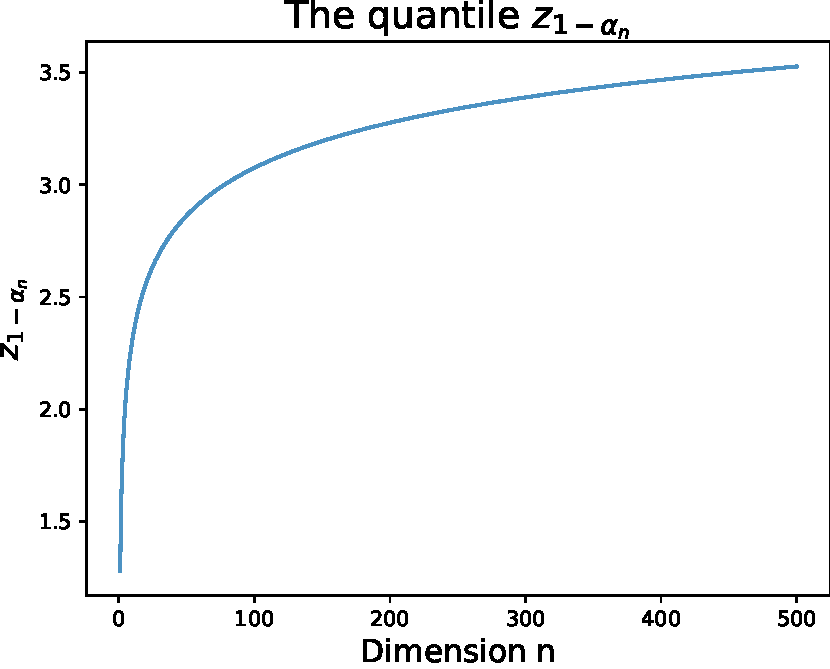
\includegraphics[width=\textwidth]{fig/class_dist_to_winner.pdf}
    \end{minipage}
    \hfill
    \hspace{0.01\textwidth}
    \begin{minipage}{0.33\textwidth}
        \centering
        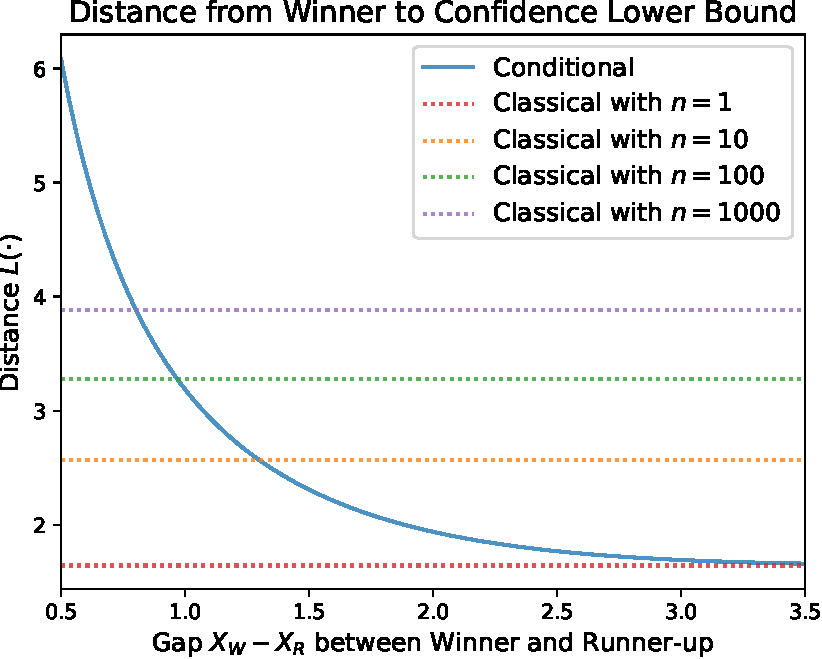
\includegraphics[width=\textwidth]{fig/cond_dist_to_winner.pdf}
    \end{minipage}
    \hfill
    \hspace{0.01\textwidth}
    \begin{minipage}{0.33\textwidth}
        \centering
        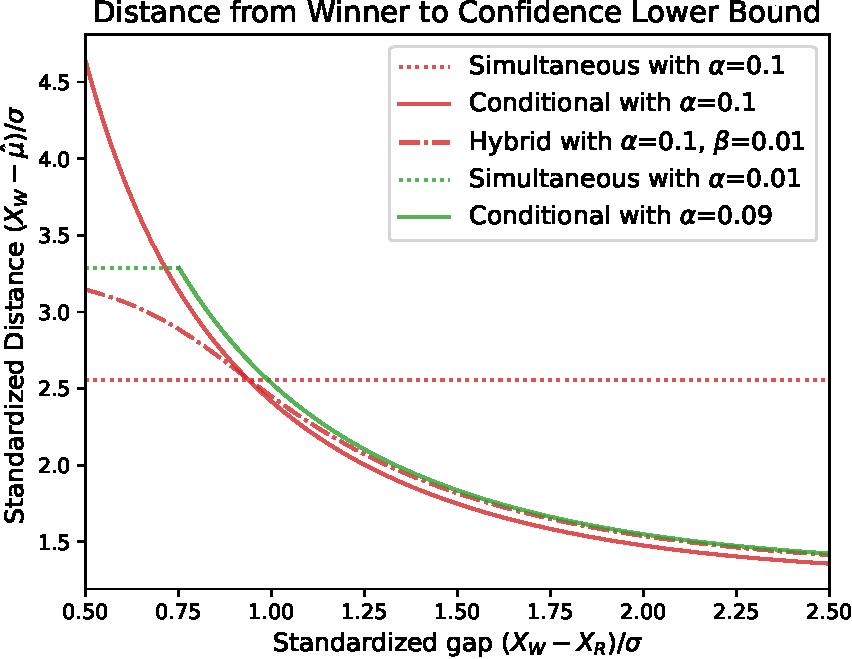
\includegraphics[width=\textwidth]{fig/hyb_dist_to_winner.pdf}
    \end{minipage}
    }
    \caption{ The first panel (left) shows the growth of the quantile $z_{1 - \alpha_n}$ as a function of the dimension $n$. The second panel (middle) gives the distance between the level $\alpha=0.05$ conditional LCB and the winner $X_W$ (i.e., the function $L(\cdot)$ in \eqref{eq:cond_lcb}) as a function of the gap $X_{W} - X_{R}$ between winner and the runner-up. For dimensions $n=1,10,100,1000$, we also give the distance from $X_W$ to the level $\alpha=0.05$ classical LCB. The third panel (right) considers a $n=10$ dimensional problem and shows this distance for the level $\alpha=0.05$ hybrid, conditional, and classical LCBs in red. For hybrid we take $\beta=0.005$. It also shows the distance to the larger of the level $\alpha=0.045$ conditional LCB and level $\alpha=0.005$ classical LCB in green (i.e., the union bound LCB).}
    \label{fig:lcb}
\end{figure}

Again suppose we observe independent Gaussian data $X \sim N(\mu, I_n)$ and want to make a LCB for the mean $\mu_W$ of the winner $W = \argmax_{i \in [n]} X_i$. 

The conditional approach tries to avoid the classical approach's curse of dimensionality by providing inferences for only the winning mean. It does so by delivering an LCB for $\mu_W$ that is valid conditionally on $W$. To construct the conditional LCB, we follow the framework of \cite{Fithian}. Letting $R$ be the index of the runner-up (second largest observation), we note that the deviation of $X_{W}$ from $\mu_{W}$ has a truncated normal distribution once we condition on $W$ and $X_{-W}$:
\begin{equation}
    \label{eq:cond_dist}
    X_W - \mu_W \mid W, X_{-W} \sim TN(0, 1, X_{R} - \mu_{W}, \infty).
\end{equation}
Letting 
\begin{equation}
    \label{eq:cond_quantile}
    q_{1-\alpha}(w, x_{-w}, \mu_w) = \text{Quantile}_{\mu}(1-\alpha, X_W -  \mu_{W} \mid W=w, X_{-w} = x_{-w})
\end{equation}
denote the $1-\alpha$ quantile of this conditional distribution \eqref{eq:cond_dist}, it is straightforward to show that
\begin{equation}
\label{eq:cond_set}
     C_{cond}(X) = \{\eta : \eta > X_{W} - q_{1-\alpha}(W, X_{-W}, \eta)  \} 
\end{equation}
is a $1-\alpha$ confidence region for $\mu_{W}$ that is valid  conditional on $W$ and  $X_{-W}$:
\begin{equation*}
    P_{\mu}( \mu_{W} \in C_{cond}(X) | W, X_{-W})  = P_{\mu}( X_W - \mu_W < q_{1-\alpha}(W, X_{-W}, \mu_{W}) |W, X_W) = 1-\alpha.
\end{equation*}
Since $\eta$ appears on both sides of the membership condition in \eqref{eq:cond_set}, it is not clear that $C_{cond}(X)$ actually provides a lower bound for $\mu_{W}$. We will see, however, that we can rewrite $C_{cond}(X)$ as 
\begin{equation}
\label{eq:cond_lcb}
     C_{cond}(X) = \{\eta : \eta > X_{W} - L(X_W - X_R)  \}. 
\end{equation}
where $L: \R \rightarrow \R$ is a complicated ``length'' function that determines the distance from the winner $X_W$ to the lower confidence bound. We will de-mistify $L(\cdot)$ in the next sub-section. For now, we provide a plot of it in the middle panel of \Cref{fig:lcb}.

As can be seen in \Cref{fig:lcb}, the conditional LCB has very interesting behavior. In some situations, it indeed seems to avoid the curse of dimensionality. If the gap between $X_W$ and $X_R$ is large, then the conditional LCB for $\mu_W$ will be roughly $X_{W} - z_{1-\alpha}$, i.e, what we expect in a one-dimensional inference problem. But the cost of using the conditional approach can be tremendous. As the runner-up gets close to the winner, the conditional LCB goes quickly to $-\infty$ and can give much worse inferences than the classical approach. For example, if the runner-up is within just one standard deviation of the winner, we get inferences similar to those in the $n = 100$ dimensional classical problem. 

Compared to the classical approach, which provides a lower bound that is a fixed distance from the winner, the conditional approach is much harder to interpret. Its quality depends on a somewhat opaque relationship between the runner-up and the winner. How separated does the winner need to be from the runner-up for the conditional approach to be useful? And how close can the winner and runner-up be before the classical approach is better? We shed light on these questions by rewriting the conditional procedure in terms of p-values. 

\subsubsection{The Conditional LCB with p-Values}

As we did for the classical LCB, imagine rejecting the winning null $H^{\mu_0}_{0, W}: \mu_{W} \leq \mu_0$ when the conditional LCB is at least $\mu_0$. Again, we will check this condition by examining the p-values $p^{\mu_0}_i = 1- \Phi(X_i - \mu_0)$. To be more concrete, we will assume $\alpha=0.05$ from now onwards. 

In contrast to the classical LCB, the conditional LCB rejects $H^{\mu_0}_0$ when the winning (smallest) p-value $p^{\mu_0}_{(1)}$ is small relative to the runner-up (second smallest) p-value $p^{\mu_0}_{(2)}$. Particularly, it rejects when $p^{\mu_0}_{(1)} \leq \alpha p^{\mu_0}_{(2)}$. We can therefore write the conditional LCB \eqref{eq:cond_set}, which is composed of all the $\mu_0$ for which we fail to reject $H_{0, W}^{\mu_0}$, as  
\begin{equation}
\label{eq:cond_set_p_val}
    C_{cond}(X) = \{ \mu_0 \in \R:  p^{\mu_0}_{(1)} >  \alpha p^{\mu_0}_{(2)} \}. 
\end{equation}
Derivations verifying these facts can be found in \Cref{sec:cond_appdx}. 


\begin{figure}[]
    \centering
    \scalebox{1}{
    \hspace{-0.03\textwidth}
    \begin{minipage}{0.33\textwidth}
        \centering
        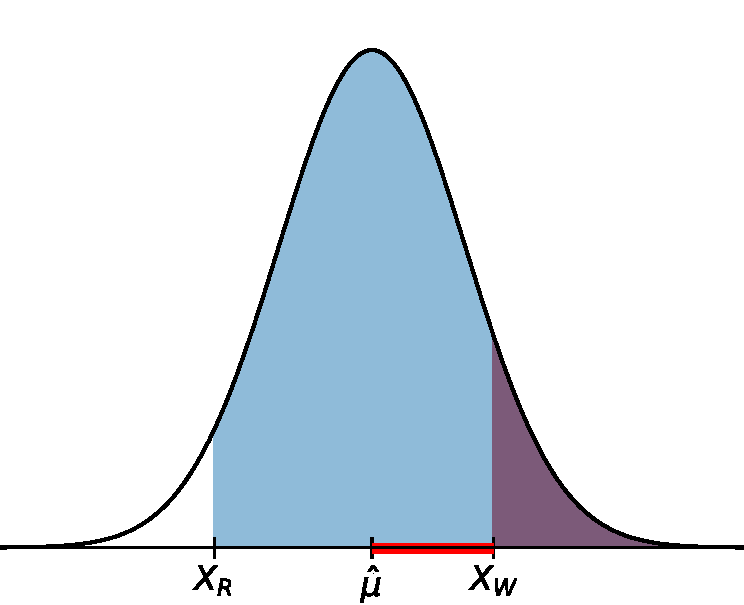
\includegraphics[width=\textwidth]{tail_prob_1.pdf}
    \end{minipage}\hfill
    \hspace{0.02\textwidth}
    \begin{minipage}{0.33\textwidth}
        \centering
        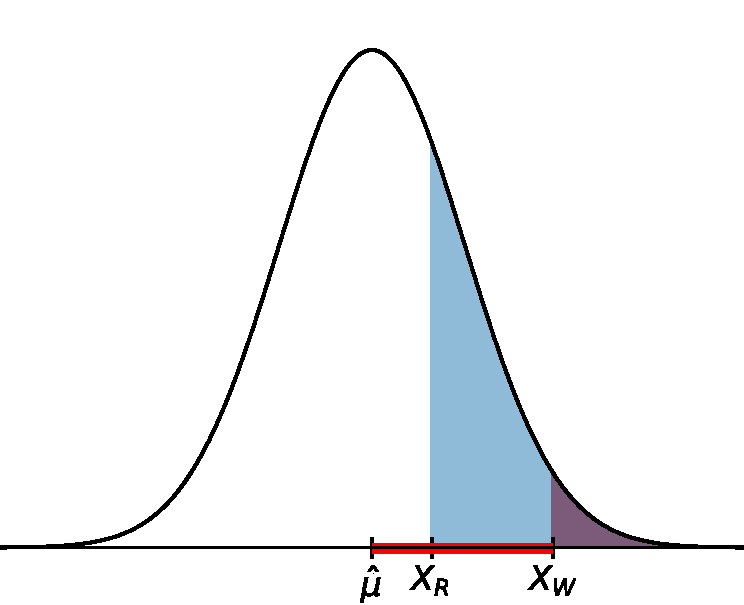
\includegraphics[width=\textwidth]{tail_prob_2.pdf}
    \end{minipage}\hfill
    \hspace{0.02\textwidth}
    \begin{minipage}{0.33\textwidth}
        \centering
        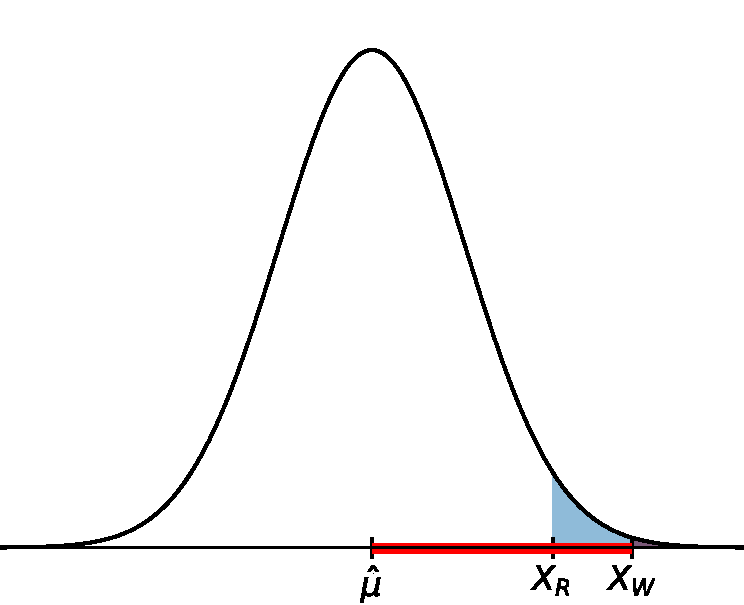
\includegraphics[width=\textwidth]{tail_prob_3.pdf}
    \end{minipage}
    }
    \caption{We plot the level $\alpha=0.1$ conditional LCB $\hat{\mu}$ for different gaps between the winning value $X_W$ and the runner up value $X_R$ and highlight the distance between $\hat{\mu}$ and $X_W$ in red. The LCB $\hat{\mu}$ is chosen exactly so that the tail probability $P(N(\hat{\mu}, 1) > X_R)$, shaded in blue, is $1/\alpha=10$ times the tail probability $P(N(\hat{\mu}, 1) > X_W)$, shaded in red (the overlap appears purple). As $X_W$ and $X_R$ get closer, we need to take $\hat{\mu}$ further and further back for this condition to be satisfied.}
    \label{fig:tail_prob}
\end{figure}

From \eqref{eq:cond_set_p_val} we get a clear interpretation of the length function $L(\cdot)$ from \eqref{eq:cond_lcb}. The conditional LCB stretches all the way back to the mean $\mu_0$ under which it is $1/\alpha = 20$ times less likely to see something as extreme as the winner than something as extreme as the runner-up! It is not hard to show (see \Cref{sec:gap_appdx}) that the distance between $X_W$ and the conditional LCB is determined solely by the gap between $X_W$ and $X_R$. If the winner and runner-up are very close, we will need $\mu_0$ to be very far back. Thanks to the decay of the Gaussian tail, however, we can always find such a mean if we go far back enough. \Cref{fig:tail_prob} provides an illustration. 

As we have already seen in \Cref{exm:winner}, when working with independent and selectively dominant p-values, rejecting the winning null when the smallest p-value is at most $\alpha$ times the second smallest p-value is an error controlling procedure. Equipped with our selective dominance machinery, the computations in \Cref{exm:winner} were quite straightforward. In place of the previous sub-section's computations, it would have been much easier to justify our conditional LCB as an inversion of \Cref{exm:winner}'s test for the winner. For completeness, we restate the result from \Cref{exm:winner} in \Cref{thm:cond}. 

\begin{theorem}[Testing the winner]
    \label{thm:cond}
    Suppose that $p_i$ are $n$ independent and selectively dominant p-values under the nulls $H_{0, i}$, and let $W$ be the index of the smallest p-value. Rejecting $H_{0, W}$ when $p_{(1)} \leq \alpha p_{(2)}$ controls Type I error at level $\alpha$ conditionally on $W$, and therefore also marginally. The same is thus true for rejecting the global null $\cap_{i=1}^n H_{0, i}$ when $p_{(1)} \leq \alpha p_{(2)}$. 
\end{theorem}

Once written in terms of p-values, its easy to see the merits and pitfalls of the conditional approach mathematically. If all the p-values except the smallest provide essentially no evidence against the null (i.e, the winner is well separated), then $p_{(2)} \approx 1$ and we reject when $p_{(1)} < \alpha$, the same p-value cutoff as a one-dimensional problem. On the other hand, if even just one other p-value provides a similar amount of evidence against the null as the smallest p-value, then then $p_{(2)} \approx p_{(1)}$ and we will never reject because $p_{(1)} \not < \alpha p_{(1)} \approx \alpha p_{(2)}$. In general, the conditional approach only makes a discovery if the most extreme observation is $1/\alpha = 20$ more extreme under the null than the second most extreme observation. This can be quite a stringent requirement!  

The p-value viewpoint also makes it clear that the conditional approach can only outperform the classical one when some null p-values are conservative. In our Gaussian problem, the p-value for $H^{\mu_0}_{0, i}: \mu_i \leq \mu_0$ is conservative when $\mu_i \ll \mu_0$. We give a heuristic argument here, and a more formal statement in \Cref{sec:beta_dist_appdx}. Suppose one of our p-values $p_1$ is a very strong signal (i.e., $\mu_1 \gg \mu_0$) but the remaining p-values $p_2, \dots, p_n$ are non-conservative nulls (i.e, $\mu_2, \dots, \mu_n = \mu_0$). Our conditional procedure will reject when our smallest p-value, likely $p_1$, is less than $\alpha$ times the minimum of $p_2, \dots, p_n$, which are $n-1$ independent uniform random variables that have a minimum of $1/n$ on average. Thus, roughly speaking, the conditional approach also rejects when $p_{(1)}$ is less than $\alpha/n \approx \alpha_n$, which is no better than Sidak's. 

Like was the case for our classical procedure, we can make more discoveries via the conditional approach by closing \Cref{thm:cond}'s global null test. Although the resulting procedure is a bit strange, it is interesting that \Cref{thm:cond}'s global null test admits a tractable closure. 

\begin{corollary}[Closed testing for winners]
    \label{cor:cond_closed}
    Suppose that $p_i$ are $n$ independent and selectively dominant p-values under the nulls $H_{0, i}$. As shorthand, let $H_{0, (j)}$ denote the null corresponding to the $j$th smallest p-value and define $p_{(n+1)} = 1$.  Rejecting the null hypotheses $H_{0, (k)}$ for which $p_{(j)} \leq \alpha p_{(j-1)} $ for every $j \leq k$ controls FWER error at level $\alpha$. 
\end{corollary}

This closed procedure is also best understood sequentially. We reject $H_{0, (1)}$ if $p_{(1)} \leq \alpha p_{(2)}$. Then, if we rejected  $H_{0, (1)}$, we reject $H_{0, (2)}$ if $p_{(2)} \leq \alpha p_{(3)}$, so on and so forth until we fail to reject.  

\subsubsection{Generalizing to MLR Families}

Written in terms of p-values, the conditional LCB  \eqref{eq:cond_set_p_val} also easily generalizes to any MLR family. Suppose $P_{\theta}$ is an MLR family and we observe $n$ independent samples $X_i \sim P_{\theta_i}$ where the $\theta_i$ are unknown. Let $p^{\theta_0}_i$ be the UMP p-value for testing $H_{0, i} : \theta_i \leq  \theta_0$ as in \eqref{eq:ump_mlr}.  Because the auxiliary randomness we use in \eqref{eq:ump_mlr} is shared across different $\theta_0$, the index of the smallest p-value will be the same for every $\theta_0$. Hence, we can unambigously define the winning index $W = \argmin_{i \in [n]} p^{\theta_0}_i$ to be the index of the smallest p-value.

\Cref{cor:cond_mlr} tells us how to make an LCB for the winning parameter $\theta_W$ that is valid conditioanlly on $W$. 

\begin{corollary}[Conditional inference for MLR families ]
    \label{cor:cond_mlr}
    Let $P_{\theta}$ be a MLR family parameterized by $\theta \in \R$. If $X_i \sim P_{\theta_i}$ are $n$ independent samples and $p^{\theta_0}_i$ is the UMP p-value \eqref{eq:ump_mlr} for testing $H^{\theta_0}_{0, i} : \theta_i \leq \theta_0 $, then 
    \begin{equation}
    \label{eq:cond_lcb_mlr}
    \{\theta_0 :  p^{\theta_0}_{(1)} > \alpha p^{\theta_0}_{(2)}\} 
    \end{equation}
    is an LCB for $\theta_W$ that holds conditionally on $W$ (and therefore also marginally) with probability exactly $1-\alpha$. 
\end{corollary}

The proof of \Cref{cor:cond_mlr} is essentially that the proposed LCB results from inverting the test of the winning null $H^{\theta_0}_{0, W}: \theta_W \leq \theta_0$ from \Cref{thm:cond}. 

We point out that the distance from the winning value $X_W$ to the conditional LCB \eqref{eq:cond_lcb_mlr} will depend on quickly the tail of $P_{\theta}$ decays. If the the tail decays faster, then the first $\theta_0$ for which the largest observation is $1/\alpha = 20$ times as extreme as the second largest observation will be larger. Seeing as the Gaussian distribution, which has an exponentially decaying tail, still often results in very low lower bounds, we should expect that this distance can often be quite large. 

\subsection{Hybrid Inference}

Lastly we provide the same analysis for hybird inference, which tries to balance the benefits of the classical and conditional approaches. 

\subsubsection{The Hybrid LCB}

Like before, we want to make a LCB for the mean $\mu_{W}$ of the winner $W = \argmax_{i \in [n]} X_i$ in the case of independent Gaussian data $X \sim N(\mu, I_n)$ with unknown mean $\mu \in \R^n$. 

The core idea behind hybrid inference is giving a confidence region $C_{hyb}(X)$ that has a very high probability of containing $\mu_W$ on a ``good'' event $G_{\mu}$. Oddly, this good event depends on the unknown parameter. For some $\beta < \alpha$, we need $G_{\mu}$ to happen with probability at least $1-\beta$. Then, if we ensure that $C_{hyb}(X)$ has at least $(1-\alpha)/(1-\beta)$ coverage on the $G_{\mu}$, it will achieve $1-\alpha$ coverage overall:
\begin{align*}
       P_{\mu}(\mu_{W} \in C_{hyb}(X)) &= P_{\mu}(G_{\mu})P_{\mu}(\mu_{W} \in C_{hyb}(X) | G_{\mu}) + P_{\mu}(G_{\mu}^c)P_{\mu}(\mu_{W} \in C_{hyb}(X) | G_{\mu}^c)\\
       &\geq (1-\beta)\left(\frac{1-\alpha}{1-\beta} \right)\\
       &=1-\alpha.
\end{align*}

Considering some $\beta < \alpha$ and defining $\beta_n = 1 - (1-\beta)^{\frac{1}{n}}$ as in \eqref{eq:bonf_quantile}, our good event is that the confidence lower bounds $X_i -  z_{1-\beta_n}$ for the means $\mu_i$ all simultaneously hold:
\begin{equation*}
    G_{\mu} = \{X_i < \mu_i + z_{1-\beta_n} \text{ for all } i \in [n] \}.
\end{equation*}
From our earlier reasoning, we know that this good event happens with probability exactly $1-\beta$. 

Now, we can make a confidence region that contains the mean with probability at least $(1-\alpha)/(1-\beta)$ on this good event. If we condition on $G_{\mu}$ along with $W$ and $X_{-W}$, the deviation of $X_W$ from $\mu_W$ has a truncated normal distribution like \eqref{eq:cond_dist} that is further truncated from above:
\begin{equation}
    \label{eq:hyb_dist}
    X_W - \mu_W \mid W, X_{-W}, G_{\mu} \sim TN(0, 1, X_{R} - \mu_{W}, z_{1-\beta_n} ).
\end{equation}
On the good event $G_{\mu}$, we always have that $X_R - \mu_{W} < X_W - \mu_{W} < z_{1-\beta_n}$, so the lower truncation is indeed below the upper one. Let
\begin{equation}
\label{eq:hyb_quantile}
    q^{h}_{\frac{1-\alpha}{1-\beta}}(w, x_{-w}, \mu_w) = \text{Quantile}_{\mu}\left(\frac{1-\alpha}{1-\beta}, X_W -  \mu_{W} \mid W=w, X_{-w} = x_{-w}, G_{\mu}\right)
\end{equation}
denote the $(1-\alpha)/(1-\beta)$ quantile of the conditional distribution \eqref{eq:hyb_dist}. Per the prior discussion, the function \eqref{eq:hyb_quantile} only makes sense if the largest value in $x_{-w}$ at most $z_{1-\beta_n}$, and we will take the quantile \eqref{eq:hyb_quantile} to be $-\infty$ if it is not. It is then straightforward to show that
\begin{equation}
\label{eq:hyb_set}
     C_{hyb}(X) = \{\eta : \eta > X_{W} - q^{h}_{\frac{1-\alpha}{1-\beta}}(W, X_{-W}, \eta)  \} 
\end{equation}
contains $\mu_{W}$ with high probability conditional on $W$, $X_{-W}$, and the event $G_{\mu}$:
\begin{equation*}
    P_{\mu}( \mu_{W} \in C_{hyb}(X) | W, X_{-W}, G_{\mu})  = P_{\mu}( X_W - \mu_W < q^{h}_{\frac{1-\alpha}{1-\beta}}(W, X_{-W}, \mu_{W}) |W, X_W, G_{\mu}) = \frac{1-\alpha}{1-\beta}.
\end{equation*}
Based on our earlier discussions, this is sufficient to imply that $C_{hyb}(X)$ from $\eqref{eq:hyb_set}$ will contain $\mu_{W}$ with probability at least $1-\alpha$. 

As was the case for our conditional confidence region \eqref{eq:cond_set}, the hybrid confidence region \eqref{eq:hyb_set} is a little hard to interpret at first. We will get a clearer sense of its benefits when we write it in terms of p-values. As a teaser, the rightmost panel of \Cref{fig:lcb} plots distance between the winner $X_W$ and the hybrid LCB for a $n=10$ dimensional problem. We argue (using our upcoming p-value viewpoint) in \Cref{sec:hybrid_gap_appdx} that, once we fix $\alpha$ and $\beta$, this distance is a function of just the gap $X_W - X_R$ between the winner and runner up and the problem dimension $n$. 

\subsubsection{The Hybrid LCB with p-Values}

As we did for the conditional LCB, imagine rejecting the winning null $H^{\mu_0}_{0, W}: \mu_{W} \leq \mu_0$ when the hybrid LCB is at least $\mu_0$. Again, we will check this condition by examining the p-values $p^{\mu_0}_i = 1- \Phi(X_i - \mu_0)$.  

It turns out that the hybrid LCB allows us to reject $H_{0, W}^{\mu_0}$ when the winning (smallest) p-value is smaller than a mixture of the runner-up (second smallest) p-value and the level $\beta$ classical cutoff:
\begin{equation}
\label{eq:hybrid_cutoff}
    p^{\mu_0}_{(1)}\leq \frac{\alpha-\beta}{1-\beta}p^{\mu_0}_{(2)}  + \left(1 - \frac{\alpha - \beta}{1 - \beta}\right)\beta_n
\end{equation}
Hence, we can write the hybrid LCB \eqref{eq:hyb_set} as 
\begin{equation}
    \label{eq:hyb_set_p_val}
        C_{hyb}(X) = \left\{ \mu_0 \in \R:  p^{\mu_0}_{(1)} > \frac{\alpha-\beta}{1-\beta}p^{\mu_0}_{(2)}  + \left(1 - \frac{\alpha - \beta}{1 - \beta}\right) \beta_n \right\}. 
\end{equation}
The derivations needed to show this can be found in \Cref{sec:hybrid_appdx}. 

\Cref{thm:hyb} tells us that, when our p-values are independent and selectively dominant, rejecting the most promising null according the hybrid cutoff \eqref{eq:hybrid_cutoff} is a Type I error controlling procedure. The derivations required to show this are similar to those in \Cref{exm:winner}, but a bit more involved, so we have moved the proof to the appendix. 

\begin{theorem}[Hybrid test for the winner]
    \label{thm:hyb}
    Suppose that $p_i$ are $n$ independent and selectively dominant p-values under the nulls $H_{0, i}$, let $W$ be the index of the smallest p-value, and fix some $\beta < \alpha$. Rejecting $H_{0, W}$ when 
    \begin{equation}
        \label{eq:hybrid_cutoff_thm}
        p_{(1)} \leq \frac{\alpha-\beta}{1-\beta}p_{(2)}  + \left(1 - \frac{\alpha - \beta}{1 - \beta}\right) \beta_n
    \end{equation} 
    controls Type I error at level $\alpha$. The same is thus true for rejecting the global null $\cap_{i=1}^n H_{0, i}$ whenever \eqref{eq:hybrid_cutoff_thm} holds.   
\end{theorem}

Once written in terms of p-values, it is much easier to see how the hybrid approach balances the benefits of the classical and conditional approaches.  When the other p-values provide essentially no evidence against the null (i.e., $p_{(2)} \approx 1$), hybrid rejects when $p_{(1)}$ is less than a cutoff that is bounded away from zero. Hence, when the winner is well seperated, the hybrid approach avoids the curse of dimensionality, at least on par with the conditional procedure run at level  $(1-\alpha)/(1-\beta)$. On the other hand, even if some other p-value provides as much evidence against the null as the smallest, hybrid still rejects whenever the level $\beta$ classical LCB does. This is because when $p_{(1)} \leq \beta_n$, the hybrid cutoff is a mixture of two things that are larger than $p_{(1)}$, and we will reject. When we set $\beta = 0$ then the hybrid cutoff \eqref{eq:hybrid_cutoff_thm} becomes $\alpha p_{(2)}$ and we recover the conditional method, and if we set $\beta=\alpha$ it becomes $\alpha_n$ and we recover the classical method. 

Interestingly, the hybrid global null test from \Cref{thm:hyb} also admits a tractable closure that allows us to make more discoveries. 

\begin{corollary}[Closed hybrid testing for winners]
    \label{cor:hyb_closed}
    Suppose that $p_i$ are $n$ independent and selectively dominant p-values under the nulls $H_{0, i}$. As shorthand, let $H_{0, (j)}$ denote the null corresponding to the $j$th smallest p-value and define $p_{(n+1)} = 1$. Fixing some $\beta < \alpha$, rejecting the null hypotheses $H_{0, (k)}$ for which
    \begin{equation*}
        p_{(j)} \leq \frac{\alpha - \beta}{1-\beta} p_{(j-1)} + \left(1 - \frac{\alpha - \beta}{1-\beta} \right) \beta_{n - j + 1}   
    \end{equation*}
    for every $j \leq k$ controls FWER error at level $\alpha$. 
\end{corollary}

This closed procedure is also best understood sequentially. We reject $H_{0, (1)}$ if $p_{(1)} \leq \frac{\alpha - \beta}{1-\beta} p_{(2)} + (1 - \frac{\alpha - \beta}{1-\beta}) \beta_n$. Then, if we rejected $H_{0, (1)}$, we reject $H_{0, (2)}$ if $p_{(2)} \leq  \frac{\alpha - \beta}{1-\beta} p_{(3)} + (1 - \frac{\alpha -\beta }{1-\beta}) \beta_{n-1}$, so on and so forth until we fail to reject.  


\subsubsection{Comparison to Union Bound}

In contrast to hybrid inference, a naive union bound approach rejects the winning null whenever the level $\beta$ classical approach rejects or the level $\alpha -\beta$ conditional approach rejects, i.e., it rejects whenever 
\begin{equation}
    \label{eq:union_bound_cutoff}
    p_{(1)} \leq \max\{(\alpha - \beta) p_{(2)}, \beta_n\}.
\end{equation}
The union bound harshly switches between the classical and conditional approaches, whereas the hybrid approach smoothly interpolates between them. This is illustrated in the rightmost panel of \Cref{fig:lcb}, which compares the LCBs resulting from the hybrid versus union bound approaches. 

Written in terms of p-values, we easily see that the hybrid approach dominates the union bound approach. Both methods reject when $p_{(1)} \leq \beta_n$, and when $p_{(1)} > \beta_n$  the hybrid cutoff \eqref{eq:hybrid_cutoff_thm} is clearly strictly larger than the union bound cutoff \eqref{eq:union_bound_cutoff}, meaning hybrid will reject whenever the union bound does and more. There are two reasons hybrid inference out performs the union bound. First, union bounds are not tight and waste some of the Type I error budget. This is captured by the fact that the coefficient on $p_{(2)}$ is larger in the hybrid cutoff \eqref{eq:hybrid_cutoff_thm} than the union bound cutoff \eqref{eq:union_bound_cutoff}.  Second, conditioning on the ``good event'' in the hybrid approach causes an upper truncation in \eqref{eq:hyb_dist}, which results in $\left(1 - \frac{\alpha - \beta}{1 - \beta}\right)\beta_n$ being added to the cutoff \footnote{the authors \cite{Andrews2023} mention these differences between the union bound and hybrid inference in a footnote, but they only point out that hybrid dominates the level $\beta$ classical approach, which is weaker than our statement.}.

Practically speaking, however, hybrid inference typically results in very little improvement over the union bound. This is already somewhat evident in \Cref{fig:lcb}'s rightmost panel, where we see that the hybrid LCB and union bound LCB are very similar. Even when the hybrid cutoff is larger than that of the union bound, it is provably not much larger. We detail why in \Cref{sec:hybrid_sim_appdx}, where we also run a number of simulations comparing the power of the hybrid and union bound approaches. We are hard pressed to find a setting where the hybrid approach results in a meaningful power gain. Hence, we suggest adopting the view that hybrid inference's main contribution is squeezing out the little power that is left from the union bound approach. As it is not computationally more expensive and our p-value viewpoint makes it equally easy to implement, we feel it is still worth using. 


\subsubsection{Generalizing to MLR Families}

Now written in terms of p-values, the hybrid LCB for the winning parameter \eqref{eq:hyb_set_p_val} immediately generalizes to any MLR family. Like before, suppose $P_{\theta}$ is an MLR family and we observe $n$ independent samples $X_i \sim P_{\theta_i}$ where the $\theta_i$ are unknown. Again, let $p^{\theta_0}_i$ be the UMP p-value for testing $H_{0, i} : \theta_i \leq  \theta_0$ as in \eqref{eq:ump_mlr} and let $W = \argmin_{i \in [n]} p^{\theta_0}_i$ be the index of the smallest p-value.

\Cref{cor:hyb_mlr} tells us how to make a hybrid LCB for the winning parameter $\theta_W$. For the same reasons as in the Gaussian setting, the hybrid LCB continues to balance the benefits of the conditional and classical approaches in the more general MLR setting. 

\begin{corollary}[Hybrid inference for MLR families ]
    \label{cor:hyb_mlr}
    Let $P_{\theta}$ be a MLR family parameterized by $\theta \in \R$ and fix some $\beta < \alpha$. If $X_i \sim P_{\theta_i}$ are $n$ independent samples and $p^{\theta_0}_i$ is the UMP p-value \eqref{eq:ump_mlr} for testing $H^{\theta_0}_{0, i} : \theta_i \leq \theta_0 $, then 
    \begin{equation}
            \label{eq:hyb_lcb_mlr}
            \left\{\theta_0 :  p^{\theta_0}_{(1)} \leq \frac{\alpha-\beta}{1-\beta}p^{\theta_0}_{(2)}  + \left(1 - \frac{\alpha - \beta}{1 - \beta}\right) \beta_n \right\}
    \end{equation}
     is an LCB for the winning parameter $\theta_W$ that holds with probability at least $1-\alpha$. 
\end{corollary}

Again, the proof of \Cref{cor:hyb_mlr} is essentially that the proposed LCB is the inversion of the test of the winning null $H^{\theta_0}_{0, W}: \theta_W \leq \theta_0$ from \Cref{thm:hyb}. 


\section{Rank Verification in Exponential Families}
\label{sec:rank_verification}

In this section we consider the problem of verifying that that the winning parameter is actually larger than the other parameters, i.e., rather than doing inference on the winning parameter, we do inference on the gap between the winning parameter and the remaining parameters. Mainly, we give a corrected accounting of the seminal work \cite{Hung2019}'s main results in the language of selected dominance. It illustrates how our selective dominance machinery allows us to correctly design fairly intricate statistical procedures.  

\subsection{Warm-up: Rank Verification and Type III Error Control}

To motivate the rank verification problem and shed some light on how it relates to selective dominance, we consider a seemingly unrelated classical statistical question about Type III errors. 

A friend of yours tests whether the unknown means of two univariate Gaussian samples, $X_1 \sim N(\mu_1, 1/\sqrt{2})$ and $X_2 \sim N(\mu_2, 1/\sqrt{2})$, are different. They end up rejecting the null hypothesis $H_0: \mu_1 = \mu_2$ because the two-sided UMPU p-value $1 - \Phi(|X_1 - X_2|)$ is at most $\alpha$. After rejecting, they note $X_1 > X_2$, and claim ``not only am I confident that the two means are different, but they must be different because $\mu_1$ is bigger than $\mu_2$''. Your friend, however, only rejected the null that the means are equal. Can they make a claim about the direction of inequality? This is a quesiton of Type III error, and we can use our selective dominance framework to show that your friends claims are actually statistically valid. 

Based on their claim, it seems that what your friend really wants to do is test the one-sided null $H_{0, 1} : \mu_1 \leq \mu_2$ whenever they observe that $X_1 > X_2$, and test the complementary one-sided null $H_{0, 2} : \mu_2 \leq \mu_1$ whenever they observe that $X_2 < X_1$. To test the null $H_{0, j} : \mu_{j} \leq \mu_{-j}$ we normally use the UMP p-value  $1 - \Phi(X_j - X_{-j})$. In your friend's case, however, they only select this p-value to use for inference when they observe that $X_j > X_{-j}$, or equivalently that $p_j < 1/2$. \Cref{exm:rank_verification} illustrates how, using our selective dominance framework, your friend could develop a procedure that delivers valid inferences in spite of this selection.  

\begin{example}[Rank verification in a simple case]
\label{exm:rank_verification}
Suppose that $p$ is a selectively dominant p-value for testing the null $H_0$, but we only choose to test $H_0$ when $p < 1/2$. Applying our framework with the p-value $p$ and selection function $s(x) = I_{x < 1/2}$, \Cref{thm:adjustment} tells us that we control selective Type I error if we reject according to the adjusted p-value from \eqref{eq:adjustment} is $p_{adj} = 2p$:
\begin{equation}
    \label{eq:rank_verification_error_control}
    P_{H_{0}}\left(p_j \leq \frac{\alpha}{2} | S = 1\right) \leq \alpha.
\end{equation} 

Now, consider data $X_1 \sim N(\mu_1, 1/\sqrt{2})$ and $X_2 \sim N(\mu_2, 1/\sqrt{2})$, the one-sided nulls $H_{0, j}: \mu_j \leq \mu_{-j}$, and their corresponding selectively dominant p-values $p_j = 1 - \Phi(X_j - X_{-j})$ (selective dominance follows from \Cref{exm:mlr}). Denoting the winner $W = \argmax_{j = 1, 2} X_j$, it is now clear rejecting the data-dependent null $H_{0, W}: \mu_W \leq \mu_{-W}$ when $p_{W} \leq \alpha/2$ maintains Type I error control both conditionally on $W$ and marginally. If $H_{0, j}$ is not true, then trivially $P(\text{falsely reject } H_{0, W} \mid W = j) = 0 \leq \alpha$. For the case that $H_{0, j}$ is true, the event $W=j$ is identical to the event $p_j < 1/2$, and hence is the same event as selecting $p_j$ for inference in \eqref{eq:rank_verification_error_control}. Therefore, 
\begin{align*}
    P(\text{falsely reject } H_{0, W} \mid W = j) &= P\left(p_W \leq \frac{\alpha}{2}  \mid W = j\right)\\
    &= P\left(p_j \leq \frac{\alpha}{2}  \mid W = j \right) \\
    &\leq \alpha,
\end{align*}
implying error control conditional on $W$. Marginal error control then follows from the law of total probability:
\begin{align*}
    P(\text{falsely reject } H_{0, W}) &= \sum_{j=1, 2} P(\text{falsely reject } H_{0, j} \mid W = j)P(W=j) \\
                                      &\leq \alpha \sum_{j = 1, 2} P(W=j)\\
                                      &=\alpha. 
\end{align*}
If $\mu_1 = \mu_2$ then the inequalities become equalities and our error control is tight. 
\end{example}

In \eqref{exm:rank_verification}, we provide a procedure that verifies the rank of the winning mean with Type I error control, i.e., it affirms not just that the means are different, but that the winning mean $\mu_W$ is larger than the other mean.  The procedure, which rejects when the smaller of the two one-sided p-values $p_i = 1 - \Phi(X_i - X_{-i})$ is at most $\alpha/2$, is identical to the procedure that rejects when the two-sided p-value $1 - \Phi(|X_1 - X_2|)$ is at most $\alpha$! Hence, for reasons likely unbeknowst to them, your friend's original claim is indeed statistically valid. 

In what follows, we generalize \eqref{exm:rank_verification}'s rank verification procedure to the exponential family setting. Although this generalization appears quite a bit more complicated, the core idea remains the same. 

\subsection{Rank Verification in Exponential Families}

In this sub-section we illustrate how to do rank verification when we observe data $X \in \R^m$ from a multiparameter exponential family $P_{\theta}$ with density
\begin{equation}
    \label{eq:exp_fam}
    g_{\theta}(x) = \exp(\theta_1 T_1(x) + \dots + \theta_n T_n(x) - \psi(\theta))g(x)
\end{equation}
We typically care about doing inference on some subset $\mathcal{S} \subseteq [p]$ of the $\theta_j$ (e.g., in the case of a multivariate Gaussian with unknown covariance $\sigma^2I_n$, we usually are only interested in $\theta_j$ that determine the means and not the $\theta_j$ that determines the variance). Since $E_{\theta}[T] = \theta$, it makes sense to let the winner $W$ be the index in $\mathcal{S}$ corresponding to the largest sufficient statistic $T_i$, with ties broken randomly.

Considering the nulls $H^{\delta}_{0, ij} : \theta_i - \theta_j \leq \delta $, we want to reject the data-dependent global null $\cap_{j \in \mathcal{S} - W} H^{\delta}_{0, Wj} $ and affirm that $\theta_W$ is more than $\delta$ larger than any other parameter in $\mathcal{S}$. Then we can make an LCB for the difference $\theta_W - \max_{j \in \mathcal{S} - W } \theta_j$ between the winning and next largest parameter in $\mathcal{S}$ by inverting this test. 

Considering some $i\neq j$, we start by constructing the UMPU p-value $p^{\delta}_{ij}(X)$ for testing $H_{0, ij}^{\delta}: \theta_i - \theta_j \leq \delta$. Defining the transformed sufficient statistics $\widetilde{T} \in \R^n$ by
\begin{equation}
    \label{eq:reparam}
    \widetilde{T}_i = \frac{T_i - T_j}{2}, \qquad  \widetilde{T}_j = \frac{T_i + T_j}{2}, \qquad  \widetilde{T}_{\ell} = T_{\ell} \text{ for } \ell \neq i, j
\end{equation}
we can reparametrize the density \eqref{eq:exp_fam} as 
\begin{equation}
    \label{eq:exp_fam}
    g_{\theta}(x) = \exp\left( (\theta_i - \theta_j) \widetilde{T}_i + (\theta_i + \theta_j) \widetilde{T}_j + \sum_{\ell \neq i, j} \widetilde{T}_{\ell} \theta_{\ell} \right)g(x).
\end{equation}
From this reparameterization, it is clear that the conditional left-continuous survival function of $\widetilde{T}_i$ and its righthand limit 
\begin{equation}
    G^{\delta}_{ij}(\tilde{t}_i | \tilde{t}_{-i}) = P_{\theta_i - \theta_j = \delta}(\widetilde{T}_i \geq \tilde{t}_i | \widetilde{T}_{-i} = \tilde{t}_{-i}) \qquad G_{ij}^{\delta, +}(\tilde{t}_i | \tilde{t}_{-i}) = \lim_{u \downarrow \tilde{t}_i } G^{\delta}_{ij}(u | \tilde{t}_{-i}),
\end{equation}
have no dependence on $\theta$, and the UMPU p-value $p^{\delta}_{ij}$ for testing $H_{0, ij}^{\delta}: \theta_i - \theta_j \leq \delta$ is given by 
\begin{equation}
    \label{eq:umpu_rank_verification}
    p_{ij}^{\delta}(X) = G^{\delta, +}_{ij}(\widetilde{T}_i | \widetilde{T}_{-i}) + U_{ij, aux}(G^{\theta_0}_{ij}(\widetilde{T}_{i}|\widetilde{T}_{-i}) - G^{\theta_0, +}_{ij}(\widetilde{T}_i|\widetilde{T}_{-i})),
\end{equation}
where $U_{ij, aux}$ are $\text{Unif}([0,1])$ random variables that are independent from each other and $X$ (see Chapter Four of \cite{Lehmann} and \Cref{sec:mlr_selective_dominance_appdx} for a justification).

Crucially, we can tell if $i \in \mathcal{S}$ is a winner by examining $p^{\delta}_{ij}$. It is straightforward to confirm that $i \in \mathcal{S}$ is the sole winner exactly when $\widetilde{T}_i > \max_{k \in \mathcal{S} - i} \widetilde{T}_k - \widetilde{T}_j $. Equivalently, this happens when $p^{\delta}_{ij}$ is strictly smaller than 
\begin{equation}
    \label{eq:rank_verification_lower}
    q^{\delta, +}_{ij}(\widetilde{T}_{-i}) = G^{\delta, +}_{ij}(\max_{k \in \mathcal{S} - i} \widetilde{T}_k - \widetilde{T}_j | \widetilde{T}_{-i}).
\end{equation}
Likewise, one can confirm that $i \in \mathcal{S}$ is one of multiple winners in $\mathcal{S}$ exactly when $\widetilde{T}_i = \max_{k \in \mathcal{S} - i} \widetilde{T}_k - \widetilde{T}_j$, or equivalently when $p^{\delta}_{ij}$ is at least $q^{\delta, +}_{ij}$ but at most 
\begin{equation}
    \label{eq:rank_verification_upper}
    q^{\delta}_{ij}(\widetilde{T}_{-i}) = G^{\delta}_{ij}(\max_{k \in \mathcal{S} - i} \widetilde{T}_k - \widetilde{T}_j | \widetilde{T}_{-i}),
\end{equation}
Moreover, in the case that there are multiple winners, the number of winners is also a deterministic function of $\widetilde{T}_{-i}$:
\begin{equation}
    \label{eq:rank_verification_num_ties}
    N_{i}(\widetilde{T}_{-i}) = 1 + \{ k \in \mathcal{S} - i : \widetilde{T}_k = \max_{\ell \in \mathcal{S} - i} \widetilde{T}_{\ell} \}.
\end{equation}
Note that $N_{i}(\widetilde{T}_{-i})$, which is always at least two, is \underline{not} the same as the number of winners, which can be one. Rather, it is the number of winners there will be if $\widetilde{T}_i$ is a winner and at least one other $\widetilde{T}_j$ is as well.  

Leveraging these facts, \Cref{exm:rank_verification_exp_fam} shows how we can use our selective dominance framework to come up with valid tests for both the winning null $H^{\delta}_{Wj}$ and the winning global null  $\cap_{j \in \mathcal{S} - W} H^{\delta}_{0, Wj}$. 

\begin{example}
    \label{exm:rank_verification_exp_fam}
    Suppose $p$ is a p-value for the null $H_0$ that is selectively dominant given $Z$. If we select $p$ to use for inference according to the selection function 
    \begin{equation*}
        s(x, z) = 
        \begin{cases} 
        1 & \text{if } x < q^+(z), \\
        \frac{1}{N(z)} & \text{if } x \in [q^+(z), q(z)], \\
        0 & \text{otherwise},
        \end{cases},
    \end{equation*}
    where $N(z)> 1$ and $0 \leq q^{+}(z) \leq q(z) \leq 1$ are known functions of $z$, then the adjusted p-value from \eqref{eq:adjustment} turns out to be (see \Cref{sec:rank_verficiation_adj_appdx} for computations)
    \begin{equation}
            \label{eq:tie_adj_p_val}
            p_{adj} = f(p, q^+(Z), q(Z), N(Z)) \qquad f(a, b, c, d) =   \frac{a - (1 - \frac{1}{d})(a - b)_+}{b + \frac{1}{d}(c - b)}. 
     \end{equation}
    Therefore, \Cref{thm:adjustment} tells us that rejecting when \eqref{eq:tie_adj_p_val} is at most $\alpha$ is a selective Type I error controlling procedure:
    \begin{equation}
        \label{eq:tie_tool}
        P_{H_0}\left(f(p, q^+(Z), q(Z), N(Z))  \leq \alpha \mid Z, S = 1\right) \leq \alpha.  
    \end{equation} 

    Now, suppose we observe $X$ drawn from the exponential family \eqref{eq:exp_fam} and let $W$ be the index $i \in \mathcal{S}$ of the largest sufficient satistic (with ties broken randomly). For $i \neq j$, \Cref{exm:exp_fam} tells us that the UMPU p-value $p = p_{ij}^{\delta}$ from \eqref{eq:umpu_rank_verification} for the null $H_{0, ij}^{\delta}: \theta_i - \theta_j \leq \delta$ is selectively dominant given the transformed nuisance statistics $Z = \widetilde{T}_{-i}$ from \eqref{eq:reparam}. Taking $q^+(Z) = q^{\delta, +}_{ij}( \widetilde{T}_{-i})$, $q(Z) = q^{\delta}_{ij}( \widetilde{T}_{-i})$, $N(Z) = N_{i}(\widetilde{T}_{-i})$ and $f$ from  \eqref{eq:rank_verification_lower}, \eqref{eq:rank_verification_upper}, \eqref{eq:rank_verification_num_ties}, and \eqref{eq:tie_adj_p_val}, it is now easy to show that rejecting the data-dependent null $H^{\delta}_{0, Wj}$ when $f(p^{\delta}_{Wj}, q^{\delta, +}_{Wj}, q^{\delta}_{Wj}, N_{W}) \leq \alpha$ controls Type I error both conditional on $W$ and marginally. Again it suffices to restrict our attention to indices $i \in \mathcal{I}$, $i \neq j$ that have a positive probability of being the winner (if $i=j$, then we know $H^0_{ii}$ is true and we simply do not reject). If $H^{\delta}_{0, ij}$ is not true, then trivially $P(\text{falsely reject } H^{\delta}_{0, Wj}| W= i) = 0 \leq \alpha$. For the case that $H^{\delta}_{0, Wj}$ is true (and $i \neq j$), the event $W=i$ is the same event as selecting $p_{0, ij}^{\delta}$ for inference in \eqref{eq:tie_adj_p_val}, so 
    \begin{align*}
        P(\text{falsely reject } H^{\delta}_{0, Wj}| W= i) &= P(f(p^{\delta}_{Wj}, q^{\delta, +}_{Wj}, q^{\delta}_{Wj}, N_{Wj}) \leq \alpha | W= i) \\
        &= P(f(p^{\delta}_{ij}, q^{\delta, +}_{ij}, q^{\delta}_{ij}, N_i) \leq \alpha | W = i) \\
        &\leq \alpha. 
    \end{align*}
    Marginal error control follows from the usual law of total probability argument.

    We can reject the data-dependent global null when  $\cap_{j \in \mathcal{S} - W} H^{\delta}_{0, Wj}$ when we reject all of the individual nulls $H^{\delta}_{0, Wj}$ for $j \in \mathcal{S} - W$. It is straightforward to see that this will control Type I error both conditionally on $W$ and marginally: If there is an $i \in \mathcal{I}$ for which $\cap_{j \in \mathcal{S} - i} H^{\delta}_{0, ij}$ is false, then trivially $P(\text{falsely reject } \cap_{j \in \mathcal{S} - W} H^{\delta}_{0, Wj}| W= i) = 0 \leq \alpha$ for this $i$. Otherwise, there exists a $k \in \mathcal{S} - i$ for which $\theta_i \leq \theta_k$, and 
    \begin{align*}
        P(\text{falsely reject } \cap_{j \in \mathcal{S} - W} H^{\delta}_{0, Wj}| W= i) \leq P(\text{falsely reject } H^{\delta}_{0, Wk}| W= i) \leq \alpha.\
    \end{align*} 
    Again, marginal error control follows from the usual law of total probability argument.
\end{example}

By inverting \Cref{exm:rank_verification_exp_fam}'s test for the data-dependent global null $\cap_{j \in \mathcal{S} - W} H^{\delta}_{0, Wj}$, we can get our desired LCB for $\theta_W - \max_{j \in \mathcal{S} - W } \theta_j$. We give a precise statement in \Cref{thm:rank_verification} below. 

\begin{theorem}
    \label{thm:rank_verification}
    Let $X$ be drawn from the exponential family \eqref{eq:exp_fam} and let $W$ be the index $i \in \mathcal{S}$ corresponding to the largest sufficient statistic $T_i$ (with ties broken randomly). If $p^{\delta}_{ij}$ is the UMPU p-value \eqref{eq:umpu_rank_verification} for testing $H^{\delta}_{0, ij} : \theta_i - \theta_j \leq \delta$ and $q^{\delta, +}_{ij}$, $q^{\delta}_{ij}$, and $N_{i}$ are as in \eqref{eq:rank_verification_lower},  \eqref{eq:rank_verification_upper}, and \eqref{eq:exp_fam_num_ties}, then 
    \begin{equation}
    \label{eq:rank_verification_lcb}
    \left\{\delta : \max_{j \in \mathcal{S} - W} \frac{p^{\delta}_{Wj} - \left(1 - \frac{1}{N_{i}} \right)(p^{\delta}_{Wj} - q^{\delta, +}_{Wj})_+ }{q^{\delta, +}_{Wj} + \frac{1}{N_{i}}(q^{\delta}_{Wj} - q^{\delta, +}_{Wj}) } > \alpha \right\} 
    \end{equation}
    is a LCB for $\theta_W$ that holds with probability at least $1 - \alpha$
    conditionally on $W$ (and therefore also marginally). 
\end{theorem}

\begin{figure}[]
    \centering
    \scalebox{1}{
    \begin{minipage}{0.49\textwidth}
        \centering
        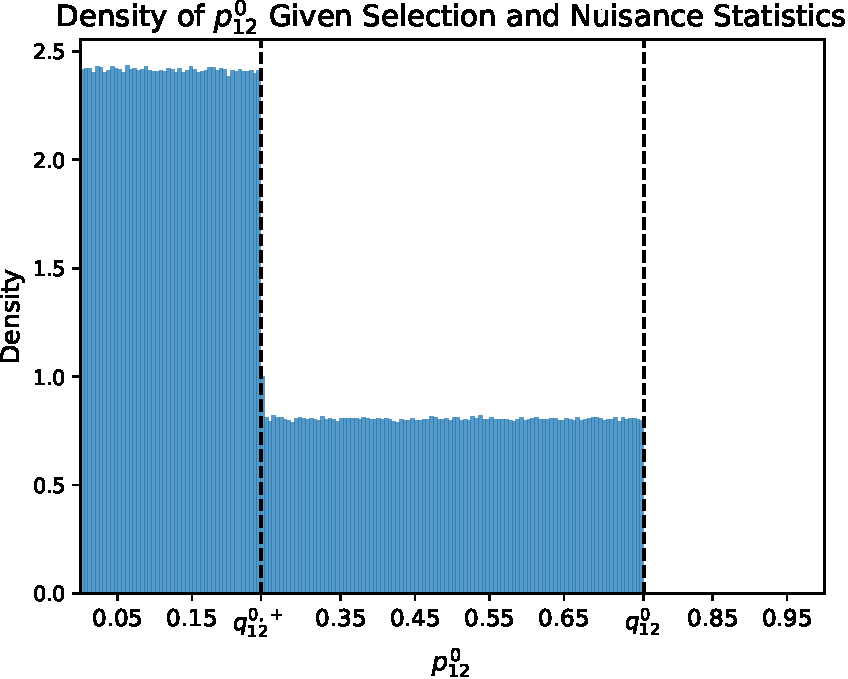
\includegraphics[width=\textwidth]{p_val_density.pdf}
    \end{minipage}\hfill
    \raisebox{0.18cm}{
    \begin{minipage}{0.49\textwidth}
        \centering
        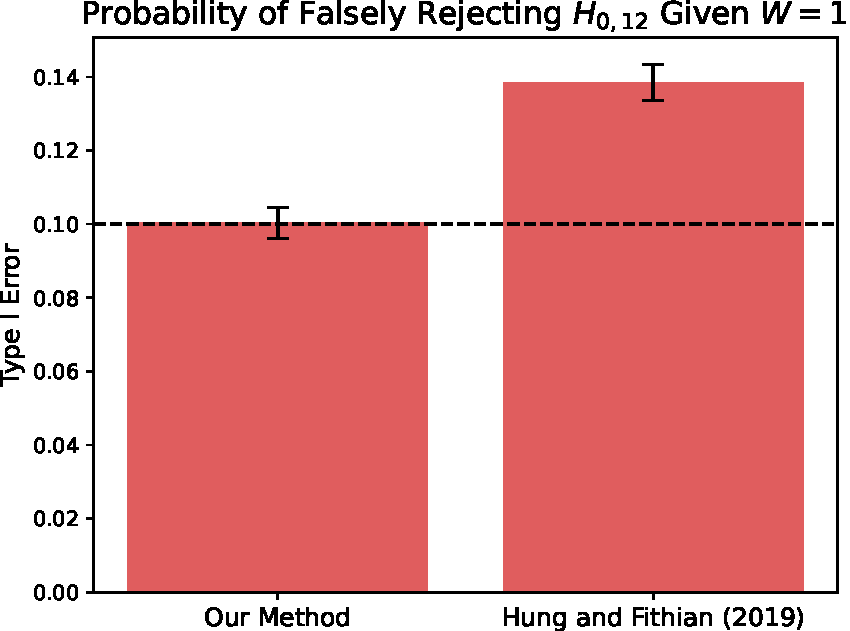
\includegraphics[width=\textwidth]{type_one_error.pdf}
    \end{minipage}\hfill
    }}
    \caption{Considering three independent binomial random variables $X_i \sim \text{Bin}(n, s_i)$ with random variables with $n=4$ and $s_i = 1/2$, the first panel (left) depicts $N=10^6$ draws from the conditional distribution of the p-value $p^{0}_{12}$ (used for testing $H^{0}_{0, 12}: s_1 \leq s_2$) given selection $W= 1$ and the nuisance statistics $(X_1 + X_2)/2 = 4$, $X=3$. When $p_{12}^0  < q^{0, +}_{12}$, then $X_1$ is the sole winner and the p-value is selected for inference with probability one, but when $p_{12}^0 \in [q^{0, +}_{12}, q^0_{12}]$ there is a three-way tie and it is selected for inference with probability $1/3$. Hence, the p-value's conditional distribution is not uniform on $[0, q^0_{12}]$ as \cite{Hung2019} implicitly assume. The next panel (right) displays the consequence. Conditional on $W=1$, \cite{Hung2019} do not maintain Type I error control when testing $H^{0}_{W2}$ at level $\alpha=0.1$ (denoted by horizontal dashed line), whereas our method does. Error bars denote a 99\% confidence interval.}
    \label{fig:error_control}
\end{figure}

Our derivation of the test for $H_{0, Wj}$ differs from that given in \cite{Hung2019} in two important ways. First, the derivation in \cite{Hung2019} only implies Type I error control at the boundary of the one-sided null, although they assume it to be true for the entire composite null. Due to selection, establishing validity for entire composite null is non-trivial. Thankfully, it is immediately implied by our selective dominance machinery and \Cref{exm:exp_fam}. Second, \cite{Hung2019} incorrectly use the same adjusted p-value when there are and are not ties amongst the $T_j$. If there cannot be ties amongst the $T_j$, then $q^{\delta}_{ij} = q^{\delta, +}_{ij}$ and the adjusted p-value \eqref{eq:tie_adj_p_val} we use to test $H^{\delta}_{0, ij}$ conditional on $W = i$ simplifies to $p^{\delta}_{ij}/q^{\delta}_{ij}$. If we use $p^{\delta}_{ij}/q^{\delta}_{ij}$ as our adjusted p-value when ties are possible, we will not achieve conditional error control (as is claimed in \cite{Fithian}). In the case that $X \in \R^3$ is three independent binomials, the left panel of \Cref{fig:error_control} depicts the conditional distribution of $p^{0}_{12}$ given $W=1$ and a specific setting of the nusiances statistics $Z$. It makes it clear that rejecting when $p^{\delta}_{ij}/q^{\delta}_{ij} < \alpha $ does not maintain error control, as affirmed in \Cref{fig:error_control}'s right panel. 

In closing, we mention that the the final result (\Cref{thm:rank_verification}) is perhaps not as surprising as \cite{Hung2019} originally suggest. In \cite{Hung2019}, there are further computations showing that if the exponential family density \eqref{eq:exp_fam} is such that $T(X) = X$, the function $g(x)$ is Schur concave (see \cite[Definition 2]{Fithian}), and there are no ties, then (1) the maximum in \eqref{eq:rank_verification_lcb} is achieved by the runner up $R$ (the index $j \in S$ with second largest sufficient statistic $T_j$) and (2) $q^{0}_{WR}$ is equal to $1/2$. Hence, in this restricted setting, we can claim that the winning parameter is indeed the largest whenever $p^{0}_{WR} \leq \alpha/2$, i.e., whenever the two-sided test comparing the winner and runner-up rejects. Since this test has non-vanishing level even as $n$ grows, the authors claim that it seems to surprisingly circumvent a multiple comparisons issue. However, \Cref{exm:rank_verification} already illustrates why verifying rank by running a two-sided test comparing the winner and loser gives Type I error control in the $n=2$ dimensional case. It should be obvious then that running a two-sided test to compare the winner to the best of $n-1$ losers in the $n > 2$ dimensional case is a more conservative procedure. In other words, the multiplicty correction does not appear in the level of the test, but it is baked in by the fact that we compare the winner to the largest of $n-1$ different losers, which scales with $n$. 

\subsection{Inference on Winners in Exponential Families}

We can use the same tools from the previous sub-section  to do inference on the winner in multiparameter exponential families. Again consider data $X$ drawn from the exponential family \eqref{eq:exp_fam} and let the winner $W$ be the index $i \in \mathcal{S} \subseteq [p]$ corresponding to the largest sufficient statistic $T_i$, with ties broken randomly.

The p-value 
\begin{equation}
    \label{eq:ump_exp_fam}
    p_i^{\theta_0}(T(X)) = G^{\theta_0, +}_i(T_i|T_{-i}) + U_{i, aux}(G^{\theta_0}_i(T_i|T_{-i}) - G^{\theta_0, +}_i(T_i|T_{-i})),
\end{equation}
corresponds to the UMP test for $H_{0, i}^{\theta_0}: \theta_i \leq \theta_0$, where, like before,
\begin{equation*}
    G^{\theta_0}_i(t_i | t_{-i}) = P_{\theta_0}(T_i \geq t | T_{-i} = t_{-i}) \qquad G^{\theta_0, +}_i(t) = \lim_{u \downarrow t}(T_i \geq t | T_{-i} = t_{-i} ),
\end{equation*}
denote the conditional left-continuous survival function of $T_i$ and its right-hand limit, and $U_{i, aux}$ are $\text{Unif}([0,1])$ random variables that are independent from each other and $X$.

To come up with a test for the data dependent null $H_{0, W}^{\theta_0}$ (which we will then invert to get an LCB for the winning parameter), we need to apply a similar adjustment to our p-value as in \Cref{exm:rank_verification_exp_fam}. Rather than re-work through essentially identical arguments, we simply define the analogous quantities to those from the previous sub-section,
\begin{equation}
    \label{eq:exp_fam_lower}
    q^{\theta_0, +}_i(T_{-i}) = G^{\theta_0, +}_i(\max_{k \in \mathcal{S} - i } T_k | T_{-i}), 
\end{equation} 
\begin{equation}
    \label{eq:exp_fam_upper}
    q^{\theta_0}_i(T_{-i}) = G^{\theta_0}_i(\max_{k \in \mathcal{S} - i } T_k | T_{-i}),
\end{equation} 
\begin{equation}
    \label{eq:exp_fam_num_ties}
    N_i(T_{-i}) = 1 + | \{k \neq i: T_k = \max_{\ell \in \mathcal{S} - i} T_\ell \}|,
\end{equation}
and state the final result in \Cref{cor:cond_exp_fam}. In \Cref{coming_soon} we use a modification of the arguments in \cite{Fithian} to show that our test $H^{\theta_0}_{0, W}$ is selectively UMPU, meaning it is UMPU amongst all tests that are are valid conditional on $W$. Hence, as stated in \Cref{cor:cond_exp_fam}, its inversion is selectively uniformly most accurate unbaised (UMAU) in the analogous sense. 

\begin{corollary}[Conditional inference for multiparameter exponential families ]
    \label{cor:cond_exp_fam}
    Let $X$ be drawn from the exponential family \eqref{eq:exp_fam} and let $W$ be the index $i \in \mathcal{S}$ corresponding to the largest sufficient statistic $T_i$ (with ties broken randomly). If $p^{\theta_0}_i$ is the UMP p-value \eqref{eq:ump_exp_fam} for testing $H^{\theta_0}_{0, i} : \theta_i \leq \theta_0 $ and $q^{\theta_0, +}_i$, $q^{\theta_0}_i$, and $N_i$ are as in \eqref{eq:exp_fam_lower}, \eqref{eq:exp_fam_upper}, and \eqref{eq:exp_fam_num_ties}, then 
    \begin{equation}
    \label{eq:cond_lcb_exp_fam}
    \left\{\theta_0 :  \frac{p^{\theta_0}_W - \left(1 - \frac{1}{N_i} \right)(p^{\theta_0}_W - q^{\theta_0, +}_W)_+ }{q^{\theta_0, +}_W + \frac{1}{N_i}(q^{\theta_0}_W - q^{\theta_0, +}_W) } > \alpha \right\} 
    \end{equation}
    is an LCB for $\theta_W$ that holds with probability exactly $1-\alpha$ conditional on $W$ (and therefore also marginally), and it is selectively UMAU conditional on $W$.
\end{corollary}

Briefly, we point out that selecting the largest sufficient statistic does not always correspond to selecting the ``most promising'' effect. Even though $T_i > T_j$, it might be the case that $p^{\theta_0}_{j}$ is smaller than $p^{\theta_0}_{i}$.  Unlike in \Cref{sec:winner}, we cannot simply have the winner correspond to the smallest p-value for two reasons. First, in this more general setting, the index resulting in the smallest p-value changes depending on $\theta_0$ (see \Cref{sec:small_p_val_appdx} for an example). Hence, it is not well-defined to determine the winner by looking at the smallest p-value (and we thus have to deal with ties). Second, even if we settled on a $\theta_0$ to prioritize, because the p-values have intricate correlation strucutre, the selection event $p^{\theta_0}_{i} < \max_{j \neq i} p^{\theta_0}_{j}$ corresponds to a very complicated selection function that we would have to try and characterize on a case-by-case basis. Indeed, this discussion applies to the rank verification problem for exponential families we discussed previously as well. 

\section{New Selective Methods}

In this section we illustrate how our selective dominance framework allows us to easily design new methods for selective inference, global null testing, and dealing with publication bias.   

Rather than just selecting just one p-value as in \Cref{sec:dominance}, some of this section's methods select multiple p-values to use for inference. As such, we need to slightly generalize our framework from \Cref{sec:dominance}. The generalization is intuitive, and for sake of brevity we have deferred a formal account of it to \Cref{sec:multiple_p_vals_appdx}. The proofs of validity for this section's methods, which are in the appendix, often rely on \Cref{sec:multiple_p_vals_appdx}. 

\subsection{Simultaneous Inference on the Top $k$}

Rather than doing inference on just the most promising effect, we may want to do simultaneous inference on the top $k$ most promising effects. Written in terms of p-values, it is easy to give a conditional inferential procedure that does just that. 
\begin{corollary}[Testing the top $k$ winners]
    \label{cor:cond_top_k}
    Suppose that $p_i$ are $n$ independent and selectively dominant p-values under the nulls $H_{0, i}$ and let $H_{0, (j)}$ denote the null corresponding to the $j$th smallest p-value. Rejecting all $H_{0, (j)}$ for which $p_{(j)} \leq \alpha_k p_{(k+1)}$ controlls FWER at level $\alpha$ condititional on the indices of the smallest $k$ p-values (and therefore also marginally). 
\end{corollary}
If the $k+1$ smallest p-value provides close to no evidence against the null (i.e., $p_{(k)} \approx 1$), then \Cref{cor:cond_top_k} corresponds to applying Sidak's procedure to the smallest $k$ p-values, totally ignoring that there were $n$ p-values to start. On the other hand, if $p_{(j)}$ not $1/\alpha_k$ times smaller than $p_{(k+ 1)}$, \Cref{cor:cond_top_k} will fail to reject $H_{0, (j)}$. In the parametric setting of \Cref{sec:class_mlr}, we get simultaneously valid conditional LCBs for the top $k$ winning parameters (parameters corresponding to the $k$ smallest p-values) by inverting \Cref{cor:cond_top_k}'s tests. 


Similarly, it is straightforward to do simultaneous hybrid infernce on the top $k$ parameters. 
\begin{corollary}[Hybrid testing the top $k$ winners]
    \label{cor:hyb_top_k}
    Suppose that $p_i$ are $n$ independent and selectively dominant p-values under the nulls $H_{0, i}$. As shorthand, let $H_{0, (j)}$ denote the null corresponding to the $j$th smallest p-value. Fixing some $\beta < \alpha_k$, rejecting all $H_{0, (j)}$ for which 
    \begin{equation}
        p_{(j)} \leq  \frac{\alpha_k - \beta}{1-\beta}p_{(k + 1)} + \left( 1 - \frac{\alpha_k - \beta}{1-\beta} \right) \beta_n
    \end{equation}
    controlls FWER at level $\alpha$.
\end{corollary}

Like before, simultaneous hybrid inference maintains some benefits of conditional simultaneous inference while never doing worse than level $\beta$ classical inference (where now $\beta$ is at most $\alpha_k$). Again, in \Cref{sec:class_mlr}'s parameteric setting, we can get simultaneously valid hybrid LCBs for the top $k$ winning parameters by inverting \Cref{cor:hyb_top_k}'s tests. 

\subsection{Adaptive Versions of Fisher's Combination Test}

\begin{figure}
    \centering
    \hspace{-0.035\textwidth}
    \begin{minipage}{0.32\textwidth}
        \centering
        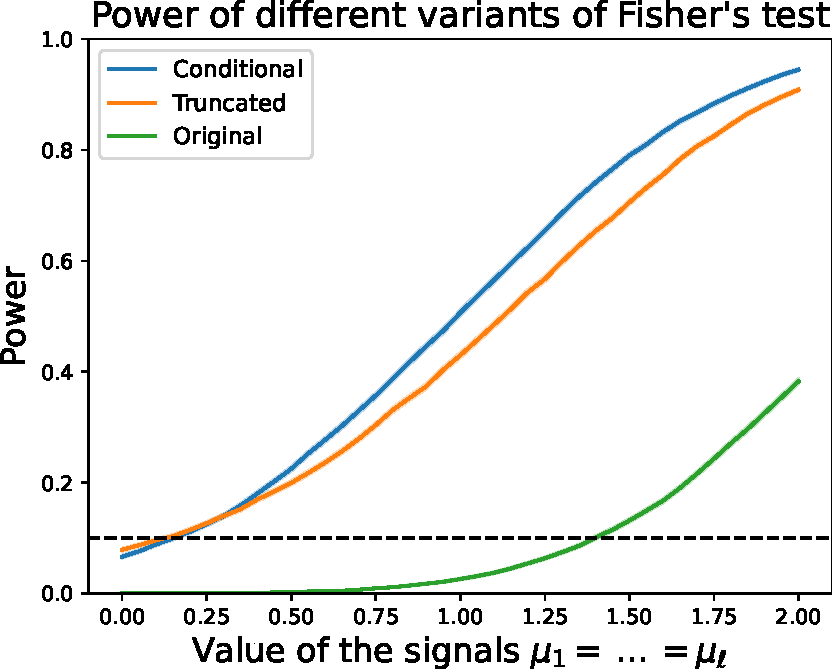
\includegraphics[width=\textwidth]{fig/fisher_ell=3.pdf}
        \caption*{(a) $\ell=3$}
    \end{minipage}
    \hfill
    \hspace{0.01\textwidth}
    \begin{minipage}{0.32\textwidth}
        \centering
        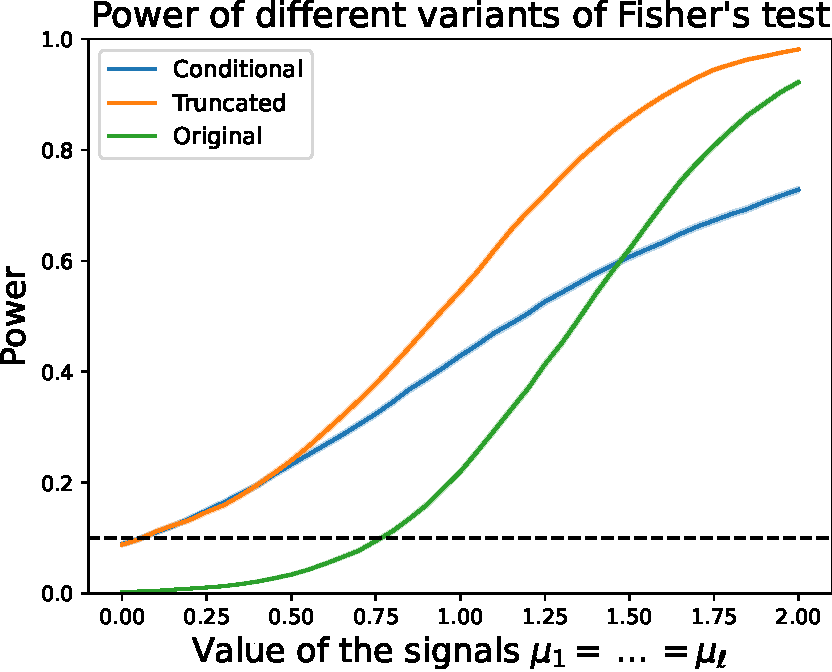
\includegraphics[width=\textwidth]{fig/fisher_ell=5.pdf}
        \caption*{(b) $\ell=5$}
    \end{minipage}
    \hfill
    \hspace{0.01\textwidth}
    \begin{minipage}{0.32\textwidth}
        \centering
        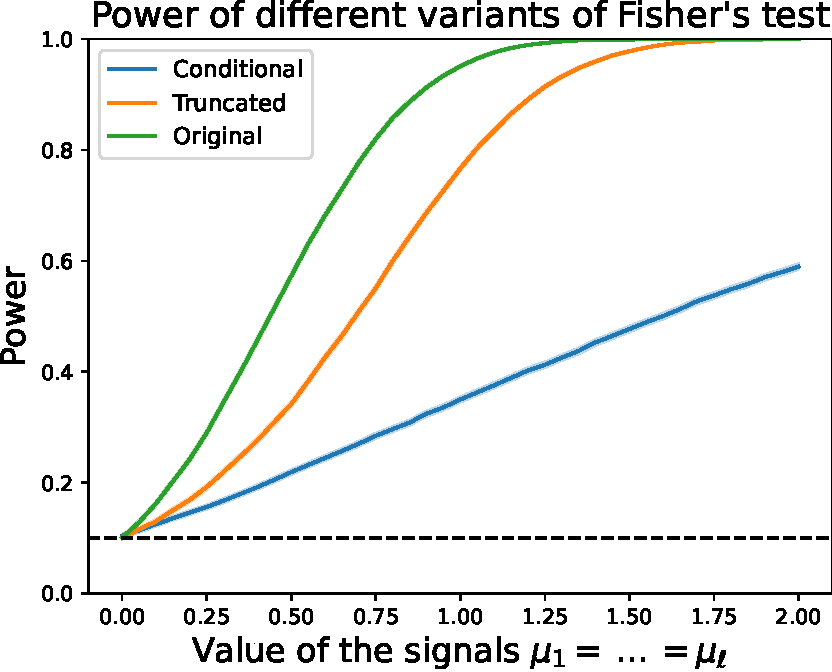
\includegraphics[width=\textwidth]{fig/fisher_ell=10.pdf}
        \caption*{(c) $\ell=10$}
    \end{minipage}
    \caption{ For $\ell=3$ (left), $\ell=5$ (middle), and $\ell=10$ (right), power of the top $k=3$ conditional, $\tau=0.5$ truncated, and original Fisher's combination test for data drawn from $N(\mu, I_{10})$ with $\mu_{1}= \dots = \mu_{\ell}$ varying according to the x-axis and $\mu_{\ell + 1} = \dots = \mu_n = -2$. Power results from an average over $N=10^4$ trials, bands denote one standard error (barely visible), and the level $\alpha=0.1$ is denoted by the dashed line.}
    \label{fig:fisher}
\end{figure}

If we are just interested in verifying the existence of a signal, we can try and combine inferences on the top $k$ effects rather than trying to simultaneous inference on them individually. This is made possible by \Cref{cor:cfisher}, which gives a conditional version of Fisher's combination test. Recall that Fisher's original combination test considers $n$ independent p-values $p_i$ for the nulls $H_{0, i}$ and rejects the global null $\cap_{i=1}^n H_{i, 0}$ when the test statistic $-2 \sum_{i=1}^n \log(p_i) $ is at least as large as the $1-\alpha$ quantile of the $\chi^2_{2n}$ distribution. 

\begin{corollary}
    \label{cor:cfisher}
    Suppose that $p_i$ are $n$ independent and selectively dominant p-values under the nulls $H_{0, i}$ and let $H_{0, (j)}$ denote the null corresponding to the $j$th smallest p-value. Rejecting the data-dependent global null $\cap_{j=1}^k H_{0, (j)}$ (and therefore also the global null $\cap_{i=1}^n H_{0, i}$) when 
    \begin{equation}
        \label{eq:fisher_conditional}
        -2 \sum_{j=1}^k \log(p_{(j)}/p_{(k+1)}) \geq \text{Quantile}(1-\alpha, \chi^2_{2k})
    \end{equation}
    controls Type I error at level $\alpha$ conditional on the indicies of the smallest $k$ p-values (and therefore also marginally). 
\end{corollary}

Examining \eqref{eq:fisher_conditional}, we see that when the $(k+1)$st p-value provides essentially no evidence against the null (so $p_{(k+1)} \approx 1$), running \Cref{cor:cfisher}'s test is like running Fisher's test using just the top $k$ p-values, completely ignoring that we selected from $n$ of them. In this case, our test statistic will have an essentially identical value to Fisher's original test statistic, but the critical value required for rejection will be much smaller. On the flipside, if many of the $p_{(j)}$ for $j \leq k$ are not sufficiently smaller than $p_{(k+1)}$, then \Cref{cor:cfisher}'s test statistic will be small and the test will fail to reject.

Another approach to improving Fisher's combination test is truncation: only add a p-value to Fisher's statistic if it is below some fixed threshold $\tau \in \R$ \citep{Zaykin}. Past and previous work, however, only establishes validity of this test when the null p-values have exact $\text{Unif[0, 1]}$ distributions, excluding the possbility of one-sided null hypotheses \citep{Zhang}.  \Cref{cor:tfisher}, however, gives a generalized version of Fisher's truncated combination test that is still valid whenever the p-values are independent and selectively dominant.

\begin{corollary}
    \label{cor:tfisher}
    Suppose that $p_i$ are $n$ independent and selectively dominant p-values under the nulls $H_{0, i}$ and fix $n$ thresholds $\tau_i \in [0, 1]$. Letting $j \in J$ denote the random set of indices for which $p_j \leq \tau_j$, rejecting the data-dependent global null $\cap_{j \in J} H_{0, j}$ (and therefore also the global null $\cap_{i=1}^n H_{0, i}$) when 
    \begin{equation*}
        -2 \sum_{j=1}^k \log(p_j/\tau_j) \geq \text{Quantile}(1-\alpha, \chi^2_{2|J|})
    \end{equation*} 
    controls type I error at level $\alpha$ conditional on which indicies are in $J$ (and therefore also marginally). 
\end{corollary}

If some $p_j$ are substantially lower than their truncation point $\tau_j$ but most are above it, compared to Fisher's original combination test, \Cref{cor:tfisher}'s test will use a slightly smaller test statistic but a much smaller critical value. Hence, the truncated Fisher test is most powerful when some p-values come from strong alternatives but many p-values come from conservative nulls. (i.e, the null p-values do not have exact $\text{Unif}([0, 1])$ distributions). As such, \Cref{cor:tfisher} actually generalizes the truncated Fisher test to the settings where it is most useful. On the flipside, if most of the $p_j$ are below $\tau_j$, the truncated test statistic pays a penalty due to selection while, compared to Fisher's original test, the test's critical value remains essentially unchanged. 

To illustrate the benefits and drawbacks of these methods, we display their power alongside that of Fisher's original test for a simple $n=10$ dimensional Gaussian problem, where we sample $X \sim N(\mu, I_n)$ and use the p-values $p_i = 1 - \Phi(X_i)$ try and detect the existence of a positive mean. For $\ell \in \{3, 5, 10\}$, we vary the strength $\mu_1 = \dots = \mu_{\ell} > 0$ of our signals and set $\mu_{\ell + 1} = \dots = \mu_n = -2$ to be conservative nulls. We do inference on the top $k=3$ p-values using the conditional version of Fisher's method and set the truncation $\tau = 0.5$ for the truncated version (i.e., we include $p_i$ for which $X_i > 0$). The results are displayed in \Cref{fig:fisher}

As expected, the new methods outperform Fisher's original method when conservative nulls are present. When $\ell=3$ and the bottom three p-values are much smaller than the rest, the conditional method does incredibly well. But its performance quickly degrades when $\ell = 5, 10$ and the fourth smallest p-value becomes often close to the bottom three. By focusing inference on just the top five p-values, the truncated method still considerably improves power when $\ell=5$. Unsurprisingly, both methods perform worse than Fisher's original method when $\ell=10$ and every $\mu_i$ is a signal. 


\subsection{Selecting by the Biggest Gap}

As we saw previously, methods for doing inference using the top $k$ effects can be powerful, but they are plagued by the question of how to choose $k$. These methods work well when the ratio between $p_{(k)}$ and $p_{(k+1)}$ is large, but poorly otherwise. This begs the question, why not select the p-value $p_{(j)}$ whose ratio with $p_{(j+1)}$ is the largest?

\begin{theorem}
    \label{thm:ratio_testing}
    Suppose that $p_i$ are $n$ independent and selectively dominant p-values under the nulls $H_{0, i}$. Defining $p_{(0)}=0$ and $p_{(n+1)}=1$, let $G_j = \frac{p_{(j)} - p_{(j - 1)}}{p_{(j+1)} - p_{(j)}}$ be the gap... Defining $W = \argmax_{j \in [p]} G_j$ as the index of the largest gap, the procedure that rejects $H_{0, W}$ when 
    \begin{equation}
        \label{eq:gap_cutoff}
        p_{(W)} \leq \alpha (G_{(2)}\alpha p_{(W+1) + (1 - G_{(2)}p_{(W - 1)}) })   
    \end{equation}
    controls Type I error at level $\alpha$ conditional on $W$ (and therefore also marginally)
\end{theorem}

 

\subsection{Correcting for Publication Bias}

Selectively dominant p-values also allow us to make valid inferences in the presence of publication bias. Under two models of publication bias, we use our selective dominance machinery to argue that the reader can be confident that a study's result is significant when the associated p-value is at most $\alpha^2$, even if they are worried about publication bias. \newline 

\noindent \textbf{Filtered Studies: } Suppose that a study tests the null $H_0$ at significance level $\alpha$ using a selectively dominant p-value $p$. If the study is only written-up and accepted for publication when the test is significant, then the study is essentially selecting $p$ to use for inference when $p \leq \alpha$ (i.e., the selection function is $s(x) = I_{x \leq 1/2}$). \Cref{thm:adjustment} tells us that, to account for this selection, we should reject when the adjusted p-value $p/\alpha$ is at most $\alpha$. In other words, we still control (selective) Type I error if we reject when $p \leq \alpha^2$. More generally, we show in \Cref{sec:publication_bias_appdx} that rejecting when $p \leq \alpha^2$ controls selective Type I error whenever the authors or publishers are using a selection function that is constant on $[0, \alpha]$ and potentially non-zero on $(\alpha, 1]$ (some non-significant p-values may be published). \newline 

\noindent \textbf{p-Hacking: } Rather than discard a study after observing a p-value that is more than $\alpha$, a researcher may continue making tweaks to their analysis until the p-value crosses the significance threshold. This process, known as p-hacking, encompasses a vast range of techniques, and has therefore been noted to be difficult to study theoretically \citep{Hung2020}. It has been emprically well established, however, that p-hacked p-values have a left-skewed distribution under the null, i.e. p-hacked p-values can be reasonably modeled as having an increasing density under the null with support on $[0,\alpha]$ \citep{Simonsohn, Hung2020}. The transformed p-value $p/\alpha$ then has an increasing density on $[0, 1]$ under the null, and \Cref{thm:density} therefore tells us that $p/\alpha$ is a (selectively dominant) p-value. Thus we can still control Type I error if we reject when $p/\alpha \leq \alpha \iff p \leq \alpha^2$. \newline  

If, in the presence of publication bias, we want to combine evidence from independent studies using selectively dominant p-values, we can run Fisher's truncated combination test (\Cref{cor:tfisher}) with truncation point $\tau_j = \alpha$ for studies we think suffer from publication bias and $\tau_j = 1$ for those that we think do not (e.g., we may not suspect publication bias if a study reports a p-value larger than $\alpha$, or if we are running a new study and are only concerned about publication bias in the previous studies). This combination test, however, requires very strong signals to reject, and, like the procedure of rejecting when $p < \alpha^2$, it will be very conservative if publication bias is not actually present. 

\section*{Acknowledgements}
We thank John Cherian, Yash Nair, and Will Hartog for helpful discussions.

\bibliographystyle{plainnat}
\bibliography{bibliography.bib}

\begin{appendix}

\section{Additional Derivations, Details, and Comments}

\subsection{Distance Between $X_W$ and Conditional LCB }
\label{sec:gap_appdx}

Consider observing Gaussian data $X \sim N(\mu, I_n)$ and let $W$ and $R$ be the indicies of the winner and runner up respectively. We briefly justify that the distance between $X_W$ and the conditional LCB for $\mu_W$ depends only on the gap between $X_W - X_R$. Define $D = X_W - \mu_0$ to be distance between $X_W$ and the conditional LCB $\hat{\mu}$. The conditional LCB $\hat{\mu}$ satisfies 
\begin{equation*}
    \frac{p^{\hat{\mu}}(X_W)}{p^{\hat{\mu}}(X_R)} = \alpha \iff \frac{1 - \Phi(X_W - \hat{\mu})}{1 - \Phi(X_R - \hat{\mu})} = \alpha \iff \frac{1 - \Phi(D)}{1 - \Phi(D - (X_W - X_R))} =\alpha.
\end{equation*}
Clearly then $D$ is a function of $X_W - X_R$.


\subsection{Comparing Conditional and Sidak Global Null Testing}
\label{sec:beta_dist_appdx}

We consider a setting where we have $n$ independent and selectively dominant p-values $p_1, \dots, p_n$ that are all anti-conservative, i.e.,  $p_j \preceq \text{Unif}([0, 1])$. At worst, these p-values are exact uniforms (e.g., they come from the boundary of the null). 

We will show that, on an event with probability at least $1-\epsilon$, the conditional procedure, which rejects when $p_{(1)} \leq \alpha p_{(2)}$, can only reject if $p_{(1)} \leq C_{\epsilon}/n$ for some constant $C_{\epsilon} > 0$. Hence, without conservative nulls, the conditional approach behaves roughly on the same order as the classical approach (Sidak).   

Letting $U_1, \dots, U_n$ be independent $\text{Unif}([0, 1])$ random variables, two facts are clear. First that $U_{(2)} \sim \text{Beta}(2, n-1)$ has mean $\frac{2}{n + 1} < \frac{2}{n}$ and standard deviation $\sqrt{\frac{2(n-1)}{(n+1)^2(n+2)}} \leq \frac{2}{n}$, and second that $p_{(2)} \preceq U_{(2)}$. 

Fix any $\epsilon > 0$. We have by Chebyshev's inequality that  
\begin{align*}
    P\left(p_{(2)} \leq \frac{2}{n}(1 + \epsilon^{-\frac{1}{2}})\right) &\geq P(p_{(2)} \leq E[U_{(2)}] + \sqrt{\Var(U_{(2)})}/\sqrt{\epsilon})\\
    &\geq P(U_{(2)} \leq E[U_{(2)}] + \sqrt{\Var(U_{(2)})}/\sqrt{\epsilon})\\
    &\geq P(|U_{(2)} - E[U_{(2)}]| < \sqrt{\Var(U_{(2)})}/\sqrt{\epsilon} ) \\
    &\geq 1 - \epsilon
\end{align*}
Define $C_{\epsilon} = 2(1 + \epsilon^{-\frac{1}{2}})\alpha$ and the event $A_{\epsilon} = \{ p_{(2)} \leq \frac{2}{n}(1 + \epsilon^{-\frac{1}{2}})\}$. The event $A_{\epsilon}$ has probability at least $1-\epsilon$, and on this event a the conditional procedure never rejects when the procedure $p_{(1)} > C_{\epsilon}/n$, completing our claim. 

In other words, the conditional procedure can only reject when $p_{(1)} \leq C_{\epsilon}/n$ (except for a small probability event) and hence suffers the same curse of dimensionality as the classical method:
\begin{equation*}
    P(p_{(1)} \leq \alpha p_{2} \text{ and } p_{(1)} > C_{\epsilon}/n) \leq P(A_{\epsilon}^c) \leq \epsilon.  
\end{equation*}

\subsection{Distance Between $X_W$ and Hybrid LCB }
\label{sec:hybrid_gap_appdx}

Consider observing Gaussian data $X \sim N(\mu, I_n)$ and let $W$ and $R$ be the indicies of the winner and runner up respectively. We briefly justify that the distance between $X_W$ and the chybrid LCB for $\mu_W$ depends only on the gap between $X_W - X_R$ and the dimension $n$. Define $D = X_W - \mu_0$ to be distance between $X_W$ and the hybrid LCB $\hat{\mu}$. The hybrid LCB $\hat{\mu}$ satisfies 
\begin{align*}
    & p^{\hat{\mu}}(X_W) = \frac{\alpha-\beta}{1-\beta} p^{\hat{\mu}}(X_R) + \left(1 - \frac{\alpha-\beta}{1-\beta} \right)\beta_n\\
    & 1 - \Phi(X_W - \hat{\mu}) = \frac{\alpha-\beta}{1-\beta} (1 - \Phi(X_R - \hat{\mu})) + \left(1 - \frac{\alpha-\beta}{1-\beta} \right)\beta_n\\ 
    &\iff 1 - \Phi(D) = \frac{\alpha-\beta}{1-\beta} (1 - \Phi(D - (X_W - X_R))) + \left(1 - \frac{\alpha-\beta}{1-\beta} \right)\beta_n.
\end{align*}
Clearly then $D$ is a function of $X_W - X_R$ and $n$.

%\subsection{More on Conditional Confidence Regions for the Winner}
%\label{sec:conditional_confidence_region_appdx}

%In \ref{sec:..} we show that the set
%\begin{equation*}
%    \{ \mu_0 \in \R:  (1- \frac{\alpha}{2})p_{(2), \mu_0} > p_{(1), \mu_0} >  \frac{\alpha}{2} p_{(2), \mu_0} \}
%\end{equation*}
%corresponds to the standard two-sided conditional confidence interval (CI) for the mean $\mu_W$ of the winner, and we also discuss how to construct such conditional CIs and CLBs in non-Gaussian settings.  


%\subsection{The p-Value Viewpoint and CLB for the Winner under Correlation}
%\label{sec:conditional_correlation_appdx}

%When working with Gaussian data, we can still do inference on winners in the presence of correlations. In the independent case, we could write the event $W = i $ of $X_i$ winning as $X_i$ being larger than $\max_{j \neq i} X_j$, a random variable that is independent of $X_i$. This independence is what allows us to establish that the conditional distribution \eqref{eq:cond_dist} we used for inference is a truncated normal. In the dependent case where $X \sim N(\mu, \Sigma)$ has unknown mean $\mu$ but known covariance $\Sigma$, we can do the same thing. Because the observations have difference variance, it makes most sense for the winner $W = \argmax_{i \in [p]} X_i/\sqrt{\Sigma_{ii}} $ to correspond to the largest entry after standardization 

%Defining the residual vector $\epsilon_{i}(X) \in \R^n$ with entries $\epsilon_{ij}(X) = X_j - \frac{\Sigma_{ji}}{\Sigma_{ii}}$, it turns out that that (1) $X_i$ and $\epsilon_{ij}(X)$ are independent (2) we can write the winning event as 
%\begin{equation*}
%    \{ W = i \} \iff \{ \}
%\end{equation*}

%The key insight is to write the winning event $W = i$

%If the data is Gaussian, the same trick allows us to do inference on winners with p-values. Defining  $q_i = 1 - \Phi(\max_{j \neq i} \epsilon_{ij}(X) ) $

%The same trick allows us to do inference on winners. Now the selection event $S_i = i$ of selecting the $i$th p-value because it was the lowest amounts to truncating $p_i$ to be smaller than 
\subsection{The p-Value Viewpoint of Conditional Inference}
\label{sec:cond_appdx}

Considering data $X \sim N(\mu, I_n)$ with unknown mean $\mu$ and the p-values $p^{\mu_0
}_i = 1 - \Phi(X_i - \mu_0)$, we want to characterize when the conditional LCB is at least $\mu_0 \in \R$. This happens exactly when $\mu_0$ is not included in the set \eqref{eq:cond_set}. Examining \eqref{eq:cond_dist}, \eqref{eq:cond_quantile}, and \eqref{eq:cond_set}, this happens when $X_W - \mu_0$ is at least as large as the $1-\alpha$ quantile $Q$ of a standard normal truncated to be larger than $X_R - \mu_0$. This quantile satisfies 
    \begin{equation*}
        \alpha = \frac{1 - \Phi(Q) }{1 - \Phi(X_R - \mu_0) }.
    \end{equation*}
Solving for $Q$ gives $Q = \Phi^{-1}(1 - \alpha(1 - \Phi(X_R - \mu_0)))$, meaning we reject exactly when 
\begin{align*}
    X_{W} - \mu_0 \geq \Phi^{-1}(1 - \alpha(1 - \Phi(X_{R} - \mu_0))) &\iff 1 - \Phi(X_{W} - \mu_0) \leq \alpha(1 - \Phi(X_{R} - \mu_0))\\
    &\iff p^{\mu_0}_{(1)} \leq \alpha p^{\mu_0}_{(2)}.
\end{align*}


\subsection{The p-Value Viewpoint of Hybrid Inference}
\label{sec:hybrid_appdx}

Considering data $X \sim N(\mu, I_n)$ with unknown mean $\mu$ and the p-values $p^{\mu_0
}_i = 1 - \Phi(X_i - \mu_0)$, we want to characterize when the hybrid LCB is at least $\mu_0 \in \R$. Examining \eqref{eq:hyb_dist}, \eqref{eq:hyb_quantile}, and \eqref{eq:hyb_set}, we can consider two cases to figure out when this happens. \newline 


\noindent \textbf{Case One - $X_R - \mu_0 \geq z_{1 - \beta_n}$:} If $X_R - \mu_0 \geq z_{1 - \beta_n}$, then $q^h_{\frac{1-\alpha}{1-\beta}}(W, X_{-W}, \mu_0) = -\infty$, so $\mu_0$ cannot be in \eqref{eq:hyb_set}. This case happens precisely when 
\begin{equation*}
    X_R-\mu_0 \geq z_{1 - \beta_n} \iff 1 - \Phi(X_R - \mu_0) \leq 1 - \Phi(z_{1- \beta_n}) \iff p^{\mu_0}_{(2)} \leq \beta_n.
\end{equation*}

\noindent \textbf{Case Two - $X_R - \mu_0 < z_{1 - \beta_n}$:} If $X_R - \mu_0 < z_{1 - \beta_n}$, then $\mu_0$ is not in \eqref{eq:hyb_set} exactly when $X_W - \mu_0$ is at least as large as the $\frac{1-\alpha}{1-\beta}$ quantile $Q$ of a standard normal truncated to be larger than $X_{R} - \mu_0$ but smaller than $z_{1- \beta_n}$. This quantile satisfies 
\begin{equation*}
    \frac{\alpha - \beta}{1- \beta} = \frac{\Phi(z_{1 - \beta_n})  - \Phi(Q) }{\Phi(z_{1-\beta_n})  - \Phi(X_R - \mu_0) } = \frac{1 - \beta_n  - \Phi(Q) }{1 - \beta_n - \Phi(X_R - \mu_0) } 
\end{equation*}
Solving for $Q$ gives 
\begin{equation*}
    Q = \Phi^{-1} \left(1 - \beta_n - \frac{\alpha - \beta}{1 - \beta}\left(1 - \beta_n - \Phi(X_{R} - \mu_0) \right) \right) = \Phi^{-1} \left( \left(1 - \frac{\alpha - \beta}{1 - \beta}\right) (1 - \beta_n) + \frac{\alpha-\beta}{1-\beta}\Phi(X_{R} - \mu_0) \right),
\end{equation*}
so we reject exactly when 
\begin{align*}
        X_{W} - \mu_0 \geq \Phi^{-1} \left( \left(1 - \frac{\alpha - \beta}{1 - \beta}\right) (1- \beta_n) + \frac{\alpha-\beta}{1-\beta}\Phi(X_{R} - \mu_0) \right) \\
        \iff 1 -\Phi(X_{W} - \mu_0) \leq \left(1 - \frac{\alpha - \beta}{1 - \beta}\right)\beta_n + \frac{\alpha-\beta}{1-\beta}(1-\Phi(X_{R} - \mu_0))  \\
        \iff p^{\mu_0}_{(1)} \leq \frac{\alpha-\beta}{1-\beta}p^{\mu_0}_{(2)}  + \left(1 - \frac{\alpha - \beta}{1 - \beta}\right)\beta_n \\
\end{align*}

It turns out we can combine these two cases. Because $p^{\mu_0}_{(1)} \leq p^{\mu_0}_{(2)}$, the fact that $p^{\mu_0}_{(2)} \leq  \beta_n$ in Case One implies that $p^{\mu_0}_{(1)} \leq \beta_n$ also. Therefore in Case One, $p^{\mu_0}_{(1)}$ must be strictly smaller than a mixture of $p^{\mu_0}_{(2)}$ and $\beta_n$:
\begin{equation}
    \label{eq:hybrid_cuttoff_appdx}
    p^{\mu_0}_{(1)} \leq  \frac{\alpha-\beta}{1-\beta}p^{\mu_0}_{(2)}  + \left(1 - \frac{\alpha - \beta}{1 - \beta}\right)\beta_n. 
\end{equation}
Therefore, if we reject according to \eqref{eq:hybrid_cuttoff_appdx}, we will always reject in Case One, and we will reject at the appropriate times in Case Two. 

\subsection{Comparing Hybrid Inference to the Union Bound}
\label{sec:hybrid_sim_appdx}

\begin{figure}
    \centering
    \hspace{-0.035\textwidth}
    \begin{minipage}{0.32\textwidth}
        \centering
        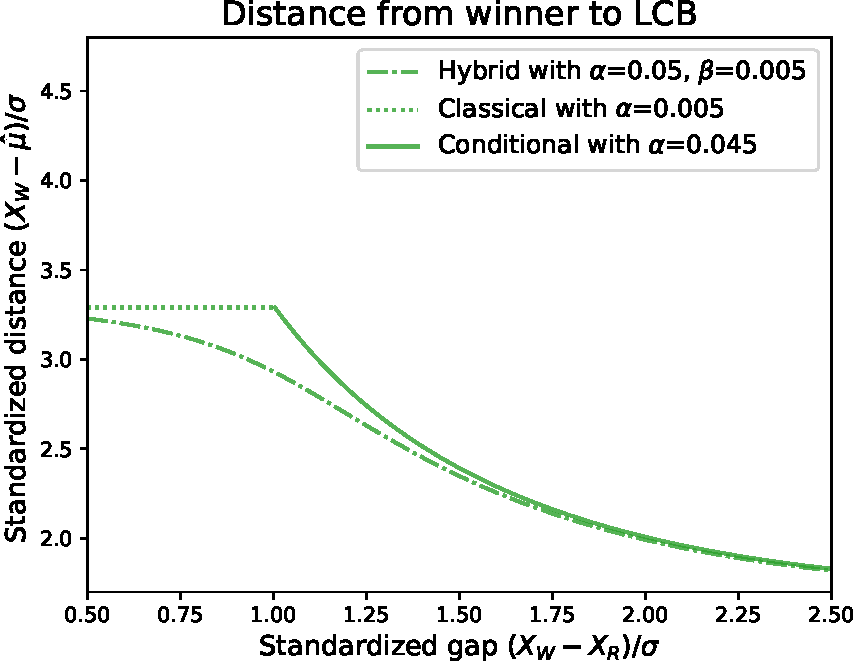
\includegraphics[width=\textwidth]{fig/hyb_dist_to_winner_n=10.pdf}
        \caption*{(a) $n=10$}
    \end{minipage}
    \hfill
    \hspace{0.01\textwidth}
    \begin{minipage}{0.32\textwidth}
        \centering
        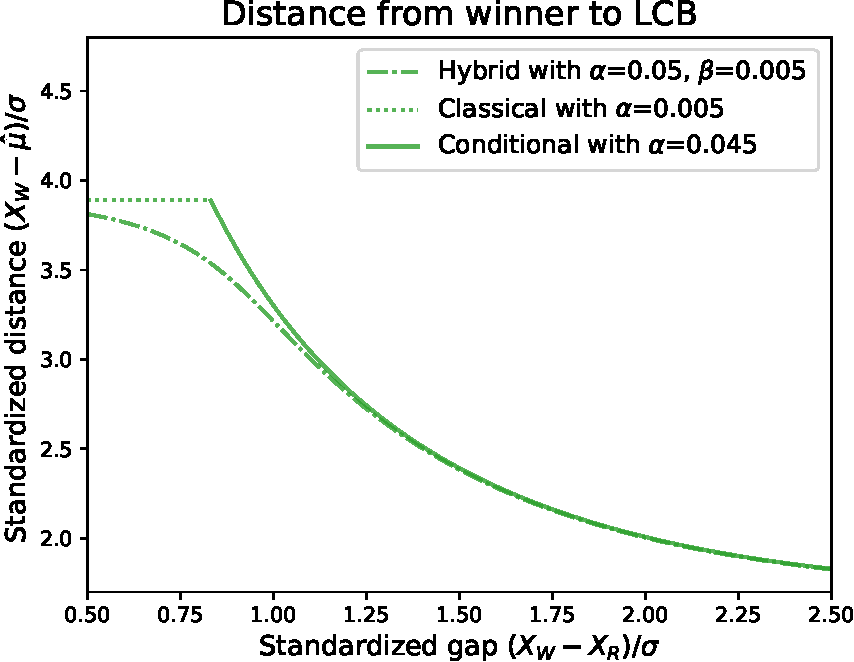
\includegraphics[width=\textwidth]{fig/hyb_dist_to_winner_n=100.pdf}
        \caption*{(b) $n=100$}
    \end{minipage}
    \hfill
    \hspace{0.01\textwidth}
    \begin{minipage}{0.32\textwidth}
        \centering
        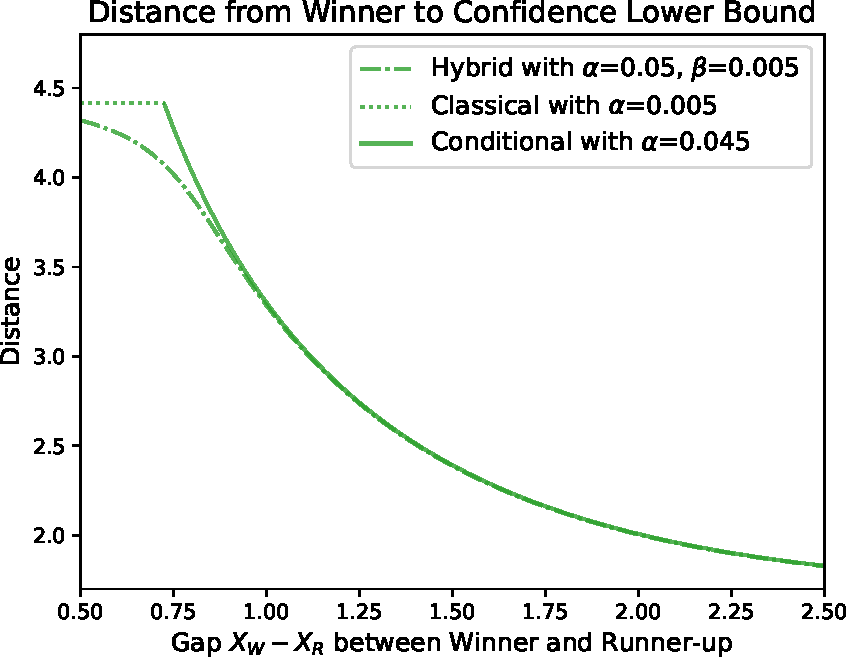
\includegraphics[width=\textwidth]{fig/hyb_dist_to_winner_n=1000.pdf}
        \caption*{(c) $n=1000$}
    \end{minipage}
    \caption{ For $n=10$ (left), $n=100$ (middle), and $n=1000$ (right) the distance between the hybrid LCB to the winner (dash-dot line) and union bound LCB to the winner (dotted and solid line) with $\alpha=0.05$ and $\beta=0.005$ plotted as a function of the gap between the winning and runner-up observation.}
    \label{fig:hybrid_union}
\end{figure}

As discussed earlier the hybrid cutoff \eqref{eq:hybrid_cutoff_thm} is strictly larger than the union bound cutoff \eqref{eq:union_bound_cutoff} when $p_{(1)} > \beta_n$. Thus, both procedures reject when $p_{(1)} \leq \beta_n$. When $p_{(1)} > \beta_n$, the hybrid procedure rejects but the union bound does not whenever  
\begin{equation*}
    p_{(1)} \in \bigg((\alpha - \beta)p_{(2)},  \frac{(\alpha - \beta)}{1-\beta}p_{(2)} + \left(1 -  \frac{(\alpha - \beta)}{1-\beta}\right)\beta_n \bigg]
\end{equation*}
When $p_{(2)} = 1$ and $n=1$, the length of the interval is $\beta$, which is the largest it can possible be. Thus, in the case where we can have additional rejections, the hybrid cutoff is never more than $\beta$ plus the union bound cutoff. \cite{Andrews2023} suggests taking $\beta=\alpha/10$, so when $\alpha = 0.05$, for example, $\beta=0.005$ is quite small. 

Still, this is not a precise statement about power gain. The computations required to compute the power gain analytically are messy, so instead we gauge the power gain via simulation. We sample data $X \sim N(\mu, I_n)$ for $n=10$ and attempt to reject the winning null $H_W: \mu_W \leq 0$ where $W = \argmin_{i \in [n]} 1 - \Phi(X_i)$ is the index of the smallest p-value $p_i = 1-\Phi(X_i)$.  

We choose $n=10$ because it is a reasonably small dimension size where one may apply hybrid inference (e.g., the main example from \cite{Andrews2023} has $n=13$). Let $R$ denote the index of the runner-up (second largest observation). For the dimensions  $n=10, 100, 1000$, \Cref{fig:hybrid_union} 
compares the distance from the winner $X_W$ the hybrid LCB and the union bound LCB. As illustrated in the plot, the (small) benefit of hybrid inference dissapates as the dimension of the problem increases. This is because conditioning on the good event has less and less of an effect as $n$ grows. 

Our simulation results indicate that hybrid inference typically results in a fairly small power gain. We consider two simulated settings: \newline 

\noindent \textbf{Needle in a haystack: } First, we consider a needle in the haystack setting where $\mu_1 > 0$ and all the other $\mu_i$ for $ i\neq 1$ are set to $\mu_2$. We try $\mu_2 = -2, 0, 2$. The power comparison is ploted in \Cref{fig:hybrid_union_power}. Whenever we truly have a needle in the haystack problem, i.e., $\mu_1 > \mu_2$, hybrid inference results in essentially no power gain. The only setting where we see some gain (up to around $0.05$) is when $\mu_2 > \mu_1$. In this setting  we actually have a dense alternative (many small signals). We expect the top two p-values to be close to each other, so conditional methods should perform poorly. The union bound approach indeed performs essentially identically to the level $\beta$ classical test (not pictured). Hybrid, however, manages to eke out some additional power. Both methods pale in comparison to the level $\alpha$ classical test however, which would achieve power $>0.95$ throughout the whole plot (not pictured).For various values of $\sigma_1$ and $\sigma_2$ which we assume are known, we also tried re-running the experiments with  $X_1 \sim N(\mu_1, \sigma_1^2)$ and $X_i \sim N(\mu_2, \sigma_2^2)$ when $i > 1$. The results were not appreciably different.  \newline 

\noindent \textbf{Two possible signals: } Seeing as the hybrid and union bound approaches both reject based on the winning and running-up p-value, we ran a simulation for all pairs $\mu_1, \mu_2 \in \{-3, -2.9, \dots, 2.9, 3 \}$ with $\mu_1 > \mu_2$ and $\mu_1 > 0$. We forcibly set $\mu_i = -\infty$ for $i > 2$. For each setting we ran $N=10000$ to get an empirical estimate of power for each method. Across the $1492$ simulated settings, the median emprical power increase from hybrid was $\approx 0.003$, the $90$th percentile empirical power increase was $\approx 0.023$ and the maximum empirical power increase was $\approx 0.042$. As the results indicate, the power increases from hybrid were negligble for most settings. We also re-ran the same simulations but sampled $X_1 \sim N(\mu, \sigma_1^2)$ and $X_2 \sim N(\mu, \sigma_2^2)$ for various values of $\sigma_1$ and $\sigma_2$, which we assume are known. The results were not appreciably different, and, if anything, the difference in power was notably smaller for some values of $\sigma_1$ and $\sigma_2$.  


\begin{figure}
    \centering
    \hspace{-0.035\textwidth}
    \begin{minipage}{0.32\textwidth}
        \centering
        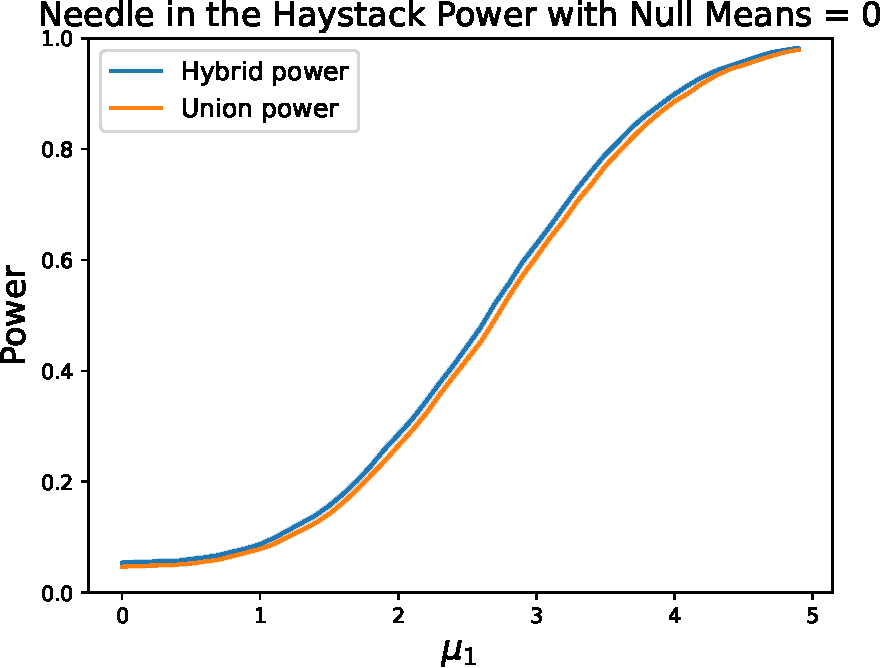
\includegraphics[width=\textwidth]{fig/hybrid_vs_union_null=0.pdf}
        \caption*{(a) $\mu_2 = -2$}
    \end{minipage}
    \hfill
    \hspace{0.01\textwidth}
    \begin{minipage}{0.32\textwidth}
        \centering
        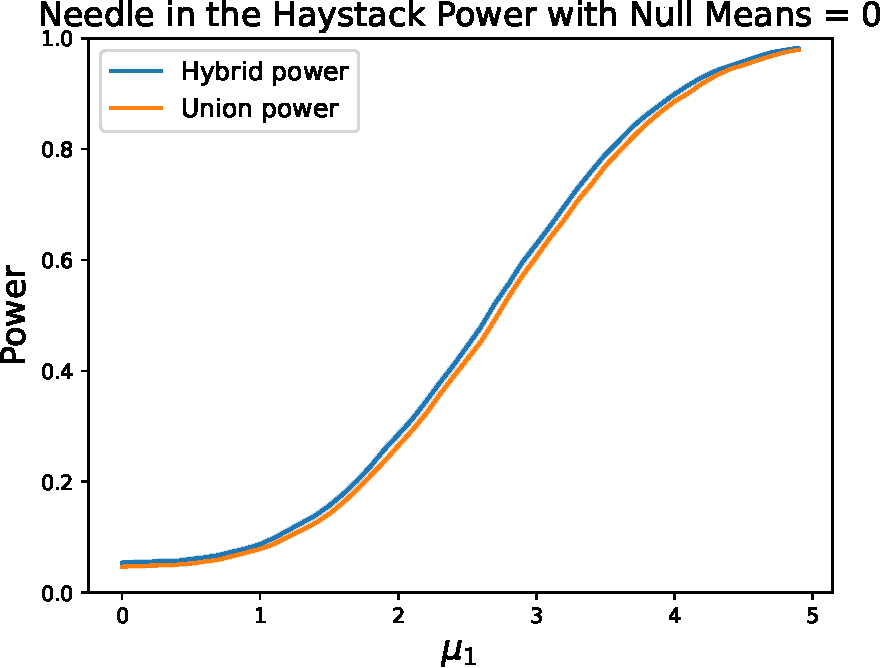
\includegraphics[width=\textwidth]{fig/hybrid_vs_union_null=0.pdf}
        \caption*{(b) $\mu_2 = 0$}
    \end{minipage}
    \hfill
    \hspace{0.01\textwidth}
    \begin{minipage}{0.32\textwidth}
        \centering
        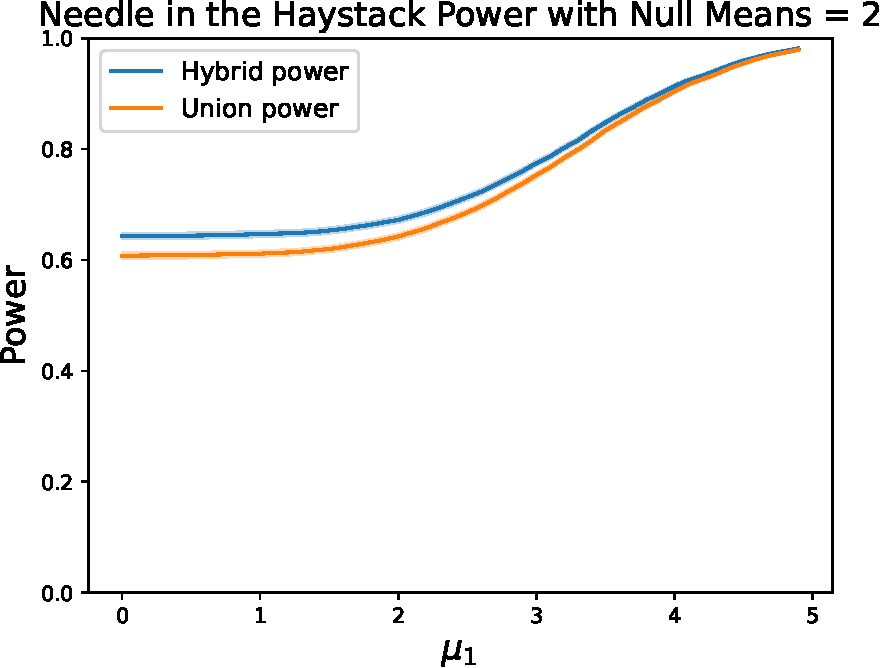
\includegraphics[width=\textwidth]{fig/hybrid_vs_union_null=2.pdf}
        \caption*{(c) $\mu_2=2$}
    \end{minipage}
    \caption{ For $\mu_2=0$ (left), $\mu_2=-0.5$ (middle), and $\mu_2=-1$ (right) the empirical power over $N=10^4$ trials of the hybrid inference approach versus the union bound approach for the needle in the haystack alternative. One standard error bands are also plotted. For the most part, they are so small that they are hardly visible.  }
    \label{fig:hybrid_union_power}
\end{figure}

\subsection{p-value Adjustment for Exponential Families}
\label{sec:rank_verficiation_adj_appdx}

Suppose $p$ is a p-value for the null $H_0$ that is selectively dominant given $Z$ and we select $p$ to use for inference according to the selection function 
    \begin{equation*}
        s(x, z) = 
        \begin{cases} 
        1 & \text{if } x < q^+(z), \\
        \frac{1}{N(z)} & \text{if } x \in [q^+(z), q(z)], \\
        0 & \text{otherwise},
        \end{cases},
    \end{equation*}
Then the adjusted p-value \eqref{eq:adjustment} is given by 
\begin{equation*}
    p_{adj} = \frac{\int_0^p s(x, Z) dx }{\int_0^1 s(x, Z)dx} = 
        \begin{cases} 
        \frac{p}{q^{+}(Z) + \frac{1}{N(Z)}(q(Z) - q^{+}(Z)) }  & \text{if } p  < q^+(Z), \\
        \frac{q^{+}(Z)+ \frac{1}{N(Z)}(p - q^{+}(Z))}{q^{+}(Z) + \frac{1}{N(Z)}(q(Z) - q^{+}(Z)) } & \text{if } p \in [q^+(Z), q(Z)], \\
        \end{cases},
\end{equation*}
which can be re-written as 
\begin{equation*}
   p_{adj} = \frac{p - (1-\frac{1}{N(Z)})(p - q^+(Z))_+ }{q^+(Z) + \frac{1}{N(Z)}(q^+(Z) - q(Z))}.
\end{equation*}
This is sufficient to imply the claim from the main text. 

\subsection{Smallest p-value and the Winner}
\label{sec:small_p_val_appdx}

We give a quick example showing that, in parameteric settings, we cannot always use the smallest p-value to determine the winner. Suppose that $X_1 \sim N(\mu_1, \sigma_1^2)$ and $X_2 \sim N(\mu_2, \sigma_2^2)$ with the $\mu_i$ unknown but $\sigma_i$ known. The UMP p-value for testing the null $H_{0, i}^{\mu_0}: \mu_i \leq \mu_0$ is given by $p^{\mu_0}_i = 1- \Phi(\frac{X_i - \mu_0}{\sigma})$. Suppose that $\sigma_1 = 1$, $\sigma_2 = 3$ and we observe $X_1 = 1$ and $X_2=2$. Then
\begin{equation*}
    p^0_1 = 1 - \Phi(1) < 1 - \Phi(2/3) = p^0_2
\end{equation*}
but 
\begin{equation*}
    p^1_1 = 1 - \Phi(0) > 1 - \Phi(1/3) = p^0_2.
\end{equation*}

\subsection{Comparing Selection Functions}
\label{sec:publication_bias_appdx}

Consider a selectively dominant p-value $p$ for the null $H_0$ that is valid conditional on $Z$, and two binary selection variables $S_1 \in {0, 1}$ and $S_2 \in {0, 1}$ whose joint relationships with $p$ are governed by two different selection functions:
\begin{equation*}
    s_1(x, z) = P(S_1 = 1 | p=x, Z=z),
\end{equation*} 
\begin{equation*}
    s_2(x, z) = P(S_2 = 1 | p=x, Z=z)
\end{equation*} 
Sometimes, if the selection function $s_1(x, z)$ is harsher than the other $s_2(x, z)$ then using \Cref{thm:adjustment}'s adjusted p-value under $s_1(x, z)$ maintains error control even when $p$ is selected according to $s_2(x, z)$. In particular, whenever
\begin{equation*}
    p_{adj, 2} =  \frac{\int_0^p s_2(x, Z) dx }{\int_0^1 s_2(x, Z) dx}  \leq \frac{\int_0^p s_2(x, Z) dx }{\int_0^1 s_2(x, Z) dx} = p_{adj, 1}
\end{equation*}
we have from \Cref{thm:adjustment} that 
\begin{equation*}
    P_{H_0}(p_{adj, 1}  \leq \alpha \mid S_2 = 1 ) \leq   P_{H_0}(p_{adj, 2}  \leq \alpha \mid S_2 = 1 )  \leq \alpha.
\end{equation*}

One example that is relevant to our publication bias application is where $s_1(x) = I_{x \leq \alpha}$ and $s_2(x)$ is any function that takes some constant value $c \in [0, 1]$ (we make no assumptions about what values $s_2(x)$ takes outside of $(0, \alpha]$). The adjusted p-value $p_{adj, 1} = p/\alpha$ remains unchanged if we take $s_1(x) = cI_{x \leq \alpha}$, so instead (scaling the selection function by a positive constant does not change the adjustment), so intstead imagine working with this selection function. Then we see that 

\begin{align*}
    \frac{\int_0^p s_2(x, Z) dx }{\int_0^1 s_2(x, Z) dx}  \leq \frac{\int_0^p s_1(x, Z) dx }{\int_0^1 s_1(x, Z) dx} &\iff  \frac{\int_0^1 s_2(x, Z) dx}  {\int_0^p s_2(x, Z) dx }\geq \frac{\int_0^1 s_1(x, Z) dx}{\int_0^p s_1(x, Z) dx }\\
    &\iff 1 + \frac{\int_p^1 s_2(x, Z) dx}  {\int_0^p s_2(x, Z) dx }\geq 1 + \frac{\int_p^1 s_1(x, Z) dx}{\int_0^p s_1(x, Z) dx }\\
    &\iff \frac{\int_p^1 s_2(x, Z) dx}  {\int_0^p s_2(x, Z) dx }\geq \frac{\int_p^1 s_1(x, Z) dx}{\int_0^p s_1(x, Z) dx }
\end{align*}
Examine the last inequality. When $p > \alpha$ the numerator of the right-hand side of is $0$, so it must be true. If $p \leq \alpha$, then the denominators of both sides of the last inequality are equal but the numerator of the left-hand side is at least that of the numerator of the right-hand side, which is at most $c(\alpha - p)$. Therefore, the entire string of inequalities, including the first one, is true, implying that $p_{adj, 2} \leq p_{adj, 1}$. 

Now we briefly consider the case that $c=0$, so $s_2(x)$ is $0$ on the interval $[0, \alpha]$. It is clear for $p$ such that $\int_0^p s_2(x)dx = 0$ that the first inequality is true (the remaining inequalities are no longer well defined since they require dividing by zero). If $p$ is such that  $\int_0^p s_2(x)dx > 0$, then we must have $p > \alpha$, so again the last inequality is true by the same reasoning as above (now the remaining inequalities are well defined). Again, we find that $p_{adj, 2} \leq p_{adj, 1}$.

\section{Scratch-work}

\subsection{Data Carving for File Drawer Adjustment}

We have two data samples $X_1 \sim N(\mu, 2)$ and $X_2 \sim N(\mu, 2)$ that are independent and want to test $H_0 : \mu \leq 0$. Suppose we only do inference because we observed that $X_1  > t$ for some threshold $t$. If we consider the p-value $p = 1 - \Phi((X_1 + X_2)/2  )$, then our selection function is given by 

\begin{align*}
    s(x) &= P( X_1 > t | p = x ) \\
         &=  P( X_1 > t | \frac{X_1 + X_2}{2} =  \Phi^{-1}(1 -x) )\\
         &= 1 - \Phi(t - \Phi^{-1}(1 - x))
\end{align*}

where we have used that 

\begin{equation*}
    \begin{bmatrix}
    X_1 \\ \frac{X_1 + X_2}{2}
    \end{bmatrix} \sim N \left(\begin{bmatrix}
        \mu \\ \mu
        \end{bmatrix}, \begin{bmatrix}
            2  & 1 \\ 1 & 1
            \end{bmatrix} \right)
\end{equation*}

\begin{equation*}
    X_1 | \frac{X_1 + X_2}{2} = y \sim N(y, 1)
\end{equation*}


Thus our corrected p-value is given by 

\begin{equation*}
    p_{adj} = \frac{\int_0^p  1 - \Phi(t - \Phi^{-1}(1-x) )   dx }{\int_0^1 1 - \Phi(t - \Phi^{-1}(1-x) ) dx}
\end{equation*}
\begin{equation*}
    p_{adj} = \frac{\int_{\bar{X}}^{\infty} \phi(z) (1 - \Phi(t - z))   dz }{\int_{-\infty}^{\infty} \phi(z) (1 - \Phi(t - z))  dz } = \frac{\int_{\bar{X}}^{\infty} \phi(z) (1 - \Phi(t - z))   dz }{1 - \Phi(t/\sqrt{2})   }
\end{equation*}

Letting $Z$ and $Y$ be independent standard normal random variables and fixing some constant $a$, this adjusted p-value is just 
\begin{equation*}
   p_{adj} = \frac{P(Z + Y > t, Z > a)}{P(Z + Y > t)} = P(Z > a | Z + Y > t)
\end{equation*}
for $a = \bar{X}$. Letting $W = Z + Y$ we can write $Z = \frac{1}{2}W +\epsilon$ where $\epsilon$ is independent of $W$. This gives us 
\begin{equation*}
    p_{adj} = P(\frac{1}{2} W + \epsilon > a | W > t) = E[P(W > 2(a - \epsilon)| W > t, \epsilon)| W > t ] = E[P(W > 2(a - \epsilon)| W > t, \epsilon)]
\end{equation*}
Then the fact that $p_{adj}$ is monotone non-decreasing in $t$ follows from the fact that $P(W > c | W > t)$ is monotone non-decreasing in $t$ for every constant $c$:
\begin{equation*}
{P(W > c |W >t)} = \begin{cases} 
\frac{P(W > c)}{P(W > t)} & \text{if } c \geq t \\
1 & \text{if } c < t 
\end{cases}
\end{equation*}



\section{Selecting Multiple p-Values for Inference}
\label{sec:multiple_p_vals_appdx}

In this appendix, we generalize our selective dominance framework to allow us to select multiple p-values for inference. We only do this generilization 

Suppose we have $n$ ndependent and selectively dominant p-values for the nulls $H_{0, i}$. We imagine conditioning on some collection of them, which, without loss of generality, we can take to be $Z = (p_{k+1}, \dots, p_n)$. Note that, due to independence, conditioning on $Z$ does not change the distribution of $p_j$. Thus, the $p_j$ remain p-values under the nulls $H_{0, j}$ that are independent. Now, for $1 \leq j \leq k$, we consider $k$ binary selection random variables $S_j \in \{0, 1\}$, where $S_j = 1$ when $p_j$ is selected. The relationship between $p_j$, $Z$, and $S_j$ is governed by the selection function 
\begin{equation*}
    s_j(x, z) = p(S_j = 1 | p_j = x, Z=z)
\end{equation*} 
Supposing that $U$ is a uniform random variable that has a uniform distribution given $Z$, we can imagine selecting $U$ using the same selection functions. I.e., we can imagine that a binary selection variable $S_j \in {0, 1}$ whose joint distribution with $U$ is governed by 
\begin{equation*}
    P(S_j = 1| U = x, Z = z) = s(x, z)
\end{equation*}
Then the machinery from \Cref{sec:dominance} tells us that 
\begin{equation*}
    p_{adj, j} = F_{U |Z, S_j = 1}(p_j) = \frac{\int_0^{p_j} s_j(x, Z)dx }{\int_0^1 s_j(x, Z)dx}
\end{equation*}
is p-value (it stochastically dominates the uniform distribution under the null) conditional on $Z$ and selection. 

We will further assume that the selection happens independently, i.e., 
\begin{equation*}
    P(S_1 = 1, \dots, S_k = 1 \mid p_1, \dots, p_k, Z) = \prod_{j = 1}^k P(S_j = 1 \mid p_j, Z)
\end{equation*} 
By taking expectations conditional on $Z$ with respect to both sides, we find that the $S_j$ are independent given $Z$:
\begin{align*}
    P(S_1 = 1, \dots, S_k = 1 \mid Z) &= E[P(S_1 = 1, \dots, S_k = 1 | p_1, \dots, p_k, Z) \mid Z] \\
    &= E \left[\prod_{j = 1}^k P(S_j = 1 | p_j, Z) \;\middle|\; Z\right]\\
    &= \prod_{j=1}^k E[P(S_j = 1 | p_j, Z)]\\
    &= \prod_{j=1}^k P(S_j = 1 | Z)
\end{align*}
where we have used that the $p_j$ are conditionally independent given $Z$ to move the expectation inside the product. Finally, conditional on $Z$ and all the selections $S_j=1$, the adjusted p-values $p_{adj, j}$ are all independent of one another. 
\begin{equation*}
    P(p_{adj, 1} \in A_1, \dots, p_{adj, k} \in A_k \mid Z, S_1 = 1, \dots, S_k = 1) = \prod_{j=1}^k P(p_{adj, j} \in A_j \mid Z, S_j = 1)
\end{equation*}
This can be confirmed via Bayes rule:
\begin{align*}
    &P(p_{adj, 1} \in A_1, \dots, p_{adj, k} \in A_k \mid Z, S_1 = 1, \dots, S_k = 1) \\
    &= \frac{p(p_{adj, 1} \in A_1, \dots, p_{adj, k} \in A_k, | Z) P( S_1 = 1, \dots, S_k = 1 \mid Z, p_{adj, 1} \in A_1, \dots, p_{adj, k} \in A_k)  }{P(S_1=1, \dots, S_k = 1 | Z)}\\
    &= \frac{a + b}{c}
\end{align*}

\section{Selective Dominance and One-Sided Testing}

In this appendix, we establish the selective dominance property for UMP p-values in MLR familes and UMPU p-values in exponential families. We also show that in these cases, the adjusted p-value from \Cref{thm:adjustment} is monotone in the parameter, under suitable conditions. Throughout the appendix, we draw from the discussion and proof strategy in Appendix B.1 of \cite{Lei}.

\subsection{MLR Families}

We consider a parametric family $P_{\theta}$ parameterized by a real parameter $\theta \in R$ such that each $P_{\theta}$ has density $p_{\theta}(x)$ with respect to some carrier measure $\mu$. We will suppose that these densities share support (i.e., for any two $\theta$ and $\theta'$ we have $p_{\theta}(x) > 0 \iff p_{\theta'}(x)> 0$). Further, we suppose that for any $\theta < \theta'$, the likelihood ratio $p_{\theta'}(x)/p_{\theta}(x)$ is a monotone non-decreasing function of some real-valued function $T(x)$ on this support (i.e, for any $x_1 \leq x_2$ with $p_{\theta}(x_1), p_{\theta}(x_2) > 0$, we have $p_{\theta'}(x_1)/p_{\theta}(x_1) \leq p_{\theta'}(x_2)/p_{\theta}(x_2)$). 

%To be fully general we only define the likelihood ratio when at least one of the numerator and denominator are non-zero and let it equal $\infty$ when the denominator is zero.

Recall that for a testing problem, the critical function $\phi(x)$ (see \cite[Section 3.1]{Lehmann}) tells us the probability of rejecting the null having observed data $x$, so $\phi(X) = P(\text{reject } H_0 | X)$. From Theorem 3.4.1 of \cite{Lehmann} we know the test governed by the critical function 
\begin{equation}
    \label{eq:mlr_test}
    \phi(x) = \begin{cases}
        1 &\text{if } T(x) > C  \\
        \gamma &\text{if } T(x) = C  \\
        0 & \text{otherwise }
    \end{cases}
\end{equation}
is UMP for testing $H_0 : \theta \leq \theta_0$ against the alternatives $H_a : \theta > \theta_0 $ so long $C$ and $\gamma$ satisfy
\begin{equation}
    \label{eq:constraint}
    P_{\theta_0}(T(X) > C) + \gamma P_{\theta_0}(T(X) = C) = \alpha.
\end{equation}
Denote the left-continuous survival function of $T(X)$ and its righthand limit under $P_{\theta_0}$ as
\begin{equation*}
    G(t) = P_{\theta_0}(T(X) \geq t) \qquad G^+(t) = \lim_{u \downarrow t} G(u).
\end{equation*}
Since $G(t)$ is a monotone non-increasing function, we can also define its generalized inverse 

\begin{equation*}
    G^{-1}(z) = \inf \{ t : G(t) \leq z\},
\end{equation*}

\Cref{lem:setting_constants} gives a natural way to set $C$ and $\gamma$ in \Cref{eq:mlr_test} to get an UMP test. 

\begin{lemma}[An UMP test]
    \label{lem:setting_constants} Adopting the convention that $0/0 = 0$, taking $C = G^{-1}(\alpha)$ and $\gamma = (\alpha - G^+(C))/(G(C) - G^+(C))$
    in \Cref{eq:mlr_test} gives an UMP test.
\end{lemma}

\begin{proof}
    At continuity points $t$ of $G(\cdot)$, we have $G(G^{-1}(t)) = t$ and also $P(T(X) = t) = 0$. Thus, if $C = G^{-1}(\alpha)$ is a continuity point of $G(\cdot)$, then $G^+(C) = P_{\theta_0}(T(X) > C) = P_{\theta_0}(T(X) \geq C) = G(C) = \alpha$ and $\gamma=0$, so the constraint \eqref{eq:constraint} is immediately satisfied. 

    If $C = G^{-1}(\alpha)$ is not a continuity point of $G(\cdot)$, then $G(C) - G^+(C) > 0$ and the constraint \eqref{eq:constraint} is also immediately satisfied. To ensure that we still have a valid test, however, we need $\gamma \in [0, 1]$. This is true so long as $\alpha \in [G^{+}(C), G(C)]$. We know that $G(t) \leq \alpha$ for any $t > C$, so $G^{+}(C) \leq \alpha$. If $G(C) < \alpha$, then we could find some $t^{-} < C$ such that $G(C) < \alpha$ by left-continuity, but this would contradict that $C = G^{-1}(\alpha)$, finishing the proof. 
\end{proof}

Letting $U_{aux} \sim \text{Unif}([0, 1])$ be auxiliary randomness that is independent of $X$, a simple way to instantiate the test from \Cref{lem:setting_constants} is to reject whenever $T(X) > C$ or when $T(X) = C$ and $U_{aux} \leq \gamma$. \Cref{lem:fuzzy} explains how this is the same as rejecting when the p-value, termed as a fuzzy p-value in \cite{Geyer}, 
\begin{equation}
    \label{eq:mlr_p_val}
    p = G^+(T(X)) + U_{aux}(G(T(X)) - G^+(T(X))) 
\end{equation}
is at most $\alpha$. 

\begin{lemma}[Fuzzy p-value is UMP]
    \label{lem:fuzzy}
    Rejecting $H_0: \theta \leq \theta_0$ when the fuzzy p-value \eqref{eq:mlr_p_val} is at most $\alpha$ instantiates the test from \Cref{lem:setting_constants}, and is therefore UMP. 
\end{lemma}

\begin{proof} We rewrite 
    \begin{equation*}
        p = (1 - U_{aux})G^+(T(X)) + U_{aux} G(T(X))
    \end{equation*}
    and consider four  cases. 
    \begin{itemize}
        \item If $t < G^{-1}(\alpha)$ then we can find some $t^+ > t$ such that $G(t^+) > \alpha$. Thus $G(t) \geq G^{+}(t) > \alpha$. So $p > \alpha$ whenever $T(X) < G^{-1}(\alpha)$ 
        \item If $t = G^{-1}(\alpha)$ and $G^{-1}(\alpha)$ is a continuity point of $G(\cdot)$, then $G^{+}(t) = G(t) = \alpha$. Thus, in this case $p \leq \alpha$ whenever $T(X) = G^{-1}(\alpha)$ and $U_{aux} \leq  \frac{\alpha - G^+(G^{-1}(\alpha))}{G(G^{-1}(\alpha)) - G^+(G^{-1}(\alpha))} = \infty$. 
        \item If $t = G^{-1}(\alpha)$ and $G^{-1}(\alpha)$ is not a continuity point of $G(\cdot)$, then we must have that $G(t) - G^+(t)  > 0$. Also by right continuity we have $G(t) \geq \alpha$ and by how $G^{-1}(\cdot)$ is defined we have $G^+(t) \leq \alpha$. In this case $p \leq \alpha$ also whenever $T(X) = G^{-1}(\alpha)$ and $U_{aux} \leq  \frac{\alpha - G^+(G^{-1}(\alpha))}{G(G^{-1}(\alpha)) - G^+(G^{-1}(\alpha))}$. 
        \item If $t > G^{-1}(\alpha)$ then $G^+(t) \leq G(t) \leq \alpha$. So $p \leq \alpha$ whenever $T(X) > G^{-1}(\alpha)$. 
    \end{itemize}


    This implies the following set equalities:

    \begin{align*}
        \{p \leq \alpha \} &= \{T(X) > G^{-1}(\alpha) \} \cup \left\{T(X) =  G^{-1}(\alpha), U_{aux} \leq \frac{\alpha - G^+(G^{-1}(\alpha))}{G(G^{-1}(\alpha)) - G^+(G^{-1}(\alpha))} \right\}\\
                           &= \{T(X) > C \} \cup \left\{T(X) =  C, U_{aux} \leq \gamma \right\}\\
    \end{align*}

\end{proof}


\Cref{lem:uniform} shows that $p \sim \text{Unif}([0, 1])$ under $P_{\theta_0}$, which will be useful for us later. 

\begin{lemma}[Fuzzy p-value is uniform at null boundary]
    \label{lem:uniform}
    Under $P_{\theta_0}$, the p-value \eqref{eq:mlr_p_val} has a $\text{Unif}([0, 1])$ distribution.
\end{lemma}

\begin{proof}

Using the set equality from \Cref{lem:fuzzy} but replacing $\alpha$ with $z \in (0, 1)$, we find

\begin{align*}
        &P_{\theta_0}(G^+(T(X)) + U_{aux}(G(T(X)) - G^+(T(X))) \leq z)\\
        &= P_{\theta_0}(T(X) > G^{-1}(z)) + P_{\theta_0}\left(T(X) = G^{-1}(z),  U \leq \frac{z - G^+(G^{-1}(z))}{G(G^{-1}(z)) - G^{+}(G^{-1}(z))}\right)\\
        &= P_{\theta_0}(T(X) > G^{-1}(z)) + P_{\theta_0}(T(X) = G^{-1}(z)) P_{\theta_0}\left(U \leq \frac{z - G^+(G^{-1}(z))}{G(G^{-1}(z)) - G^{+}(G^{-1}(z))}\right)\\
        &=G^+(G^{-1}(z)) + (G(G^{-1}(z)) - G^{+}(G^{-1}(z))) \cdot \frac{z - G^+(G^{-1}(z))}{G(G^{-1}(z)) - G^{+}(G^{-1}(z))}\\
        &= z.
    \end{align*}

\end{proof}

Now we can show that $p$ is a selectively dominant p-value for testing the null $H_0: \theta \leq \theta_0$. In what follows, we consider some fixed $\theta \leq \theta_0$ and prove some facts that allow us to relate the distribution of $T(X)$ under $P_{\theta_0}$ to its distribution under $P_{\theta}$.

\begin{lemma}[Distribution of $T(X)$]
    \label{lem:stan_machine}
    Let $g_{\theta}(T(x))$ be a non-increasing function that equals the likelihood ratio $p_{\theta}(x)/p_{\theta_0}(x)$ on the support and 
    \begin{equation*}
        \nu(A) = \int I(T(x) \in A) p_{\theta_0}(x) \mu(dx)
    \end{equation*}
    be the meausre of $T(X)$ under $X \sim P_{\theta_0}$. Then 
    \begin{equation*}
        P_{\theta}(T(X) \in A) = \int_A g_{\theta}(t) \nu(dt)
    \end{equation*}
\end{lemma}

\begin{proof}
We know that 
\begin{align*}
    P_{\theta}(T(X) \in A) = \int I(T(x) \in A) p_{\theta_0}(x)g_{\theta}(T(x)) \mu(dx), 
\end{align*}
so we need to show that 
\begin{equation}
    \label{eq:stan_machine_to_show}
    \int I(T(x) \in A) p_{\theta_0}(x) g_{\theta}(T(x)) \mu(dx) =  \int_A g_{\theta}(t) \nu(dt)
\end{equation}
If $g_{\theta}(T(x)) = I(T(x) \in A')$ happens to be an indicator then \eqref{eq:stan_machine_to_show} holds. Therefore, we can apply the standard machine (see the discussion after Equation 42 in \cite{Lei}) to show that \eqref{eq:stan_machine_to_show} holds for all non-negative functions $g_{\theta}(\cdot)$.  
\end{proof}


\begin{lemma}[Distribution of $(T(X), U_{aux})$]
    \label{lem:pi_lambda}
    If $\omega$ denotes the product measure of $\nu$ and Lesbesgue measure $\lambda$ on $[0, 1]$, i.e., the distribution of $(T(X), U_{aux})$ under $P_{\theta_0}$, then 
    \begin{equation}
    \label{eq:joint_dist}
        P_{\theta}((T(X), U) \in B) = \int_{B} g_{\theta}(t) \omega(dt, du)
    \end{equation}
\end{lemma}

\begin{proof}
    We will first argue that \eqref{eq:joint_dist} holds for any $B$ which is a product set $A_1 \times A_2$. We can futher reduce to the case that $g_{\theta}(T(x)) = I(T(x) \in A_1')$ is an indicator. Then we see using our previous lemma that 
    \begin{align*}
        P_{\theta}((T(X), U_{aux}) \in A_1 \times A_2) &= P_{\theta}(T(X) \in A_1)P(U_{aux} \in A_2)\\
                                          &= \int_{A_1} g_{\theta}(t) \nu(dt) \cdot \int_{A_2} \lambda(du)\\
                                          &= \int_{A_1 \cap A_1'} \nu(dt) \cdot \int_{A_2} \lambda(du)\\
                                          &= \int_{A_1 \cap A_1' \times A_2} \omega(dt, du)\\
                                          &= \int_{A_1 \times A_2} g_{\theta}(t)\omega(dt, du)
    \end{align*}
    To handle the case of general $g_{\theta}(\cdot)$ we can again simply apply the standard machine. 
    
    The full result then follows from an application of the $\pi-\lambda$ theorem: the set of $B$ for which \eqref{eq:joint_dist} holds is a $\lambda$-system, and \eqref{eq:joint_dist} holds for every set in the $\pi$ system of all product sets $B = A_1 \times A_2$. 
\end{proof}

Note that our p-value $p$ is a deterministic function of $T(X)$ and $U_{aux}$:
\begin{equation*}
    p = m(T(X), U_{aux}) \qquad m(t, u) = G^+(t) + u(G(t) - G^+(t)).
\end{equation*}
As such, we sometimes write our selection function as a function of $T(X)$ and $U_{aux}$:
\begin{equation*}
    s(t, u) = s(m(t, u)). 
\end{equation*}
We use this abuse of notation in our next lemma, which characterizes the conditional distribution of $T(X)$ given selection.

\begin{lemma}[Distribution of $(T(X), U_{aux})$ given selection]
    For any selection function $s(x)$ under which $p$ has a positive probability of selection under $P_{\theta}$, 
    \begin{equation*}
        P_{\theta}((T(X), U_{aux}) \in B| S = 1 ) = \frac{\int_{B} g_{\theta}(t)s(t, u) \omega(dt, du)}{ \int g_{\theta}(t) s(t, u) \omega(dt, du) }
    \end{equation*}
\end{lemma}

\begin{proof} First note that
    \begin{equation*}
        P_{\theta}( (T(X), U_{aux}) \in B | S= 1 ) = \frac{P_{\theta}((T(X), U_{aux}) \in B, S = 1) }{P_{\theta}(S = 1)}.
    \end{equation*} 
    Thus it suffices to show for any set $B$ that 
    \begin{equation*}
        P_{\theta}( (T(X), U_{aux}) \in B,  S= 1 ) = \int_B g_{\theta}(t) s(t, u) \omega(dt, du). 
    \end{equation*} 
    By the definition of conditional expecation
    \begin{align*}
        P_{\theta}( (T(X), U_{aux}) \in B,  S= 1 ) &= E_{\theta}[E_{\theta}[ I(S=1) \mid  T(X), U_{aux}] I((T(X), U_{aux}) \in B) ]\\
                                                   &= E_{\theta}[ s(T(X), U_{aux}) I((T(X), U_{aux}) \in B) ]
    \end{align*}
    If $s(t, u) = I_{(t, u) \in B}$ is an indicator function, then the result is implied by our previous lemma. We again get the result for general selection functions $s(t, u)$ by applying the standard machine. 
\end{proof}


With these lemmas under our belt, we can show \Cref{prop:mlr_sel_dom}, the main result of this sub-section. Since $p \sim_{P_{\theta_0}} \text{Unif}([0, 1])$ by \Cref{lem:uniform}, this proposition is sufficient to imply selective dominance. 

\begin{proposition}
    \label{prop:mlr_sel_dom}
    For any selection function $s(x)$ for which $p$ has positive probability of selection under both $\theta$ and $\theta_0$,  
    \begin{equation*}
        P_{\theta}(p \leq z | S = 1)  \leq P_{\theta_0}(p \leq z | S = 1).
    \end{equation*}
\end{proposition}

\begin{proof}

Fix $z \in (0, 1)$. If $z$ is such that $P_{\theta}(p \leq z | S = 1)  = 0$ then the desired inequality is trivial. To handle the non-trival case, we note three facts from the proof of \Cref{lem:fuzzy}:
\begin{itemize}
    \item If $(t, u) \in m^{-1}([0, z])$ then $t \geq G^{-1}(z)$,
    \item If $(t, u) \in m^{-1}((z, 1])$ then $t \leq G^{-1}(z)$,
    \item The sets $m^{-1}([0, z])$ and $m^{-1}((z, 1])$ are disjoint.
\end{itemize}
Thus,
\begin{align*}
     \frac{1}{P_{\theta}(p \leq z | S = 1)} &= \frac{\int_{m^{-1}([0, 1])} g_{\theta}(t) s(t, u) \omega(dt, du) }{\int_{m^{-1}([0, z])} g_{\theta}(t) s(t, u) \omega(dt, du) }\\
                                            &= \frac{\int_{m^{-1}([0, z])} g_{\theta}(t) s(t, u) \omega(dt, du) + \int_{m^{-1}((z, 1])} g_{\theta}(t)  s(t, u)\omega(dt, du) }{\int_{m^{-1}([0, z])} g_{\theta}(t) s(t, u) \omega(dt, du) }\\
                                            &= 1 + \frac{\int_{m^{-1}((z, 1])} g_{\theta}(t) s(t, u) \omega(dt, du)}{\int_{m^{-1}([0, z])} g_{\theta}(t) s(t, u) \omega(dt, du)}\\
                                            &\geq 1 + \frac{g_{\theta}(G^{-1}(z))  \int_{m^{-1}((z, 1])}  s(t, u) \omega(dt, du)}{g_{\theta}(G^{-1}(z)) \int_{m^{-1}([0, z])} s(t, u) \omega(dt, du)} \\
                                            &= 1 + \frac{\int_{m^{-1}((z, 1])} s(t, u) \omega(dt, du)}{ \int_{m^{-1}([0, z])} s(t, u) \omega(dt, du)} \\
                                            &= \frac{1}{P_{\theta_0}(p \leq z | S = 1)}, 
\end{align*}
where to finish we have noted that $g_{\theta_0}(t) = 1$ almost eveywhere in the measure $\omega$. 
\end{proof}

\subsection{Exponential Families}

Suppose we observe data $X \in \R^m$ from an exponential family $P_{\theta}$ parameterized by $\theta \in \R^n$ i.e., under $P_{\theta}$ the data $X$ has density  
\begin{equation*}
    g_{\theta}(x) = \exp( \theta_1 T_1(x) + \dots + \theta_n T_n(x) - \psi(\theta) ) g(x) 
\end{equation*}
with respect to some carrier measure $\mu$. We consider the problem of testing $H_0: \theta_i \leq \theta_{0, i}$.

Letting $T_{-i}(X)$ be the random vector containing the $T_j(X)$ for $j \neq i$, the UMPU test $H_0: \theta_i \leq \theta_{0, i}$ is valid conditional on $T_{-i}(X)$. More specifically, Theorem 4.4.1 of \cite{Lehmann} tells us that any test of the form 

\begin{equation*}
    \label{eq:exp_fam_test}
    \phi(t_i, t_{-i}) = \begin{cases}
        1 &\text{if } t_i > C_0(t_{-i})  \\
        \gamma(t_{-i}) &\text{if } t_i = C_0(t_{-i})   \\
        0 & \text{otherwise }
    \end{cases}
\end{equation*}
where the functions $\gamma(\cdot)$ and $C_0(\cdot)$ satisfy 
\begin{equation*}
    E_{\theta_{0, i}}[\phi(T_i(X), T_{-i}(X)) | T_{-i}(X) ] = \alpha
\end{equation*}
is UMPU for testing $H_0: \theta_i \leq \theta_{0, i}$. Lemma 2.7.2 of \cite{Lehmann} tells us that the conditional distribuition of $T_{i}(X)$ given $T_{-i}(X) = t_{-i}$ admits a density 

\begin{equation*}
    g_{\theta_i, t_{-i}}(t_i) = \exp(\theta_i t_i - \tilde{\psi}(\theta_i))  
\end{equation*}
with respect to a base measure $\mu_{t_{-i}}$. This density has an MLR in $t_i$ (to be specific, we are imagining observing samples $T_i(X)$ from the distribution conditional on $T_{-i}(X)$ and the map $T(\cdot)$ from the previous sub-section is actually the identity). Hence, a concrete UMPU test is to just run our UMP test from the previous section using the conditional distribution given $T_{-i}(X) = t_{-i}$. In particular, our work from the previous section, implies that it is UMPU to reject when the p-value


The p-value 
\begin{equation}
    \label{eq:ump_exp_fam}
    p = G^{+}(T_i|T_{-i}) + U_{aux}(G(T_i|T_{-i}) - G^{+}_i(T_i|T_{-i})),
\end{equation}
where 
\begin{equation*}
    G(t_i | t_{-i}) = P_{\theta_0}(T_i \geq t | T_{-i} = t_{-i}) \qquad G^{+}(t) = \lim_{u \downarrow t}(T_i \geq t | T_{-i} = t_{-i} ),
\end{equation*}

is at most $\alpha$. Our work from the previous section also implies that this p-value is selectively dominant given $T_{-i}(X)$. 


\subsection{Montonicty of Adjusted MLR p-Values}

\begin{proposition}
    \label{prop:monotone_adjustment}
    Let $s_{\theta}(x)$ be a selection function such that for $\theta \leq \theta_0$, $s_{\theta_0}(x)= 0 \implies s_{\theta}(x) = 0$ and the ratio $s_{\theta_0}(x)/s_{\theta}(x)$ is non-decreasing in $x$. Then, if $p^{\theta}_{adj}$ is the adjustment from $F_{U | S_{\theta} = 1}(p^{\theta})$ then $p^{\theta}_{adj}$ is monotone non-decreasing increasing in $\theta$.  

\end{proposition}



\begin{proof}

        Fix a $t$ and $u$ and let $A_{r, s} = \{(t, u) : t > r \text{ or } t = r \text{ and } u \leq s \}$. Then it suffices to show that 
        \begin{equation*}
            \frac{ \int_{A_{t, u}}  g_{\theta}(t) s_{\theta}(t, u) \omega(dt, du)}{ \int g_{\theta}(t) s_{\theta}(t, u) \omega(dt, du)}
        \end{equation*}
        is monotone non-decreasing. Equivalently that  

        \begin{equation*}
            \frac{ \int_{A_{t, u}}  g_{\theta}(t) s_{\theta}(t, u) \omega(dt, du)}{ \int g_{\theta}(t) s_{\theta}(t, u) \omega(dt, du)} \leq \frac{ \int_{A_{r, s}} s_{\theta_0}(t, u) \omega(dt, du)}{ \int s_{\theta_0}(t, u) \omega(dt, du)}
        \end{equation*}

        If $\int_{A_{r, s}}  g_{\theta}(t) s_{\theta}(t, u) \omega(dt, du) = 0$ then the inequality is trivial. So it suffices to consider the other case and show that 

        \begin{equation*}
            \frac{ \int g_{\theta}(t) s_{\theta}(t, u) \omega(dt, du)} { \int_{A_{r, s}}  g_{\theta}(t) s_{\theta}(t, u) \omega(dt, du)} \geq \frac{ \int s_{\theta_0}(t, u) \omega(dt, du)}{ \int_{A_{r, s}} s_{\theta_0}(t, u) \omega(dt, du)}
        \end{equation*}

        \begin{equation*}
            1 + \frac{ \int_{A_{r, s}^c} g_{\theta}(t) s_{\theta}(t, u) \omega(dt, du)} { \int_{A_{r, s}}  g_{\theta}(t) s_{\theta}(t, u) \omega(dt, du)}\geq 1 + \frac{ \int_{A_{r, s}^c} s_{\theta_0}(t, u) \omega(dt, du)}{ \int_{A_{r, s}} s_{\theta_0}(t, u) \omega(dt, du)}
        \end{equation*}

        Definining $0/0 = 0$, our assumptions allow us to do the following:
        
        \begin{align*}
            \frac{ \int_{A_{r, s}^c} g_{\theta}(t) s_{\theta}(t, u) \omega(dt, du)} { \int_{A_{r, s}}  g_{\theta}(t) s_{\theta}(t, u) \omega(dt, du)} &=\frac{ \int_{A_{r, s}^c} g_{\theta}(t) s_{\theta_0}(t, u) \left( \frac{s_{\theta}(t, u) }{s_{\theta_0}(t, u)} \right) \omega(dt, du)} { \int_{A_{r, s}}  g_{\theta}(t) s_{\theta_0}(t, u) \left( \frac{s_{\theta}(t, u) }{s_{\theta_0}(t, u)} \right) \omega(dt, du)}\\
                &\geq \frac{g_{\theta}(G_{\theta}^{-1}(m(r, s))) \left( \frac{s_{\theta}(r, s) }{s_{\theta_0}(r, s)} \right)   \int_{A_{r, s}^c} s_{\theta_0}(t, u) \omega(dt, du)}{ g_{\theta}(G_{\theta}^{-1}(m(r, s))) \left( \frac{s_{\theta}(r, s) }{s_{\theta_0}(r, s)} \right)  \int_{A_{r, s}} s_{\theta_0}(t, u) \omega(dt, du)}\\
                &= \frac{  \int_{A_{r, s}^c} s_{\theta_0}(t, u) \omega(dt, du)}{   \int_{A_{r, s}} s_{\theta_0}(t, u) \omega(dt, du)}\\
        \end{align*}

\end{proof}

\subsection{Exponential Families}

\section{Proofs and Derivations}
\label{sec:proofs_appdx}

\subsection{Proof of \Cref{thm:adjustment}}
Recall we are considering a selection function such that the probability that $U$ is selected $P(S=1) = \int_0^1 s(x) dx$ is positive. The CDF of $U$ given selection is continuous because it cannot have any point masses:
\begin{equation*}
    P(U = x | S = 1) = \frac{P(U = x, S = 1)}{P(S=1)} \leq \frac{P(U = x)}{P(S=1)} =  0. 
\end{equation*}
Therefore, defining 
\begin{equation*}
    F^{-1}_{U | S=1}(t)  = \inf \{x: F_{U | S = 1}(x) > t  \}
\end{equation*}
continuity implies that $F_{U|S =1}(F^{-1}_{U | S=1}(t)) = t$ and $F_{U | S = 1}(x) \leq t \iff x \leq  F^{-1}_{U | S = 1}(t)$. Then 
\begin{equation*}
    P_{H_0}(F_{U | S = 1}(p) \leq  t | S=1) = P_{H_0}(p \leq F_{U | S = 1}^{-1}(t) | S=1) \leq P(U \leq F_{U | S = 1}^{-1}(t) | S=1) = P(F_{U|S = 1}(U) \leq t | S=1)
\end{equation*}
where we have used that $p | S=1 \succeq_{H_0} U |S=1$ to get the middle inequality. Finally 

\[P(F_{U|S = 1}(U) \leq t | S=1) = P(U \leq F_{U|S = 1}^{-1}(t) | S=1) = F_{U|S=1}(F_{U|S = 1}^{-1}(t)) = t,\]
so  $F_{U|S = 1}(U) | S = 1 \sim \text{Unif}([0, 1])$ which finishes the proof. 
 
\subsection{Proof of \Cref{thm:density}}
Let $f$ be the density of $p$ under a distribution in the null $H_0$. We start by showing that, if $f$ is non-decreasing, then $p |S =1$ dominates $U | S=1$ . Fixing a selection function $s(x)$, it suffices to show that for any $t \in [0, 1]$. 
    \begin{align*}
        &P(p \leq t | S =1) \leq P(U \leq t | S= 1)\\
        &\iff 
        \frac{\int_{0}^{t} s(x) f(x) dx }{\int_{0}^{1} s(x) f(x) dx } \leq \frac{\int_{0}^{t} s(x) dx}{\int_{0}^{1} s(x) dx } \\
    \end{align*}
If $P( p \leq t | S = 1)$ is zero then this trivially holds. Otherwise $P( p \leq t | S = 1) = \int_{0}^{t} s(x) f(x) dx  > 0$ and we see that, 
    \begin{align*}
        \frac{ \int_{0}^{1} s(x) f(x) dx }{\int_{0}^{t} s(x) f(x) dx } &= 1 + \frac{\int_{t}^{1} s(x) f(x) dx }{\int_{0}^{t} s(x) f(x) dx }\\
        &\geq 1 + \frac{f(t)\int_{t}^{1} s(x) dx }{f(t)\int_{0}^{t} s(x)  dx }\\
        &= 1 + \frac{\int_{t}^{1} s(x) dx }{\int_{0}^{t} s(x)  dx }\\
        &= \frac{ \int_{0}^{1} s(x) dx }{\int_{0}^{t} s(x)  dx },
    \end{align*}
which is sufficient to imply the claim. 

Now assuming that $f$ is continuous and non-decreasing, we can show that $p$ is not selectively dominant. In general, it suffices for there to be two points $y_1 < y_2$ such that $f$ is strictly larger in a neighborhood around $y_1$ than in a neighborhood around $y_2$, where these neighborhoods are disjoint. In particular for $\epsilon > 0$ let $N_{\epsilon}(y) = (y - \epsilon, y + \epsilon )$ be a ball around $y$. Then we need there to be $y_1$, $y_2$, $\epsilon > 0$, and some $\eta > 0$ such that, for all $z_1 \in N_{\epsilon}(y_1)$ and $z_2 \in N_{\epsilon}(y_2)$,  $z_1  < z_2$ but $f(z_2) + \eta < f(z_1) $. If $f$ is continuous and not non-decreasing, then this must be true. First define $B_{high} = \inf \{f(z_1): z_1 \in N_{\epsilon}(y_1)\}$ and  $B_{low} = \sup \{f(z_2): z_2 \in N_{\epsilon}(y_2)\}$ so $B_{high}  > B_{low}$. Then consider the selection function 
\begin{equation*}
s(x)= \begin{cases}
1 &\text{if } x \in N_{\epsilon}(y_1) \cup N_{\epsilon}(y_2) \\
0 &\text{otherwise }
\end{cases}
\end{equation*}
and let $t$ be a value such that $t > z_1$ for all $z_1 \in N_{\epsilon}(y_1)$ and $t < z_2$ for all $z_2 \in  N_{\epsilon}(y_2)$. Trivially, 
\begin{equation*}
    P(U \leq t | S = 1) = \frac{1}{2}. 
\end{equation*}
But the fact that 
\begin{align*}
    \frac{1}{P(p \leq t | S = 1)} &= \frac{ \int_{y_1 - \epsilon}^{y_1 + \epsilon} f(x) dx + \int_{y_2 - \epsilon}^{y_2 + \epsilon} f(x) dx  }{\int_{y_1 - \epsilon}^{y_1 + \epsilon} f(x) dx}\\
    &= 1 + \frac{ \int_{y_2 - \epsilon}^{y_2 + \epsilon} f(x) dx  }{\int_{y_1 - \epsilon}^{y_1 + \epsilon} f(x) dx}\\
    &\leq 1 + \frac{ 2\epsilon B_{low}  }{2\epsilon B_{high} }\\
    & < 2
\end{align*}
implies that $P(p \leq t | S = 1) > \frac{1}{2} $, which means that $p$ cannot be selectively dominant. 

\iffalse 
\subsection{Selective dominance for one-sided testing in MLR families}
\label{sec:mlr_selective_dominance_appdx}

We closely follow the discussion and proof strategy in \cite[Appendix B.1]{Lei}.

As a refresher, we are considering a parametric family $P_{\theta}$ that has density $p_{\theta}(x)$ with respect to some carrier measure $\mu$. These densities are such that for any $\theta < \theta'$ the likelihood ratio $p_{\theta'}(x)/p_{\theta}(x)$ is itself a non-decreasing function of some real-valued function $T(x)$. We will suppose the likelihood ratio is always finite. 

%To be fully general we only define the likelihood ratio when at least one of the numerator and denominator are non-zero and let it equal $\infty$ when the denominator is zero.

Recall that for a testing problem, the critical function $\phi(x)$ (see \cite[Section 3.1]{Lehmann}) tells us the probability of rejecting the null having observed data $x$, so $\phi(X) = P(\text{reject } H_0 | X)$. From \cite[Theorem 3.4.1]{Lehmann} we know that the UMP test for testing $H_0 : \theta \leq \theta_0$ against the alternatives $H_a : \theta > \theta_0 $ is governed by the critical function 
\begin{equation}
    \label{eq:mlr_test}
    \phi(x) = \begin{cases}
        1 &\text{if } T(X) > C  \\
        \gamma &\text{if } T(X) = C  \\
        0 & \text{otherwise }
    \end{cases}
\end{equation}
where $C$ and $\gamma$ are chosen to satisfy
\begin{equation*}
    P_{\theta_0}(T(X) > X) + \gamma P_{\theta_0}(T(X) = C) = \alpha.
\end{equation*}
Denote the left-continuous survival function of $T(X)$ and its righthand limit under $P_{\theta_0}$ as
\begin{equation*}
    G(t) = P_{\theta_0}(T(X) \geq t) \qquad G^+(t) = \lim_{u \downarrow t} G(u).
\end{equation*}
Let $U_{aux} \sim \text{Unif}([0, 1])$ be auxiliary randomness that is independent of $X$. Then the p-value, termed as a fuzzy p-value by \cite{Geyer}, given by
\begin{equation}
    \label{eq:mlr_p_val}
    p = G^+(T(X)) + U_{aux}(G(T(X)) - G^+(T(X)))
\end{equation}
corresponds to the test \eqref{eq:mlr_test} in the following sense: if we instantiate \eqref{eq:mlr_test} by rejecting when $T(X) > C$ or rejecting when $T(X) = C$ and $U_{aux} \leq \gamma$, then we reject exactly when $p \leq \alpha$ using the p-value in \eqref{eq:mlr_p_val}. 

First we argue that $p \sim \text{Unif}([0, 1])$ under $P_{\theta_0}$

\begin{lemma}
    \label{lem:uniform}
    Under $P_{\theta_0}$, the p-value \eqref{eq:mlr_p_val} has a $\text{Unif}([0, 1])$ distribution.
\end{lemma}

\begin{proof}
    
Define
\begin{equation*}
    G^{-1}(z) = \sup \{ t : G(z) \geq z\}
\end{equation*}
Then, 
\begin{align*}
        &P_{\theta_0}(G^+(T(X)) + U_{aux}(G(T(X)) - G^+(T(X))) \leq z)\\
        &= P_{\theta_0}(T(X) > G^{-1}(z)) + P_{\theta_0}\left(T(X) = G^{-1}(z),  U \leq \frac{z - G^+(G^{-1}(z))}{G(G^{-1}(z)) - G^{+}(G^{-1}(z))}\right)\\
        &= P_{\theta_0}(T(X) > G^{-1}(z)) + P_{\theta_0}(T(X) = G^{-1}(z)) P_{\theta_0}\left(U \leq \frac{z - G^+(G^{-1}(z))}{G(G^{-1}(z)) - G^{+}(G^{-1}(z))}\right)\\
        &=G^+(G^{-1}(z)) + (G(G^{-1}(z)) - G^{+}(G^{-1}(z))) \cdot \frac{z - G^+(G^{-1}(z))}{G(G^{-1}(z)) - G^{+}(G^{-1}(z))}\\
        &= z,
    \end{align*}
implying our claim. 

\end{proof}

With \Cref{lem:uniform} under our belt, our next lemma is sufficient to imply the claim.

\begin{lemma}
    \label{lem:mlr}
    Consider some $\theta \leq \theta_0$ and any selection function $s(x)$ for which $p$ has positive probability of selection under both $\theta$ and $\theta_0$. Then 
    \begin{equation*}
        P_{\theta}(p \leq z | S = 1)  \leq P_{\theta_0}(p \leq z | S = 1)
    \end{equation*}
\end{lemma}

\begin{proof}

For $\theta \leq \theta_0$ define $g_{\theta}(T(x)) = p_{\theta}(x)/p_{\theta_0}(x)$ to be the non-increasing likelihood ratio. Let $\nu$ be the measure of $T(X)$ under $X \sim P_{\theta_0}$:
\begin{equation*}
    \nu(A) = \int I(T(X) \in A) p_{\theta_0}(x) \mu(dx)
\end{equation*}
Using the ``standard machine'' (see the discussion after Equation 42 in \cite{Lei}) one can show that 
\begin{equation*}
    P_{\theta}(T(X) \in A) = \int_{A} g_{\theta}(t) \nu(dt)
\end{equation*}
If we let $\omega$ denote the product measure of $\nu$ and the Lesbesgue measure on $[0, 1]$. This is the distribution of $(T(X), U_{aux})$ under $P_{\theta_0}$. Then one can show using the $\pi-\lambda$ theorem that 
\begin{equation*}
    P_{\theta_0}((T(X), U) \in B) = \int_B g_{\theta}(t) \omega(dt, du) 
\end{equation*}

Let $s(t, u)$ be the selection function written as a function of $T(X)$ and $U_{aux}$:
\begin{equation*}
    s(t, u) = s(x) \text{ for } x = G^+(t) + u(G(t) - G^+(t)). 
\end{equation*}
Also, let $H$ be the transformation such that $p = H(T, U)$ and $H^{-1}(\cdot)$ be its pre-image. Then it is straightforward to show that via Bayes rule that 
\begin{equation*}
    P_{\theta}(p \in A| S = 1) = \frac{\int_{H^{-1}(A)} g_{\theta}(t) s(t, u) \omega(dt, du) }{\int_{H^{-1}([0, 1])} g_{\theta}(t) s(t, u) \omega(dt, du)}. 
\end{equation*}

If $z$ is such that $P_{\theta}(p \leq z | S = 1)  = 0$ then the desired inequality is trivial. To handle the non-trival case, note that if $(t, u) \in H^{-1}([0, z])$ then $t \leq G^{-1}(z)$, and if $(t, u) \in H^{-1}((z, 1])$ then $t \geq G^{-1}(z)$. Also, because $H$ is an invertible mapping, $H^{-1}([0, z])$ and $H^{-1}((z, 1])$ are disjoint. Thus, 
\begin{align*}
     \frac{1}{P_{\theta}(p \leq z | S = 1)} &= \frac{\int_{H^{-1}([0, 1])} g_{\theta}(t) s(t, u) \omega(dt, du) }{\int_{H^{-1}([0, z])} g_{\theta}(t) s(t, u) \omega(dt, du) }\\
                                            &= \frac{\int_{H^{-1}([0, z])} g_{\theta}(t) s(t, u) \omega(dt, du) + \int_{H^{-1}((z, 1])} g_{\theta}(t)  s(t, u)\omega(dt, du) }{\int_{H^{-1}([0, z])} g_{\theta}(t) s(t, u) \omega(dt, du) }\\
                                            &= 1 + \frac{\int_{H^{-1}((z, 1])} g_{\theta}(t) s(t, u) \omega(dt, du)}{\int_{H^{-1}([0, z])} g_{\theta}(t) s(t, u) \omega(dt, du)}\\
                                            &\geq 1 + \frac{g_{\theta}(G^{-1}(z))  \int_{H^{-1}((z, 1])}  s(t, u) \omega(dt, du)}{g_{\theta}(G^{-1}(z)) \int_{H^{-1}([0, z])} s(t, u) \omega(dt, du)} \\
                                            &= 1 + \frac{\int_{H^{-1}((z, 1])} s(t, u) \omega(dt, du)}{ \int_{H^{-1}([0, z])} s(t, u) \omega(dt, du)} \\
                                            &= \frac{1}{P_{\theta_0}(p \leq z | S = 1)}, 
\end{align*}
where at the end, we have noted essentially that $g_{\theta_0}(t) = 1$ everywhere. This is sufficient to imply the claim. 
\end{proof}

\subsection{Proof of \Cref{cor:class_mlr}, \Cref{cor:cond_mlr}, and \Cref{cor:hyb_mlr}}

In this appendix, we prove the validity of all our LCBs for MLR families. We consider a MLR family  $P_{\theta}$ parameterized by $\theta \in \R$ as in \Cref{sec:mlr_selective_dominance_appdx}. Suppose we observe $n$ independent samples $X_i \sim P_{\theta_i}$, and are imagining using the UMP p-values $p_i^{\theta_0}$ for the test $H_{0, i} : \theta_i \leq \theta_0$ as given in \eqref{eq:ump_mlr}.

Proving that our provided confidence regions have at least $1-\alpha$ coverage is straightforward, but arguing that the resulting confidence regions are actually LCBs is more tricky. We first need a simple analysis lemma. 

\begin{lemma}
    \label{lem:analysis}
    If $f(x) \geq 0$ is non-increasing real-valued function in $x\in \R$ and $a \geq b$ with $a, b \in (0, 1)$, then 
    \begin{equation}
        \frac{a h(x) + (1-a)}{b h(x) + (1-b)}
    \end{equation}
    is also a non-increasing function in $x$.
\end{lemma}
\begin{proof}
    Considering some $y \leq z$, rearranging things shows that 
    \begin{align*}
        \frac{a h(y) + (1-a)}{b h(y) + (1-b)} \geq \frac{a h(z) + (1-a)}{b h(z) + (1-b)} &\iff \frac{(a - b)(h(y) - h(z)) }{(ah(x) + (1-a))(b h(x) + (1-b))} \geq 0\\
        &\iff (a - b)(h(y) - h(z)) \geq 0
    \end{align*}
    and the right-hand inequality is clearly true. 
\end{proof}

And then another key lemma. 

\begin{lemma}
    Both $p^{\theta_0}_{(1)}$ and $p^{\theta_0}_{(1)}/p^{\theta_0}_{(2)}$ are non-decreasing in $\theta_0$.  
\end{lemma}

\begin{proof}
    For a $t$ and $u$, let $A_{t, u} = \{(x, y) : x > t \text{ or } x = t \text{ and } y \leq u \}$. Then  
    \begin{align*}
        \frac{p^{\theta}_{(1)}}{p^{\theta}_{(2)}} &= \frac{ \int_{A_{t_1, u_1}}  g_{\theta}(t) \omega(dt, du)}{ \int_{A_{t_2, u_2}} g_{\theta}(t) \omega(dt, du)} \\
        &= 1 + \frac{ \int_{A_{t_1, u_1}}  g_{\theta}(t) \omega(dt, du)}{ \int_{A_{t_2, u_2} \setminus A_{t_1, u_1}} g_{\theta}(t) \omega(dt, du)} \\
        &\leq 1 + \frac{ g_{\theta}(t_1) \int_{A_{t_1, u_1}}   \omega(dt, du)}{ g_{\theta}(t_1)\int_{A_{t_2, u_2} \setminus A_{t_1, u_1}}  \omega(dt, du)} \\
        &= 1 + \frac{ \int_{A_{t_1, u_1}}   \omega(dt, du)}{ \int_{A_{t_2, u_2} \setminus A_{t_1, u_1}}  \omega(dt, du)} \\
        &=  \frac{p^{\theta_0}_{(1)}}{p^{\theta_0}_{(2)}}
    \end{align*}
\end{proof}

\begin{proof}
    Define the mapping 
    \begin{equation*}
        H^{\theta_0}(t, u) = G^{\theta_0, +}(t) + u (G^{\theta_0}(t) -  G^{\theta_0, +}(t)) = uG^{\theta_0}(t)  + (1-u) G^{\theta_0, +}(t)
    \end{equation*}
    It suffices to show that $H^{\theta_0}(t_1, u_1)/H^{\theta_0}(t_2, u_2)$ is non-decreasing in $\theta_0$ whenever $t_1 > t_2$ or $t_1 = t_2$ and $u_1 \leq u_2$. To see this is the case, consider some $\theta \leq \theta_0$. As in the proof of \Cref{lem:mlr}, let $\nu$ denote the measure of $T(X)$ under $P_{\theta_0}$ and $g_{\theta}(t) = p_{\theta}(x)/p_{\theta_0}(x)$ dentote the non-increasing likelihood ratio. We argued in \Cref{lem:mlr}'s proof that 
    \begin{equation*}
        \nu(A) = \int I(T(X) \in A)p_{\theta_0}(x) \mu(dx).
    \end{equation*}
    Let $A_{B} =  I(T(X) \in B)$ be the indicator that $T(X)$ is in $B$. We will need to use the fact that for any $t_1 \in \R$, 
    \begin{equation*}
        \frac{G^{\theta}(t_1)}{G^{\theta, +}(t_1)}
    \end{equation*}
    is non-increasing in $\theta$. This is because
    \begin{align*}
        \frac{G^{\theta}(t_1)}{G^{\theta, +}(t_1)} &= \frac{\int_{A_{[t_1, \infty)}} g_{\theta}(t) d \nu }{\int_{A_{(t_1, \infty)}} g_{\theta}(t) d \nu}\\
        &= 1 + \frac{\int_{A_{[t_1, t_1]}} g_{\theta}(t) d \nu }{\int_{A_{(t_1, \infty)}} g_{\theta}(t)  d \nu}\\
        &\geq 1 +  \frac{ g_{\theta}(t_1) \int_{A_{[t_1, t_1]}}  d \nu }{g_{\theta}(t_1) \int_{A_{(t_1, \infty)}}  d\nu}\\
        &= 1 +  \frac{  \int_{A_{[t_1, t_1]}}  d \nu }{\int_{A_{(t_1, \infty)}}  d\nu}\\
        &=  \frac{G^{\theta_0}(t_1)}{G^{\theta_0, +}(t_1)}. 
    \end{align*}
    Now we handle two cases:\newline 

    \noindent \textbf{Case One -  $t_1 = t_2$ and $u_1 \leq u_2$}: we apply \Cref{lem:analysis} to see that 
    \begin{align*}
        \frac{H^{\theta}(t_2, u_2)}{H^{\theta}(t_1, u_1)} &= \frac{u_2G^{\theta}(t_1)  + (1-u_2) G^{\theta, +}(t_1)}{u_1 G^{\theta}(t_1)  + (1-u_1) G^{\theta, +}(t_1)}\\
        &= \frac{u_2 \frac{G^{\theta}(t_1)}{G^{\theta, +}(t_1)}   + (1-u_2) }{u_1 \frac{G^{\theta}(t_1)}{G^{\theta, +}(t_1)}  + (1-u_1) }\\
        &\geq \frac{u_2 \frac{G^{\theta_0}(t_1)}{G^{\theta_0, +}(t_1)}   + (1-u_2) }{u_1 \frac{G^{\theta_0}(t_1)}{G^{\theta_0, +}(t_1)}  + (1-u_1) }\\
        &= \frac{u_2G^{\theta_0}(t_1)  + (1-u_2) G^{\theta_0, +}(t_1)}{u_1 G^{\theta_0}(t_1)  + (1-u_1) G^{\theta_0, +}(t_1)}\\
        &=\frac{H^{\theta_0}(t_2, u_2)}{H^{\theta_0}(t_1, u_1)}
    \end{align*}
    which is sufficient. \newline 

    \noindent \textbf{Case Two -  $t_1 > t_2$}: we use the result from the previous case along with some more computations to see that 

    \begin{align*}
        \frac{H^{\theta}(t_2, u_2)}{H^{\theta}(t_1, u_1)} &= \frac{u_2G^{\theta_0}(t_2)  + (1-u_2) G^{\theta_0}(t_2)}{u_1 G^{\theta_0}(t_1)  + (1-u_1) G^{\theta_0}(t_1)}\\
        &= \frac{u_2  \int_{A_{[t_2, \infty)}}g_{\theta}(t) \nu(dt)  + (1-u_2) \int_{A_{(t_2, \infty)}} g_{\theta}(t) \nu(dt)}{u_1 \int_{A_{[t_1, \infty)}} g_{\theta}(t) \nu(dt)  + (1-u_1) \int_{A_{(t_1, \infty)}} g_{\theta}(t) \nu(dt)}\\
        &= \frac{u_2  \int_{A_{[t_1, \infty)}}g_{\theta}(t) \nu(dt)  + (1-u_2) \int_{A_{(t_1, \infty)}} g_{\theta}(t) \nu(dt)}{u_1 \int_{A_{[t_1, \infty)}} g_{\theta}(t) \nu(dt)  + (1-u_1) \int_{A_{(t_1, \infty)}} g_{\theta}(t) \nu(dt)} + \frac{u_2  \int_{A_{[t_2, t_1)}}g_{\theta}(t) \nu(dt)  + (1-u_2) \int_{A_{(t_2, t_1]}} g_{\theta}(t) \nu(dt)}{u_1 \int_{A_{[t_1, \infty)}} g_{\theta}(t) \nu(dt)  + (1-u_1) \int_{A_{(t_1, \infty)}} g_{\theta}(t) \nu(dt)}\\
        &= \frac{u_2G^{\theta}(t_1)  + (1-u_2) G^{\theta, +}(t_1)}{u_1 G^{\theta}(t_1)  + (1-u_1) G^{\theta, +}(t_1)} + \frac{u_2  \int_{A_{[t_2, t_1)}}g_{\theta}(t) \nu(dt)  + (1-u_2) \int_{A_{(t_2, t_1]}} g_{\theta}(t) \nu(dt)}{u_1 \int_{A_{[t_1, \infty)}} g_{\theta}(t) \nu(dt)  + (1-u_1) \int_{A_{(t_1, \infty)}} g_{\theta}(t) \nu(dt)}\\
        &\geq \frac{u_2G^{\theta_0}(t_1)  + (1-u_2) G^{\theta_0, +}(t_1)}{u_1 G^{\theta}(t_1)  + (1-u_1) G^{\theta_0, +}(t_1)} + \frac{u_2 g_{\theta}(t_1) \int_{A_{[t_2, t_1)}} \nu(dt)  + (1-u_2) g_{\theta}(t_1)  \int_{A_{(t_2, t_1]}}  \nu(dt)}{u_1 g_{\theta}(t_1) \int_{A_{[t_1, \infty)}}  \nu(dt)  + (1-u_1) g_{\theta}(t_1) \int_{A_{(t_1, \infty)}} \nu(dt)}\\
        &= \frac{u_2G^{\theta_0}(t_1)  + (1-u_2) G^{\theta_0, +}(t_1)}{u_1 G^{\theta}(t_1)  + (1-u_1) G^{\theta_0, +}(t_1)} + \frac{u_2 \int_{A_{[t_2, t_1)}} \nu(dt)  + (1-u_2)   \int_{A_{(t_2, t_1]}}  \nu(dt)}{u_1  \int_{A_{[t_1, \infty)}}  \nu(dt)  + (1-u_1) \int_{A_{(t_1, \infty)}} \nu(dt)}\\
        &= \frac{H^{\theta_0}(t_2, u_2)}{H^{\theta_0}(t_1, u_1)}
    \end{align*}
    which is sufficient. 

\end{proof}
\fi 

Now we can give proofs of each corollary. 

\subsubsection{Proof of \Cref{cor:class_mlr}}

\subsubsection*{Proof of \Cref{cor:cond_mlr}}

\subsubsection*{Proof of \Cref{cor:hyb_mlr}}

\subsection{Proof of \Cref{cor:sidak_closed}}

It suffices to argue that closing Sidak's rejects $H_{0, (k)}$ if and only if $p_{(j)} \leq \alpha_{n - j + 1}$ for every $1 \leq j \leq k$. For a subset $I \subseteq [p]$, Sidak's global null test rejects $H_{0, I}$ when the smallest p-value in $I$ is at most $\alpha_{|I|}$. \newline 

\noindent \textbf{Necessity: } For $1 \leq j \leq k$, let $I_{n-j + 1}$ be the size $n - j + 1$ subset that excludes the $j - 1$ smallest p-values for (when $j = 1$ then $I = [p]$). This subset includes the index of the $k$th smallest p-value, so we must reject $H_{0, I}$ to reject $H_{0, (k)}$. It rejects exactly when $p_{(j)} \leq \alpha_{n - j + 1}$, so our conditions are neccesary.\newline 

\noindent \textbf{Sufficiency: } Consider a size $n - j  + 1$ size subset $I$ that has the $k$th smallest p-value. The smallest p-value in this subset is the $\ell$th smallest p-value for some $\ell \leq k$ and also $\ell \leq j$. We reject $H_{I, 0}$ because 
\begin{equation*}
    p_{(\ell)} \leq \alpha_{n - \ell + 1} \leq \alpha_{n - j + 1} = \alpha_{I}.
\end{equation*}

\subsection{Proof of \Cref{cor:cond_closed}}

It suffices to argue that closing our conditional global null testing procedure rejects $H_{0, (k)}$ if and only if $p_{(j)} \leq \alpha p_{(j + 1)} $ for every $1 \leq j \leq k$. We will define $p_{(n+1)} = 1$ and, for subsets $I \subseteq [p]$ of size one, we define the conditional procedure to reject the global null $H_{I, 0}$ when the lone p-value is at most $\alpha$. For subsets $I$ of size strictly more than one, the procedure rejects the global null $H_{I, 0}$ when the smallest p-value in $I$ is at most alpha times the second smallest p-value in $I$. \newline 

\noindent \textbf{Necessity: } For $1 \leq j \leq k$, let $I_{n-j + 1}$ be the size $n - j + 1$ subset that excludes the $j - 1$ smallest p-values for (when $j = 1$ then $I = [p]$). This subset includes the index of the $k$th smallest p-value, so we must reject $H_{0, I}$ to reject $H_{0, (k)}$. It rejects exactly when $p_{(j)} \leq \alpha p_{(j + 1)}$, so our conditions are neccesary. \newline 

\noindent \textbf{Sufficiency: } Consider a subset $I$ that contains the index of the $k$th smallest p-value. If it is size one, then we reject because
\begin{equation*}
    p_{(k)} \leq \alpha p_{(k+1)} \leq \alpha 
\end{equation*}
If it is of size at least two, suppose the smallest p-value in the set is then the $\ell$th smallest p-value for $\ell \leq k$ and the econd smallest p-value in $I$ is $m$th smallest p-value for some $m > \ell$. We will reject $H_{0, I}$ because 
\begin{equation*}
    p_{(\ell)} \leq \alpha p_{(\ell + 1)} \leq \alpha p_{(m)}.
\end{equation*}

\subsection{Proof of \Cref{thm:hyb}}

Suppose we have $n$ independent and selectively dominant p-values $p_i$ for the null hypotheses $H_{0, i}$. We restrict our attention to $j \in \mathcal{J}$ for which $p_j$ has positive probability of being the smallest. Suppose we use $p_j$ to test $H_{0, j}$ only when we observe that $p_j$ is strictly larger than $\beta_n$ but still the smallest of all the p-values. We can apply \Cref{sec:dominance}'s framework with $p=p_j$, $Z = p_{-j}$ and the selection function $s(x, z) = I_{\beta_n < p_j < \min_{i \neq j} p_i}$. It is straightforward to see that our adjusted p-value $p_{adj}$ is $(p_j - \beta_n)/(\min_{i \neq j} p_i - \beta_n)$, and \Cref{thm:adjustment} therefore tells us that 
\begin{equation*}
    P_{H_{0, j}}\left( \frac{p_j - \beta_n}{\min_{i \neq j} p_i - \beta_n} \leq \frac{\alpha -\beta}{1-\beta}  \;\middle|\; p_{-j}, S=1 \right) \leq \frac{\alpha - \beta}{1-\beta}.
\end{equation*}
Re-arranging things we get 
\begin{equation}
    \label{eq:hybrid_tool}
    P_{H_{0, j}}\left( p_j  \leq \frac{\alpha -\beta}{1-\beta}\min_{i \neq j} p_i  + \left( 1 - \frac{\alpha -\beta}{1-\beta}\right) \beta_n  \;\middle|\; p_{-j}, S=1  \right) \leq \frac{\alpha - \beta}{1-\beta}.
\end{equation}


Letting $W$ be the index of the smallest p-value, we can now prove the claim that rejecting $H_{0, W}$ when 
\begin{equation*}
    p_{(1)} \leq \frac{\alpha-\beta}{1-\alpha} p_{(2)} + \left(1 - \frac{\alpha-\beta}{1-\alpha} \right) \beta_n 
\end{equation*}
controls Type I error at level $\alpha$. Let $\widetilde{W}$ be the index of the smallest p-value if all the p-values are strictly larger than $\beta_n$. If some p-value is at most $\beta_n$, then force $\widetilde{W}=0$. Let $G_P$ be the event that a p-value corresponding to a true null is at most $\beta_n$ (note the event $G$ depends on the data generating process $P$). We know from Sidak's procedure (\Cref{thm:sidak_testing}) that $P(G_P) \leq \beta$. Three facts are immediate: 
\begin{equation*}
    G_P \subseteq \{\widetilde{W} = 0 \} \implies \{\widetilde{W} > 0 \} \subseteq G_P^c \implies P(\widetilde{W} > 0) \leq 1-\beta 
\end{equation*}

\begin{equation*}
    P(\text{falsely reject } H_{0, W}, G_P, \widetilde{W} = 0) \leq P(G_P) \leq \beta,
\end{equation*}

\begin{equation*}
    P(\text{falsely reject } H_{0, W}, G^c_P, \widetilde{W} = 0) = 0. 
\end{equation*}
If $H_{0, j}$ is true, the event $\widetilde{W} = j$ is the same event as selecting $p_j$ for inference in \eqref{eq:hybrid_tool}, so 
\begin{align*}
    P(\text{falsely reject } H_{0, W} | \widetilde{W} = j) &= P\left(p_{(1)} \leq \frac{\alpha-\beta}{1-\alpha} p_{(2)} + \left(1 - \frac{\alpha-\beta}{1-\alpha} \right) \beta_n | \widetilde{W} = j\right)\\
    &=  P\left(p_j \leq \frac{\alpha-\beta}{1-\alpha} \min_{i \neq j}p_i + \left(1 - \frac{\alpha-\beta}{1-\alpha} \right) \beta_n | \widetilde{W} = j\right)\\
    &\leq \frac{\alpha - \beta}{1-\alpha},
\end{align*}
and if $H_{0, j}$ is not true then trivially $P(\text{falsely reject } H_{0, W} | \widetilde{W} = j) = 0 \leq \frac{\alpha - \beta}{1-\alpha}$. Our result then follows from law of total probability:
\begin{align*}
    &P(\text{falsely reject} H_{0, W} )\\
    &= P(\text{falsely reject } H_{0, W}, \widetilde{W} = 0, G_P) + P(\text{falsely reject } H_{0, W}, \widetilde{W} = 0, G_P^c) \\
    &\qquad + \sum_{j \in \mathcal{J}}P(\text{falsely reject } H_{0, W} | \widetilde{W} = j ) P(\widetilde{W} = j)\\
    &\leq \beta + \frac{\alpha - \beta}{1-\beta} \sum_{j \in \mathcal{J}} P(\widetilde{W} = j)\\
    &= \beta + \frac{\alpha - \beta}{1-\beta} P(\widetilde{W} > 0)\\
    &\leq \alpha. 
\end{align*}

\subsection{Proof of \Cref{cor:hyb_closed}}

It suffices to argue that closing our hybrid global null testing procedure rejects $H_{0, (k)}$ if and only if 
\begin{equation*}
p_{(j)} \leq \frac{\alpha - \beta}{1-\beta} p_{(j + 1)} + \left(1 - \frac{\alpha - \beta}{1-\beta} \right)\beta_{n - j + 1} 
\end{equation*}
for every $1 \leq j \leq k$. We will define $p_{(n+1)} = \alpha$ so that the right-hand side of the above equals $\alpha$ when $j = n$. Correspondingly, for subsets $I \subseteq [p]$ of size one, we define the hybrid procedure to reject the global null $H_{I, 0}$ when the lone p-value is at most $\alpha$. For subsets $I$ of size strictly more than one, supposing that the smallest p-value in $I$ is the $\ell$th smallest p-value and the second smallest p-value in $I$ is the $m$th smallest p-value, the hybrid procedure rejects the global null $H_{I, 0}$ when
\begin{equation*}
    p_{(\ell)} \leq \frac{\alpha-\beta}{1-\beta} p_{(m)} + \left(1 - \frac{\alpha - \beta}{1-\beta} \right)\beta_{|I|}.
\end{equation*}

\noindent \textbf{Necessity: } For $1 \leq j \leq k$, let $I_{n-j + 1}$ be the size $n - j + 1$ subset that excludes the $j - 1$ smallest p-values (when $j = 1$ then $I = [p]$). This subset includes the index of the $k$th smallest p-value, so we must reject $H_{0, I}$ to reject $H_{0, (k)}$. It rejects exactly when
\begin{equation*}
    p_{(j)} \leq \frac{\alpha - \beta}{1-\beta} p_{(j + 1)} + \left(1 - \frac{\alpha - \beta}{1-\beta} \right)\beta_{n - j + 1}
\end{equation*}
so our conditions are neccesary. \newline 

\noindent \textbf{Sufficiency: } Consider a subset $I$ that contains the index of the $k$th smallest p-value. If it is size-one, then we reject because 
\begin{equation*}
    p_{(k)} \leq \frac{\alpha - \beta}{1-\beta}p_{(k + 1)} + \left(1 - \frac{\alpha - \beta}{1-\beta} \right) \beta_{n - k + 1} \leq \frac{\alpha - \beta}{1-\beta} + \left(1 - \frac{\alpha - \beta}{1-\beta} \right)\beta = \alpha. 
\end{equation*}
Now suppose that $I$ is size $n-j+1$.  Its smallest p-value is the $\ell$th smallest p-value for some $\ell \leq k$ and $\ell \leq j$, and its second smallest p-value is the $m$th smallest p-value for some $m > \ell$. We reject because 
\begin{align*}
    p_{(\ell)} &\leq \frac{\alpha-\beta}{1-\beta} p_{(\ell + 1)} + \left(1 - \frac{\alpha - \beta}{1-\beta} \right)\beta_{ n - \ell + 1}\\
    &\leq \frac{\alpha-\beta}{1-\beta} p_{(m)} + \left(1 - \frac{\alpha - \beta}{1-\beta} \right)\beta_{ n - j + 1} \\
    &= \frac{\alpha-\beta}{1-\beta} p_{(m)} + \left(1 - \frac{\alpha - \beta}{1-\beta} \right)\beta_{|I|}.
\end{align*}

\subsection{Proof of \Cref{thm:ratio_testing}}


Suppose we have $n$ independent and selectively dominant p-values $p_i$ for the null hypotheses $H_{0, i}$. We restrict our attention to $j \in \mathcal{J}$ for which their is positive probability that the ratio of $p_j$ to the next largest p-value is the smallest (with this ratio defined to be just the p-value itself for the largest p-value). For $x \in \R$ and $z \in \R^{n-1}$, define $y(x, z) \in \R^{n-1}$ to be the sorted vector $y_1(x, z) \leq \dots \leq y_n(x, z) \leq y_{n+1}(x, z) = 1$ whose entries are composed of $x$, the entries of $z$, and ends with a one. Let $k(x, z)$ be the smallest index such that $y_{k(x, z)}(x, z) = x$. Then, we can apply \Cref{sec:dominance}'s framework with $p=p_j$, $Z = p_{-j}$ and the selection function 
\begin{equation*}
s(x, z) =
\begin{cases}
1 & \text{if } \frac{y_{k(x, z)}(x, z)}{y_{k(x, z)}(x, z)} \leq \min_{j \in [n]: j \neq k(x, z)} \frac{y_j}{y_{j + 1}} \\
0, & \text{otherwise}
\end{cases}
\end{equation*}
where we take $0/0 = 1$. An equivalent characterization of this selection function is, defining the sorted vector $\tilde{y}(z) \in \R^n$ be the entries of $z$ with a one tacked on at the end. Let $I$ be the set of indices for which $\tilde{y}_i(z)/\tilde{y}_{i+1}(z)$ is minimized. Then $s(x, z)$ is one when $x \in \bigcup_{i \in I} [\tilde{y}_i(z)]  $

$s(x, z) = I_{\beta_n < p_j < \min_{i \neq j} p_i}$. It is straightforward to see that our adjusted p-value $p_{adj}$ is $(p_j - \beta_n)/(\min_{i \neq j} p_i - \beta_n)$, and \Cref{thm:adjustment} therefore tells us that 
\begin{equation*}
    P_{H_{0, j}}\left( \frac{p_j - \beta_n}{\min_{i \neq j} p_i - \beta_n} \leq \frac{\alpha -\beta}{1-\beta}  \;\middle|\; p_{-j}, S=1 \right) \leq \frac{\alpha - \beta}{1-\beta}.
\end{equation*}
Re-arranging things we get 
\begin{equation}
    \label{eq:hybrid_tool}
    P_{H_{0, j}}\left( p_j  \leq \frac{\alpha -\beta}{1-\beta}\min_{i \neq j} p_i  + \left( 1 - \frac{\alpha -\beta}{1-\beta}\right) \beta_n  \;\middle|\; p_{-j}, S=1  \right) \leq \frac{\alpha - \beta}{1-\beta}.
\end{equation}


Letting $W$ be the index of the smallest p-value, we can now prove the claim that rejecting $H_{0, W}$ when 
\begin{equation*}
    p_{(1)} \leq \frac{\alpha-\beta}{1-\alpha} p_{(2)} + \left(1 - \frac{\alpha-\beta}{1-\alpha} \right) \beta_n 
\end{equation*}
controls Type I error at level $\alpha$. Let $\widetilde{W}$ be the index of the smallest p-value if all the p-values are strictly larger than $\beta_n$. If some p-value is at most $\beta_n$, then force $\widetilde{W}=0$. Let $G_P$ be the event that a p-value corresponding to a true null is at most $\beta_n$ (note the event $G$ depends on the data generating process $P$). We know from Sidak's procedure (\Cref{thm:sidak_testing}) that $P(G_P) \leq \beta$. Three facts are immediate: 


\end{appendix}

\end{document}

